\documentclass[12pt,a4paper]{report}

% ---------- Paket dasar ----------
\usepackage[utf8]{inputenc}
\usepackage[T1]{fontenc}
\usepackage[indonesian]{babel}
\usepackage{lipsum}

% ---------- Paket matematika & gambar ----------
\usepackage{amsmath,amssymb}
\usepackage{graphicx}
\usepackage{caption}
\usepackage{subcaption}
\usepackage{float}
\bibliographystyle{IEEEtran}
% ---------- Paket lain ----------
\usepackage[most]{tcolorbox}
\usepackage{forest}
\usepackage{hyperref}
\usepackage{fancyhdr}

\usepackage{titlesec}

\usepackage{titlesec}
\usepackage{longtable}
\usepackage{array} % untuk menentukan lebar kolom
\usepackage{booktabs} % gaya tabel lebih elegan
\usepackage[table]{xcolor}



% Tambah jarak aman dari header dan footer:	
\setlength{\headheight}{10pt}   % wajib cukup besar untuk fancyhdr
\setlength{\headsep}{55pt}      % jarak header ke teks
\setlength{\footskip}{28pt}     % jarak teks ke footer
\usepackage[a4paper,top=3cm,bottom=3cm,left=3cm,right=3cm]{geometry}

% Semua gambar dari folder public dan subfoldernya
\graphicspath{{public/}{public/01-pendahuluan/}{public/02-dasar-teori/}{public/03-implementasi/}}

% --- Pengaturan header & footer ---
\pagestyle{fancy}
\fancyhf{} % clear all

% --- Paksa semua halaman (termasuk awal chapter) memakai fancy ---
\fancypagestyle{plain}{%
	\fancyhf{}%
	\fancyhead[L]{%
		
\includegraphics[height=1.1cm]{logo-itb}\hspace{0.3cm}%
		
\includegraphics[height=1.1cm]{logo-stei}\hspace{0.3cm}%
	}%
	\fancyhead[R]{%
		\begin{minipage}{9cm}
			\raggedleft\bfseries ID2211 | Strategi Algoritma\\
			\normalsize Laporan Akhir Tugas Kecil 3\\
			Semester X 2025/2026
		\end{minipage}
	}%
	\renewcommand{\headrulewidth}{0.4pt}%
	\fancyfoot[L]{\small v1.0}%
	\fancyfoot[C]{\small Halaman \thepage}%
	\fancyfoot[R]{\small }%
	\renewcommand{\footrulewidth}{0.4pt}%
}


\fancyhead[L]{%
	
\includegraphics[height=1.5cm]{logo-itb}\hspace{0.3cm}%
	
\includegraphics[height=1.5cm]{logo-stei}\hspace{0.3cm}%
}

\fancyhead[R]{%
	\begin{minipage}{9cm}
		\raggedleft\bfseries IF2211 Strategi Algoritma\\
		\normalsize Laporan Akhir Tugas Kecil 3\\
		\itshape Semester 2 2025/2026
	\end{minipage}
}

\renewcommand{\headrulewidth}{0.4pt}

\fancyfoot[L]{\small v1.0}
\fancyfoot[C]{\small Halaman \thepage}
\fancyfoot[R]{\small }
\renewcommand{\footrulewidth}{0.4pt}

\begin{document}
	
	\begin{titlepage}
		\thispagestyle{empty}
		\centering
		
		% ---------- Judul utama ----------
		{\LARGE \textbf{Tugas Kecil 3}\par}
		\vspace{0.8cm}
		{\large IF2211 | Strategi Algoritma\par}
		\vspace{0.2cm}
		{\large Implementasi dan Analisis Algoritma Pathfinding pada Ice Sliding Puzzle Solver\par}
		\vspace{0.2cm}
		{\large Semester 2 Tahun 2025/2026\par}
		
		% ---------- Gambar tengah ----------
		\vspace{1.8cm}
		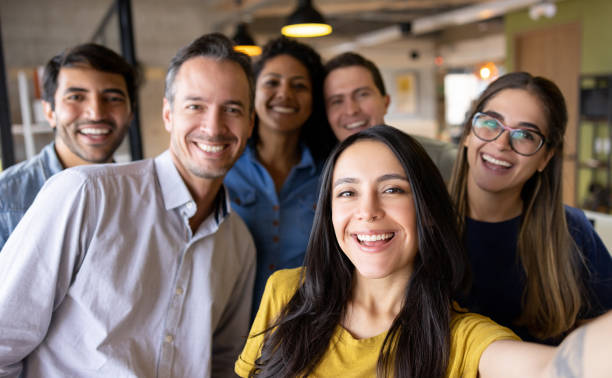
\includegraphics[width=0.9\textwidth]{foto-kelompok}\par
		
		% ---------- Disusun oleh ----------
		\vspace{1.2cm}
		{\bfseries Disusun oleh:\par}
		\vspace{0.5cm} 
		\begin{tabular}{l l}
			Agatha Tatianingseto & (13524008) \\
			Muhammad Nur Majiid & (13524028) \\
		\end{tabular}
		
		% ---------- Institusi ----------
		\vspace{2.0cm}
		Laboratorium Ilmu dan Rekayasa Komputasi\par
		Program Studi Teknik Informatika\par
		Sekolah Teknik Elektro dan Informatika\par
		Institut Teknologi Bandung\par
		
	\end{titlepage}
	
	\clearpage
	\pagestyle{fancy}
	
	\tableofcontents
	\clearpage
	
	\chapter{Algoritma Pathfinding}
	% ============================================================
% BAGIAN 1 - ALGORITMA PATHFINDING
% ============================================================

Permasalahan \textit{Ice Sliding Puzzle Solver} pada tugas ini diselesaikan sebagai persoalan pencarian jalur pada ruang state. 
Berbeda dengan pathfinding biasa yang umumnya bergerak satu petak setiap langkah, pada puzzle ini aktor bergerak secara \textit{sliding}, yaitu terus berjalan pada satu arah sampai tepat sebelum menabrak rintangan. 
Oleh karena itu, satu aksi gerakan dapat melewati beberapa tile sekaligus dan cost gerakannya dihitung dari seluruh tile yang dilalui.

\begin{tcolorbox}[
	colback=blue!5,
	colframe=blue!60!black,
	title=\textbf{Inti Permasalahan Pathfinding},
	arc=2mm,
	boxrule=0.8pt
]
Algoritma harus mencari urutan gerakan dari posisi awal \texttt{Z} menuju titik tujuan \texttt{O}, dengan syarat aktor harus melewati angka secara berurutan dari \texttt{0} sampai angka terbesar yang ada pada papan. 
Solusi hanya dianggap valid apabila aktor berhenti tepat di \texttt{O} dan seluruh angka yang diperlukan sudah dilewati sesuai urutan.
\end{tcolorbox}

\section{Representasi State}

Setiap konfigurasi pencarian direpresentasikan sebagai sebuah state. 
State tidak cukup hanya menyimpan posisi aktor, karena permainan juga memiliki constraint angka berurutan. 
Oleh karena itu, state juga menyimpan informasi angka yang sudah dikumpulkan, angka terakhir yang valid, path gerakan, serta cost yang sudah dikeluarkan.

\begin{table}[H]
	\centering
	\caption{Representasi state pada algoritma pathfinding}
	\begin{tabular}{|p{4cm}|p{10cm}|}
		\hline
		\rowcolor{blue!15}
		\textbf{Komponen State} & \textbf{Keterangan} \\
		\hline
		Posisi aktor & Menyimpan koordinat baris dan kolom aktor pada papan. \\
		\hline
		\textit{Collected mask} & Menyimpan himpunan angka yang sudah dikumpulkan dalam bentuk bitmask. \\
		\hline
		Angka terakhir & Menyimpan angka terakhir yang berhasil dilewati secara valid. Nilai awalnya adalah $-1$. \\
		\hline
		Path gerakan & Menyimpan urutan gerakan yang sudah dilakukan, misalnya \texttt{RULDR}. \\
		\hline
		Total cost & Menyimpan akumulasi cost dari seluruh gerakan sliding yang sudah dilakukan. \\
		\hline
		Nilai heuristik & Digunakan oleh GBFS dan A* untuk memperkirakan kedekatan state terhadap target berikutnya. \\
		\hline
	\end{tabular}
\end{table}

Secara umum, identitas sebuah state ditentukan oleh kombinasi posisi aktor dan progres angka yang sudah dikumpulkan. 
Dua state dengan posisi aktor sama belum tentu setara apabila angka yang sudah dikumpulkan berbeda. 
Sebagai contoh, aktor yang berada pada posisi yang sama tetapi sudah mengumpulkan angka \texttt{0} memiliki kondisi pencarian yang berbeda dengan aktor yang belum mengumpulkan angka tersebut.

\section{Mekanisme Ekspansi State}

Pada setiap state, algoritma mencoba empat arah gerakan, yaitu atas, bawah, kiri, dan kanan. 
Arah tersebut direpresentasikan dengan karakter \texttt{U}, \texttt{D}, \texttt{L}, dan \texttt{R}. 
Setiap gerakan diproses menggunakan mekanisme sliding sampai aktor berhenti, keluar papan, melewati lava, atau melanggar aturan angka.

\begin{table}[H]
	\centering
	\caption{Aturan ekspansi gerakan}
	\begin{tabular}{|p{3.5cm}|p{10.5cm}|}
		\hline
		\rowcolor{gray!20}
		\textbf{Kondisi} & \textbf{Penanganan} \\
		\hline
		Menabrak \texttt{X} & Aktor berhenti tepat sebelum rintangan. Tile \texttt{X} tidak dilewati dan cost-nya tidak dihitung. \\
		\hline
		Melewati \texttt{L} & Gerakan dianggap menyebabkan \textit{game over}, sehingga state hasil tidak diproses. \\
		\hline
		Keluar papan & Jika aktor bergerak keluar batas papan tanpa tertahan rintangan, gerakan dianggap tidak valid. \\
		\hline
		Melewati angka benar & Angka diterima jika nilainya sama dengan angka terakhir yang dikumpulkan ditambah satu. \\
		\hline
		Melewati angka salah & Gerakan dianggap tidak valid karena melanggar constraint urutan angka. \\
		\hline
		Berhenti di \texttt{O} & State menjadi goal hanya jika seluruh angka sudah dikumpulkan sesuai urutan. \\
		\hline
	\end{tabular}
\end{table}

\begin{tcolorbox}[
	colback=gray!5,
	colframe=black!60,
	title=\textbf{Skema Umum Ekspansi State},
	arc=2mm,
	boxrule=0.8pt
]
\begin{center}
\begin{forest}
for tree={
	draw,
	rounded corners,
	align=center,
	parent anchor=south,
	child anchor=north,
	l sep=8mm,
	s sep=8mm,
	font=\small
}
[State saat ini
	[Coba \texttt{U}]
	[Coba \texttt{D}]
	[Coba \texttt{L}]
	[Coba \texttt{R}]
]
\end{forest}
\end{center}

Setiap arah tidak langsung menghasilkan perpindahan satu petak, melainkan disimulasikan sebagai gerakan sliding sampai kondisi berhenti atau kondisi tidak valid ditemukan.
\end{tcolorbox}

\section{Uniform Cost Search}

Uniform Cost Search atau UCS adalah algoritma pencarian yang memilih state berdasarkan total cost aktual paling kecil. 
Pada permasalahan ini, UCS digunakan untuk mencari solusi dengan cost minimum, karena setiap tile memiliki nilai cost yang berbeda-beda. 
Dengan demikian, jalur yang memiliki jumlah gerakan lebih sedikit belum tentu merupakan jalur terbaik apabila melewati tile dengan cost besar.

\begin{tcolorbox}[
	colback=green!5,
	colframe=green!50!black,
	title=\textbf{Prinsip UCS},
	arc=2mm,
	boxrule=0.8pt
]
UCS selalu memilih state dengan nilai $g(n)$ terkecil.
\[
	g(n) = \text{total cost dari start sampai state } n
\]
Dengan strategi ini, UCS memprioritaskan jalur yang benar-benar paling murah berdasarkan cost yang sudah dikeluarkan.
\end{tcolorbox}

\subsection{Langkah Kerja UCS}

\begin{longtable}{|p{1.2cm}|p{12.8cm}|}
	\caption{Langkah kerja Uniform Cost Search} \\
	\hline
	\rowcolor{green!15}
	\textbf{No.} & \textbf{Langkah} \\
	\hline
	\endfirsthead
	
	\hline
	\rowcolor{green!15}
	\textbf{No.} & \textbf{Langkah} \\
	\hline
	\endhead
	
	1 & Membuat initial state dari posisi awal aktor dengan cost awal $0$, angka terakhir $-1$, dan path kosong. \\
	\hline
	2 & Memasukkan initial state ke dalam priority queue. \\
	\hline
	3 & Mengambil state dengan nilai $g(n)$ terkecil dari priority queue. \\
	\hline
	4 & Memeriksa apakah state tersebut sudah memenuhi kondisi goal. \\
	\hline
	5 & Jika belum goal, algoritma mengekspansi state ke empat arah: \texttt{U}, \texttt{D}, \texttt{L}, dan \texttt{R}. \\
	\hline
	6 & Untuk setiap arah, dilakukan simulasi sliding sampai aktor berhenti atau gerakan menjadi tidak valid. \\
	\hline
	7 & Jika gerakan valid, cost baru dihitung dengan menambahkan cost sliding ke cost state saat ini. \\
	\hline
	8 & State baru dimasukkan ke priority queue apabila belum pernah dicapai sebelumnya dengan cost yang lebih kecil atau sama. \\
	\hline
	9 & Proses diulang sampai solusi ditemukan atau priority queue kosong. \\
	\hline
\end{longtable}

\subsection{Struktur Data UCS}

\begin{table}[H]
	\centering
	\caption{Struktur data yang digunakan pada UCS}
	\begin{tabular}{|p{4cm}|p{10cm}|}
		\hline
		\rowcolor{green!15}
		\textbf{Struktur Data} & \textbf{Fungsi} \\
		\hline
		Priority queue & Menyimpan state yang akan diproses, dengan prioritas berdasarkan nilai $g(n)$ terkecil. \\
		\hline
		Map best cost & Menyimpan cost terbaik untuk setiap kombinasi posisi dan collected mask. \\
		\hline
		State & Menyimpan posisi aktor, path, cost, collected mask, dan angka terakhir. \\
		\hline
		MoveResult & Menyimpan hasil simulasi sliding, seperti posisi baru, cost gerakan, tile yang dilewati, dan status validitas gerakan. \\
		\hline
	\end{tabular}
\end{table}

\subsection{Kelebihan dan Kekurangan UCS}

\begin{table}[H]
	\centering
	\caption{Kelebihan dan kekurangan UCS}
	\begin{tabular}{|p{3cm}|p{11cm}|}
		\hline
		\rowcolor{green!15}
		\textbf{Aspek} & \textbf{Penjelasan} \\
		\hline
		Kelebihan & UCS dapat menghasilkan solusi optimal terhadap total cost selama semua cost bernilai positif. Hal ini cocok untuk puzzle yang memiliki variasi cost pada setiap tile. \\
		\hline
		Kekurangan & UCS dapat meninjau banyak konfigurasi karena tidak memiliki informasi estimasi arah menuju target. Pada papan besar atau konfigurasi kompleks, jumlah state yang dieksplorasi dapat menjadi sangat besar. \\
		\hline
	\end{tabular}
\end{table}

\section{Greedy Best-First Search}

Greedy Best-First Search atau GBFS adalah algoritma pathfinding yang memilih state berdasarkan nilai heuristik terkecil. 
Berbeda dengan UCS yang memperhatikan total cost aktual, GBFS lebih fokus pada state yang terlihat paling dekat dengan target berikutnya. 
Target berikutnya dapat berupa angka yang harus dikumpulkan selanjutnya atau titik tujuan \texttt{O} apabila seluruh angka sudah terkumpul.

\begin{tcolorbox}[
	colback=orange!5,
	colframe=orange!70!black,
	title=\textbf{Prinsip GBFS},
	arc=2mm,
	boxrule=0.8pt
]
GBFS selalu memilih state dengan nilai $h(n)$ terkecil.
\[
	h(n) = \text{estimasi jarak dari state } n \text{ menuju target berikutnya}
\]
Algoritma ini bersifat rakus karena hanya mempertimbangkan estimasi terdekat, bukan total cost aktual dari start.
\end{tcolorbox}

\subsection{Langkah Kerja GBFS}

\begin{longtable}{|p{1.2cm}|p{12.8cm}|}
	\caption{Langkah kerja Greedy Best-First Search} \\
	\hline
	\rowcolor{orange!20}
	\textbf{No.} & \textbf{Langkah} \\
	\hline
	\endfirsthead
	
	\hline
	\rowcolor{orange!20}
	\textbf{No.} & \textbf{Langkah} \\
	\hline
	\endhead
	
	1 & Membuat initial state dari posisi awal aktor. \\
	\hline
	2 & Menghitung nilai heuristik initial state terhadap target berikutnya. \\
	\hline
	3 & Memasukkan initial state ke priority queue dengan prioritas berdasarkan $h(n)$. \\
	\hline
	4 & Mengambil state dengan nilai heuristik terkecil. \\
	\hline
	5 & Memeriksa apakah state sudah memenuhi kondisi goal. \\
	\hline
	6 & Jika belum goal, state diekspansi ke empat arah gerakan. \\
	\hline
	7 & Untuk setiap arah, dilakukan simulasi sliding dengan tetap memperhatikan rintangan, lava, batas papan, dan urutan angka. \\
	\hline
	8 & Jika gerakan valid, state baru dihitung nilai heuristiknya. \\
	\hline
	9 & State baru dimasukkan ke priority queue apabila layak untuk diproses. \\
	\hline
	10 & Proses berlanjut sampai solusi ditemukan atau tidak ada state tersisa. \\
	\hline
\end{longtable}

\subsection{Heuristik pada GBFS}

Heuristik digunakan untuk memperkirakan kedekatan aktor terhadap target yang sedang dikejar. 
Jika masih ada angka yang belum dikumpulkan, maka target heuristik adalah angka berikutnya. 
Jika seluruh angka sudah dikumpulkan, maka target heuristik adalah titik tujuan \texttt{O}.

\begin{table}[H]
	\centering
	\caption{Peran heuristik pada GBFS}
	\begin{tabular}{|p{4cm}|p{10cm}|}
		\hline
		\rowcolor{orange!20}
		\textbf{Aspek} & \textbf{Penjelasan} \\
		\hline
		Target heuristik & Angka berikutnya yang harus dikumpulkan, atau \texttt{O} jika semua angka sudah terkumpul. \\
		\hline
		Dasar prioritas & State dengan nilai heuristik lebih kecil akan diproses lebih dahulu. \\
		\hline
		Hubungan dengan cost & Cost aktual tetap dihitung untuk total solusi, tetapi tidak menjadi prioritas utama dalam pemilihan state. \\
		\hline
		Hubungan dengan sliding & Heuristik hanya mengarahkan pencarian, sedangkan validitas gerakan tetap ditentukan oleh hasil simulasi sliding. \\
		\hline
	\end{tabular}
\end{table}

\begin{tcolorbox}[
	colback=orange!5,
	colframe=orange!70!black,
	title=\textbf{Ilustrasi Keputusan GBFS},
	arc=2mm,
	boxrule=0.8pt
]
\begin{center}
\begin{tabular}{c c c}
\textbf{State A} & \textbf{State B} & \textbf{State C} \\
$h(n)=8$ & $h(n)=3$ & $h(n)=5$ \\
\end{tabular}
\end{center}

GBFS akan memilih \textbf{State B} terlebih dahulu karena memiliki nilai heuristik paling kecil, meskipun cost aktual dari start menuju State B belum tentu paling kecil.
\end{tcolorbox}

\subsection{Kelebihan dan Kekurangan GBFS}

\begin{table}[H]
	\centering
	\caption{Kelebihan dan kekurangan GBFS}
	\begin{tabular}{|p{3cm}|p{11cm}|}
		\hline
		\rowcolor{orange!20}
		\textbf{Aspek} & \textbf{Penjelasan} \\
		\hline
		Kelebihan & GBFS cenderung lebih cepat menemukan solusi karena pencariannya diarahkan oleh heuristik menuju target berikutnya. \\
		\hline
		Kekurangan & GBFS tidak selalu menghasilkan solusi optimal karena tidak memprioritaskan total cost aktual. State yang tampak dekat ke target bisa saja melalui jalur dengan cost besar. \\
		\hline
	\end{tabular}
\end{table}

\section{A*}

A* adalah algoritma pathfinding yang menggabungkan prinsip UCS dan GBFS. 
Algoritma ini tidak hanya memperhatikan cost aktual dari start menuju state saat ini, tetapi juga memperhitungkan estimasi cost menuju target berikutnya. 
Dengan demikian, A* berusaha menyeimbangkan pencarian yang murah secara cost dan pencarian yang terarah menuju goal.

\begin{tcolorbox}[
	colback=red!5,
	colframe=red!60!black,
	title=\textbf{Prinsip A*},
	arc=2mm,
	boxrule=0.8pt
]
A* memilih state berdasarkan nilai $f(n)$ terkecil.
\[
	f(n) = g(n) + h(n)
\]
dengan:
\[
	g(n) = \text{cost aktual dari start ke state } n
\]
\[
	h(n) = \text{estimasi cost dari state } n \text{ ke target berikutnya}
\]
\end{tcolorbox}

\subsection{Langkah Kerja A*}

\begin{longtable}{|p{1.2cm}|p{12.8cm}|}
	\caption{Langkah kerja A*} \\
	\hline
	\rowcolor{red!15}
	\textbf{No.} & \textbf{Langkah} \\
	\hline
	\endfirsthead
	
	\hline
	\rowcolor{red!15}
	\textbf{No.} & \textbf{Langkah} \\
	\hline
	\endhead
	
	1 & Membuat initial state dengan $g(n)=0$ dan path kosong. \\
	\hline
	2 & Menghitung nilai heuristik $h(n)$ untuk initial state. \\
	\hline
	3 & Menghitung nilai $f(n)=g(n)+h(n)$ dan memasukkan state ke priority queue. \\
	\hline
	4 & Mengambil state dengan nilai $f(n)$ terkecil dari priority queue. \\
	\hline
	5 & Memeriksa apakah state sudah memenuhi kondisi goal. \\
	\hline
	6 & Jika belum goal, state diekspansi ke empat arah gerakan. \\
	\hline
	7 & Untuk setiap gerakan valid, algoritma menghitung cost sliding dan memperbarui nilai $g(n)$. \\
	\hline
	8 & Algoritma menghitung nilai $h(n)$ untuk state baru berdasarkan target berikutnya. \\
	\hline
	9 & Nilai $f(n)$ state baru dihitung dari $g(n)+h(n)$. \\
	\hline
	10 & State baru diproses hanya jika cost-nya lebih baik daripada kunjungan sebelumnya pada posisi dan collected mask yang sama. \\
	\hline
	11 & Proses diulang sampai solusi ditemukan atau seluruh kemungkinan state habis. \\
	\hline
\end{longtable}

\subsection{Peran $g(n)$, $h(n)$, dan $f(n)$}

\begin{table}[H]
	\centering
	\caption{Definisi fungsi biaya pada A*}
	\begin{tabular}{|p{3cm}|p{11cm}|}
		\hline
		\rowcolor{red!15}
		\textbf{Fungsi} & \textbf{Makna} \\
		\hline
		$g(n)$ & Total cost aktual dari initial state menuju state $n$. Nilainya bertambah berdasarkan cost seluruh tile yang dilewati selama sliding. \\
		\hline
		$h(n)$ & Estimasi cost dari state $n$ menuju target berikutnya. Target dapat berupa angka berikutnya atau titik tujuan \texttt{O}. \\
		\hline
		$f(n)$ & Nilai prioritas state pada A*, yaitu gabungan antara cost aktual dan estimasi menuju target. \\
		\hline
	\end{tabular}
\end{table}

\subsection{Struktur Data A*}

\begin{table}[H]
	\centering
	\caption{Struktur data yang digunakan pada A*}
	\begin{tabular}{|p{4cm}|p{10cm}|}
		\hline
		\rowcolor{red!15}
		\textbf{Struktur Data} & \textbf{Fungsi} \\
		\hline
		Priority queue & Menyimpan state yang akan diproses dengan prioritas berdasarkan nilai $f(n)$ terkecil. \\
		\hline
		Map best cost & Menyimpan cost terbaik untuk setiap kombinasi posisi aktor dan collected mask. \\
		\hline
		State & Menyimpan posisi, path, $g(n)$, $h(n)$, collected mask, dan angka terakhir. \\
		\hline
		Heuristic & Menghitung estimasi jarak atau cost menuju target berikutnya. \\
		\hline
		Movement engine & Mensimulasikan gerakan sliding dan menentukan validitas hasil gerakan. \\
		\hline
	\end{tabular}
\end{table}

\subsection{Kelebihan dan Kekurangan A*}

\begin{table}[H]
	\centering
	\caption{Kelebihan dan kekurangan A*}
	\begin{tabular}{|p{3cm}|p{11cm}|}
		\hline
		\rowcolor{red!15}
		\textbf{Aspek} & \textbf{Penjelasan} \\
		\hline
		Kelebihan & A* lebih terarah dibanding UCS karena menggunakan heuristik, tetapi tetap mempertimbangkan cost aktual. Jika heuristik yang digunakan admissible, A* dapat menghasilkan solusi optimal. \\
		\hline
		Kekurangan & Performa A* sangat bergantung pada kualitas heuristik. Jika heuristik kurang informatif, A* dapat berperilaku mirip UCS dan tetap mengeksplorasi banyak state. \\
		\hline
	\end{tabular}
\end{table}

\section{Perbandingan UCS, GBFS, dan A*}

Ketiga algoritma memiliki strategi pemilihan state yang berbeda. 
UCS berfokus pada cost aktual, GBFS berfokus pada estimasi ke target, sedangkan A* menggabungkan keduanya. 
Perbandingan ini penting karena karakteristik puzzle dipengaruhi oleh dua hal utama, yaitu cost tile yang bervariasi dan posisi target yang harus dicapai secara berurutan.

\begin{table}[H]
	\centering
	\caption{Perbandingan algoritma pathfinding}
	\begin{tabular}{|p{3cm}|p{3.5cm}|p{3.5cm}|p{3.5cm}|}
		\hline
		\rowcolor{gray!25}
		\textbf{Aspek} & \textbf{UCS} & \textbf{GBFS} & \textbf{A*} \\
		\hline
		Dasar prioritas & $g(n)$ & $h(n)$ & $f(n)=g(n)+h(n)$ \\
		\hline
		Memperhatikan cost aktual & Ya & Tidak sebagai prioritas utama & Ya \\
		\hline
		Menggunakan heuristik & Tidak & Ya & Ya \\
		\hline
		Kecepatan pencarian & Cenderung lebih lambat & Cenderung lebih cepat & Bergantung kualitas heuristik \\
		\hline
		Optimalitas solusi & Optimal untuk cost positif & Tidak selalu optimal & Optimal jika heuristik admissible \\
		\hline
		Kelemahan utama & Eksplorasi state besar & Dapat memilih jalur mahal & Bergantung pada heuristik \\
		\hline
	\end{tabular}
\end{table}

\begin{tcolorbox}[
	colback=purple!5,
	colframe=purple!60!black,
	title=\textbf{Ringkasan Pemilihan Algoritma},
	arc=2mm,
	boxrule=0.8pt
]
\begin{itemize}
	\item UCS cocok digunakan ketika prioritas utama adalah mendapatkan solusi dengan total cost minimum.
	\item GBFS cocok digunakan ketika pencarian ingin diarahkan secepat mungkin menuju target, meskipun tidak menjamin solusi optimal.
	\item A* menjadi pendekatan yang lebih seimbang karena mempertimbangkan cost aktual dan estimasi menuju target.
\end{itemize}
\end{tcolorbox}
	
	\chapter{Analisa Algoritma Pathfinding}
	% ============================================================
% BAGIAN 2 - ANALISIS ALGORITMA PATHFINDING
% ============================================================

Bagian ini membahas analisis terhadap algoritma UCS, GBFS, dan A* yang digunakan pada penyelesaian \textit{Ice Sliding Puzzle Solver}. 
Analisis dilakukan dari sisi fungsi evaluasi, heuristik, optimalitas, kompleksitas, ruang state, serta kesesuaian algoritma terhadap karakteristik khusus puzzle.

\section{Definisi Cost dan Fungsi Evaluasi}

Pada permasalahan ini, cost tidak dihitung berdasarkan jumlah aksi saja, melainkan berdasarkan total cost tile yang dilewati selama aktor melakukan gerakan sliding. 
Tile awal sebelum gerakan tidak dihitung, sedangkan tile tempat aktor berhenti tetap dihitung karena tile tersebut termasuk tile yang dilewati.

\begin{tcolorbox}[
	colback=blue!5,
	colframe=blue!60!black,
	title=\textbf{Definisi Cost Gerakan},
	arc=2mm,
	boxrule=0.8pt
]
Jika dalam satu gerakan sliding aktor melewati tile dengan cost $c_1, c_2, \ldots, c_k$, maka cost gerakan tersebut adalah:
\[
	C_{\text{move}} = \sum_{i=1}^{k} c_i
\]
Total cost solusi adalah penjumlahan cost seluruh gerakan sliding:
\[
	C_{\text{total}} = \sum_{j=1}^{m} C_{\text{move}_j}
\]
dengan $m$ menyatakan banyaknya aksi gerakan dalam solusi.
\end{tcolorbox}

\begin{table}[H]
	\centering
	\caption{Definisi $g(n)$, $h(n)$, dan $f(n)$ pada setiap algoritma}
	\begin{tabular}{|p{2.7cm}|p{3.7cm}|p{3.7cm}|p{3.7cm}|}
		\hline
		\rowcolor{gray!25}
		\textbf{Algoritma} & \textbf{$g(n)$} & \textbf{$h(n)$} & \textbf{$f(n)$ / Prioritas} \\
		\hline
		UCS & Total cost aktual dari start ke state $n$. & Tidak digunakan. & $f(n)=g(n)$ \\
		\hline
		GBFS & Tetap dapat disimpan sebagai total cost solusi, tetapi tidak menjadi dasar prioritas. & Estimasi jarak atau cost dari state $n$ ke target berikutnya. & $f(n)=h(n)$ \\
		\hline
		A* & Total cost aktual dari start ke state $n$. & Estimasi jarak atau cost dari state $n$ ke target berikutnya. & $f(n)=g(n)+h(n)$ \\
		\hline
	\end{tabular}
\end{table}

\begin{tcolorbox}[
	colback=gray!5,
	colframe=black!60,
	title=\textbf{Perbedaan Utama Fungsi Evaluasi},
	arc=2mm,
	boxrule=0.8pt
]
\begin{itemize}
	\item UCS bersifat \textit{cost-based} karena hanya memilih state berdasarkan cost aktual terkecil.
	\item GBFS bersifat \textit{heuristic-based} karena hanya memilih state berdasarkan estimasi kedekatan ke target.
	\item A* bersifat gabungan karena mempertimbangkan cost aktual dan estimasi menuju target.
\end{itemize}
\end{tcolorbox}

\begin{table}[H]
	\centering
	\caption{Contoh konseptual pemilihan state berdasarkan fungsi evaluasi}
	\begin{tabular}{|p{2.3cm}|p{2.5cm}|p{2.5cm}|p{2.5cm}|p{3cm}|}
		\hline
		\rowcolor{blue!15}
		\textbf{State} & \textbf{$g(n)$} & \textbf{$h(n)$} & \textbf{$g(n)+h(n)$} & \textbf{Dipilih oleh} \\
		\hline
		A & 10 & 8 & 18 & UCS \\
		\hline
		B & 14 & 3 & 17 & GBFS dan A* \\
		\hline
		C & 12 & 6 & 18 & Tidak dipilih lebih awal \\
		\hline
	\end{tabular}
\end{table}

Pada contoh di atas, UCS memilih state A karena memiliki $g(n)$ terkecil. 
GBFS memilih state B karena memiliki $h(n)$ terkecil. 
A* juga memilih state B karena memiliki nilai $g(n)+h(n)$ terkecil.

\section{Analisis Heuristik}

Heuristik digunakan pada GBFS dan A* untuk memperkirakan kedekatan suatu state terhadap target berikutnya. 
Target berikutnya tidak selalu berupa titik tujuan \texttt{O}. 
Jika masih terdapat angka yang belum dikumpulkan, maka target berikutnya adalah angka yang harus dilewati sesuai urutan. 
Setelah seluruh angka terkumpul, barulah target heuristik diarahkan ke titik tujuan.

\begin{tcolorbox}[
	colback=orange!5,
	colframe=orange!70!black,
	title=\textbf{Target Heuristik},
	arc=2mm,
	boxrule=0.8pt
]
\[
	\text{Target}(n) =
	\begin{cases}
		\text{posisi angka berikutnya}, & \text{jika masih ada angka yang belum dikumpulkan} \\
		\text{posisi goal } O, & \text{jika semua angka sudah dikumpulkan}
	\end{cases}
\]
\end{tcolorbox}

\subsection{Heuristik Utama}

Heuristik utama yang umum digunakan pada grid adalah jarak Manhattan. 
Jarak Manhattan menghitung selisih absolut baris dan kolom antara posisi aktor dengan target.

\begin{tcolorbox}[
	colback=orange!5,
	colframe=orange!70!black,
	title=\textbf{Heuristik Manhattan Distance},
	arc=2mm,
	boxrule=0.8pt
]
Misalkan posisi aktor adalah $(r_1,c_1)$ dan posisi target adalah $(r_2,c_2)$, maka:
\[
	h(n)=|r_1-r_2|+|c_1-c_2|
\]
Heuristik ini dipilih karena sederhana, cepat dihitung, dan sesuai dengan papan berbentuk grid yang gerakannya hanya horizontal atau vertikal.
\end{tcolorbox}

\subsection{Heuristik Alternatif}

Apabila mengerjakan bonus heuristik, beberapa alternatif heuristik dapat digunakan untuk membandingkan performa pencarian. 
Setiap heuristik memiliki karakteristik yang berbeda terhadap akurasi estimasi dan waktu komputasi.

\begin{longtable}{|p{3.5cm}|p{5cm}|p{5.5cm}|}
	\caption{Contoh heuristik utama dan alternatif} \\
	\hline
	\rowcolor{orange!20}
	\textbf{Heuristik} & \textbf{Rumus / Ide} & \textbf{Karakteristik} \\
	\hline
	\endfirsthead
	
	\hline
	\rowcolor{orange!20}
	\textbf{Heuristik} & \textbf{Rumus / Ide} & \textbf{Karakteristik} \\
	\hline
	\endhead
	
	Manhattan Distance & $|r_1-r_2|+|c_1-c_2|$ & Cepat dihitung dan cocok untuk grid 4 arah, tetapi belum memperhitungkan sliding, obstacle, lava, dan cost tile. \\
	\hline
	Euclidean Distance & $\sqrt{(r_1-r_2)^2+(c_1-c_2)^2}$ & Mengukur jarak garis lurus, tetapi kurang merepresentasikan gerakan grid yang hanya horizontal dan vertikal. \\
	\hline
	Minimum Tile Cost Weighted Manhattan & Manhattan Distance dikalikan cost tile minimum yang dapat dilewati. & Lebih dekat ke estimasi cost karena mempertimbangkan batas bawah cost tile, tetapi tetap belum sepenuhnya memperhitungkan sliding dan obstacle. \\
	\hline
	Remaining Target Estimate & Estimasi dari posisi saat ini ke angka berikutnya, lalu dilanjutkan secara kasar ke target-target berikutnya. & Dapat lebih informatif, tetapi perlu hati-hati agar tidak melebih-lebihkan estimasi jika digunakan pada A*. \\
	\hline
\end{longtable}

\subsection{Aspek yang Dipertimbangkan Heuristik}

Tidak semua heuristik memperhitungkan seluruh aturan pada Ice Sliding Puzzle. 
Beberapa heuristik hanya memperkirakan jarak geometris, sedangkan validitas gerakan tetap ditentukan oleh simulasi sliding.

\begin{table}[H]
	\centering
	\caption{Aspek puzzle yang dipertimbangkan oleh heuristik}
	\begin{tabular}{|p{5cm}|p{2.5cm}|p{6cm}|}
		\hline
		\rowcolor{orange!20}
		\textbf{Aspek} & \textbf{Dipertimbangkan?} & \textbf{Keterangan} \\
		\hline
		Posisi goal & Ya & Goal digunakan sebagai target apabila seluruh angka sudah terkumpul. \\
		\hline
		Posisi angka berikutnya & Ya & Jika masih ada angka, heuristik diarahkan ke angka berikutnya. \\
		\hline
		Sliding movement & Tidak langsung & Heuristik jarak hanya memberi estimasi; gerakan sliding tetap divalidasi oleh mekanisme ekspansi. \\
		\hline
		Cost tile & Tergantung heuristik & Manhattan biasa tidak memperhitungkan cost tile, sedangkan weighted heuristic dapat memasukkan cost minimum. \\
		\hline
		Obstacle & Tidak langsung & Obstacle tidak dihitung dalam rumus jarak sederhana, tetapi memengaruhi hasil validasi gerakan. \\
		\hline
		Lava & Tidak langsung & Lava tidak dihitung dalam heuristik sederhana, tetapi state yang melewati lava akan dibuang saat ekspansi. \\
		\hline
	\end{tabular}
\end{table}

\subsection{Admissibility Heuristik A*}

Heuristik dikatakan \textit{admissible} apabila tidak pernah melebih-lebihkan cost minimum sebenarnya dari suatu state menuju goal. 
Dengan kata lain, untuk setiap state $n$ berlaku:

\[
	h(n) \leq h^*(n)
\]

dengan $h^*(n)$ adalah cost optimal sebenarnya dari state $n$ menuju target.

\begin{tcolorbox}[
	colback=green!5,
	colframe=green!50!black,
	title=\textbf{Analisis Admissibility},
	arc=2mm,
	boxrule=0.8pt
]
Jika heuristik yang digunakan adalah Manhattan Distance murni, maka heuristik tersebut aman sebagai estimasi jarak geometris, tetapi belum tentu selalu menjadi estimasi cost yang ketat pada puzzle sliding. 
Apabila semua cost tile minimal bernilai $1$, Manhattan Distance dapat dipandang sebagai batas bawah sederhana terhadap jumlah perpindahan grid. 
Namun, karena satu aksi sliding dapat melewati banyak tile sekaligus dan struktur obstacle dapat membuat aktor harus mengambil rute tidak langsung, admissibility perlu dianalisis berdasarkan definisi cost yang digunakan.
\end{tcolorbox}

Untuk menjaga heuristik A* tetap admissible terhadap cost, heuristik yang lebih aman adalah menggunakan estimasi berbasis batas bawah cost tile, misalnya:

\[
	h(n)=d_{\text{Manhattan}}(n,\text{target}) \times c_{\min}
\]

dengan $c_{\min}$ adalah cost minimum dari tile yang dapat dilewati. 
Jika $c_{\min}$ tidak melebihi cost traversal mana pun, maka estimasi ini tidak akan melebihi cost aktual minimum secara langsung terhadap jarak grid. 
Namun, tetap perlu dicatat bahwa karakter sliding dapat membuat estimasi ini tidak selalu sangat informatif.

\subsection{Konsistensi Heuristik}

Heuristik dikatakan konsisten atau monotonic apabila untuk setiap state $n$ dan successor $n'$ berlaku:

\[
	h(n) \leq c(n,n') + h(n')
\]

dengan $c(n,n')$ adalah cost gerakan dari $n$ ke $n'$.

\begin{table}[H]
	\centering
	\caption{Hubungan heuristik dengan performa pencarian}
	\begin{tabular}{|p{4cm}|p{10cm}|}
		\hline
		\rowcolor{orange!20}
		\textbf{Kualitas Heuristik} & \textbf{Dampak terhadap Algoritma} \\
		\hline
		Terlalu kecil & A* menjadi mirip UCS karena estimasi kurang membantu mengarahkan pencarian. \\
		\hline
		Terlalu besar & A* berisiko kehilangan jaminan optimalitas jika heuristik tidak admissible. \\
		\hline
		Informatif dan admissible & A* dapat mengurangi jumlah iterasi tanpa mengorbankan optimalitas. \\
		\hline
		Tidak mempertimbangkan obstacle/lava & Algoritma dapat mengejar target yang tampak dekat, tetapi sebenarnya sulit atau tidak valid dicapai. \\
		\hline
	\end{tabular}
\end{table}

\section{Analisis Optimalitas}

Optimalitas menunjukkan apakah algoritma dapat menjamin solusi dengan total cost paling minimum. 
Pada Ice Sliding Puzzle, optimalitas sangat bergantung pada cara algoritma memilih state dan bagaimana cost tile diperhitungkan.

\begin{table}[H]
	\centering
	\caption{Analisis optimalitas algoritma}
	\begin{tabular}{|p{3cm}|p{3cm}|p{8cm}|}
		\hline
		\rowcolor{green!15}
		\textbf{Algoritma} & \textbf{Optimal?} & \textbf{Alasan} \\
		\hline
		UCS & Ya & UCS selalu memilih state dengan total cost aktual terkecil. Dengan cost tile positif, solusi pertama yang mencapai goal merupakan solusi dengan cost minimum. \\
		\hline
		GBFS & Tidak selalu & GBFS hanya memilih state berdasarkan heuristik terkecil. Jalur yang terlihat dekat ke target belum tentu memiliki total cost paling kecil. \\
		\hline
		A* & Ya, dengan syarat & A* optimal apabila heuristik yang digunakan admissible dan cost gerakan tidak negatif. Jika heuristik melebih-lebihkan cost, jaminan optimalitas dapat hilang. \\
		\hline
	\end{tabular}
\end{table}

\begin{tcolorbox}[
	colback=green!5,
	colframe=green!50!black,
	title=\textbf{Hubungan Admissibility dan Optimalitas A*},
	arc=2mm,
	boxrule=0.8pt
]
A* dapat menjamin solusi optimal jika heuristik tidak pernah melebih-lebihkan cost sebenarnya menuju goal. 
Jika $h(n)$ admissible, maka nilai $f(n)=g(n)+h(n)$ tidak akan membuat algoritma mengabaikan jalur yang sebenarnya lebih murah.
\end{tcolorbox}

Pengaruh cost tile juga penting dalam optimalitas. 
Pada papan dengan cost berbeda-beda, jalur yang secara visual lebih pendek dapat memiliki total cost lebih besar dibanding jalur yang lebih panjang tetapi melewati tile murah. 
Karena itu, algoritma yang memperhatikan $g(n)$, seperti UCS dan A*, lebih aman digunakan untuk mencari cost minimum dibanding GBFS.

\section{Analisis Kompleksitas}

Kompleksitas algoritma dipengaruhi oleh banyaknya state yang mungkin dibentuk, jumlah arah gerakan, serta struktur papan. 
Misalkan papan berukuran $N \times M$, jumlah posisi maksimum adalah $N \cdot M$. 
Jika terdapat $K$ angka wajib, maka progres angka dapat direpresentasikan dengan bitmask hingga $2^K$ kemungkinan. 
Namun, karena angka harus dikumpulkan secara berurutan, jumlah progres valid dalam praktik lebih kecil dibanding semua kombinasi bitmask.

\begin{tcolorbox}[
	colback=purple!5,
	colframe=purple!60!black,
	title=\textbf{Perkiraan Jumlah State},
	arc=2mm,
	boxrule=0.8pt
]
Secara umum, batas atas jumlah state dapat ditulis sebagai:
\[
	|S| = O(N \cdot M \cdot 2^K)
\]
dengan:
\begin{itemize}
	\item $N \cdot M$ adalah jumlah maksimum posisi pada papan,
	\item $K$ adalah jumlah angka wajib yang harus dikumpulkan,
	\item $2^K$ adalah kemungkinan kombinasi angka yang sudah dikumpulkan.
\end{itemize}
Karena angka harus dikumpulkan berurutan, jumlah state valid biasanya lebih kecil daripada batas atas tersebut.
\end{tcolorbox}

Pada setiap state, algoritma mencoba empat arah gerakan. 
Namun, satu gerakan sliding dapat memindai beberapa tile sampai berhenti. 
Dalam kasus terburuk, satu sliding dapat memeriksa hingga $O(\max(N,M))$ tile.

\[
	T_{\text{expand}} = O(4 \cdot \max(N,M))
\]

\begin{longtable}{|p{3cm}|p{5.2cm}|p{5.7cm}|}
	\caption{Kompleksitas waktu dan ruang algoritma} \\
	\hline
	\rowcolor{purple!15}
	\textbf{Algoritma} & \textbf{Kompleksitas Waktu} & \textbf{Kompleksitas Ruang} \\
	\hline
	\endfirsthead
	
	\hline
	\rowcolor{purple!15}
	\textbf{Algoritma} & \textbf{Kompleksitas Waktu} & \textbf{Kompleksitas Ruang} \\
	\hline
	\endhead
	
	UCS & $O(|S| \log |S| \cdot 4 \cdot \max(N,M))$ & $O(|S|)$ untuk priority queue dan best cost map. \\
	\hline
	GBFS & $O(|S| \log |S| \cdot 4 \cdot \max(N,M))$ pada kasus terburuk, tetapi sering lebih cepat jika heuristik efektif. & $O(|S|)$ untuk priority queue dan struktur visited/best cost. \\
	\hline
	A* & $O(|S| \log |S| \cdot 4 \cdot \max(N,M))$ pada kasus terburuk, tetapi dapat lebih efisien dari UCS jika heuristik informatif. & $O(|S|)$ untuk priority queue dan best cost map. \\
	\hline
\end{longtable}

\begin{table}[H]
	\centering
	\caption{Faktor yang memengaruhi kompleksitas}
	\begin{tabular}{|p{4.5cm}|p{9.5cm}|}
		\hline
		\rowcolor{purple!15}
		\textbf{Faktor} & \textbf{Pengaruh} \\
		\hline
		Ukuran papan $N \times M$ & Semakin besar papan, semakin banyak posisi yang mungkin menjadi state. \\
		\hline
		Jumlah angka wajib $K$ & Semakin banyak angka, semakin banyak variasi progres angka yang perlu disimpan. \\
		\hline
		Jumlah arah gerakan & Setiap state maksimal diekspansi ke 4 arah. \\
		\hline
		Panjang sliding & Semakin panjang lintasan sliding, semakin besar biaya simulasi satu aksi. \\
		\hline
		Obstacle & Dapat mengurangi area yang dapat dicapai, tetapi juga dapat membuat rute menjadi lebih kompleks. \\
		\hline
		Lava & Mengurangi jalur valid karena state yang melewati lava langsung dibuang. \\
		\hline
		Kualitas heuristik & Sangat memengaruhi GBFS dan A*, terutama dalam mengurangi jumlah iterasi. \\
		\hline
	\end{tabular}
\end{table}

\section{Analisis State Space}

State space adalah himpunan seluruh konfigurasi yang mungkin diproses oleh algoritma. 
Pada puzzle ini, state tidak cukup hanya menyimpan posisi aktor, karena aktor yang berada di posisi sama dapat memiliki kondisi berbeda tergantung angka yang sudah dikumpulkan.

\begin{tcolorbox}[
	colback=blue!5,
	colframe=blue!60!black,
	title=\textbf{Definisi State Space},
	arc=2mm,
	boxrule=0.8pt
]
Sebuah state dapat ditulis sebagai:
\[
	s = (pos, mask, last, path, g, h)
\]
dengan $pos$ adalah posisi aktor, $mask$ adalah penanda angka yang sudah dikumpulkan, $last$ adalah angka terakhir yang valid, $path$ adalah urutan gerakan, $g$ adalah total cost aktual, dan $h$ adalah nilai heuristik.
\end{tcolorbox}

\begin{table}[H]
	\centering
	\caption{Analisis komponen state space}
	\begin{tabular}{|p{4cm}|p{10cm}|}
		\hline
		\rowcolor{blue!15}
		\textbf{Komponen} & \textbf{Analisis} \\
		\hline
		Jumlah posisi maksimum & Sebanyak $N \cdot M$, tetapi posisi berupa obstacle tidak dapat ditempati. \\
		\hline
		Constraint angka & Membuat state harus membedakan progres angka yang sudah dikumpulkan. \\
		\hline
		Collected mask & Digunakan untuk menandai angka yang sudah dilewati tanpa perlu menyimpan list angka secara eksplisit. \\
		\hline
		State yang sama & Dua state dianggap sama jika posisi aktor dan collected mask sama. \\
		\hline
		State berbeda & Dua state dengan posisi sama tetapi collected mask berbeda tetap dianggap berbeda. \\
		\hline
		Pruning & State diabaikan jika sudah pernah dicapai dengan cost yang lebih kecil atau sama. \\
		\hline
	\end{tabular}
\end{table}

\begin{tcolorbox}[
	colback=gray!5,
	colframe=black!60,
	title=\textbf{Mengapa Posisi Saja Tidak Cukup?},
	arc=2mm,
	boxrule=0.8pt
]
Misalkan aktor berada pada posisi $(r,c)$. 
Jika pada kondisi pertama aktor sudah mengumpulkan angka \texttt{0}, sedangkan pada kondisi kedua belum, maka kedua kondisi tersebut tidak boleh dianggap sama. 
Hal ini karena langkah valid berikutnya berbeda: state pertama dapat mencari angka \texttt{1}, sedangkan state kedua masih harus mencari angka \texttt{0}.
\end{tcolorbox}

\section{Perbandingan Teoritis Algoritma}

Secara teoritis, UCS, GBFS, dan A* memiliki keunggulan pada aspek yang berbeda. 
UCS unggul dalam jaminan optimalitas, GBFS unggul dalam kecepatan pencarian jika heuristik baik, sedangkan A* mencoba menyeimbangkan keduanya.

\subsection{UCS vs GBFS}

\begin{table}[H]
	\centering
	\caption{Perbandingan UCS dan GBFS}
	\begin{tabular}{|p{4cm}|p{5cm}|p{5cm}|}
		\hline
		\rowcolor{gray!25}
		\textbf{Aspek} & \textbf{UCS} & \textbf{GBFS} \\
		\hline
		Dasar pemilihan state & Cost aktual $g(n)$ & Heuristik $h(n)$ \\
		\hline
		Optimalitas & Menjamin solusi cost minimum & Tidak menjamin solusi cost minimum \\
		\hline
		Jumlah iterasi & Cenderung lebih banyak & Cenderung lebih sedikit jika heuristik baik \\
		\hline
		Ketergantungan heuristik & Tidak bergantung heuristik & Sangat bergantung heuristik \\
		\hline
		Kesesuaian untuk cost berbeda & Sangat sesuai & Kurang aman untuk cost minimum \\
		\hline
	\end{tabular}
\end{table}

\subsection{UCS vs A*}

\begin{table}[H]
	\centering
	\caption{Perbandingan UCS dan A*}
	\begin{tabular}{|p{4cm}|p{5cm}|p{5cm}|}
		\hline
		\rowcolor{gray!25}
		\textbf{Aspek} & \textbf{UCS} & \textbf{A*} \\
		\hline
		Dasar pemilihan state & $g(n)$ & $g(n)+h(n)$ \\
		\hline
		Optimalitas & Optimal untuk cost positif & Optimal jika heuristik admissible \\
		\hline
		Arah pencarian & Tidak terarah ke goal & Lebih terarah ke target \\
		\hline
		Jumlah iterasi & Dapat sangat besar & Umumnya lebih sedikit jika heuristik informatif \\
		\hline
		Kelemahan & Tidak menggunakan estimasi & Bergantung kualitas heuristik \\
		\hline
	\end{tabular}
\end{table}

\subsection{GBFS vs A*}

\begin{table}[H]
	\centering
	\caption{Perbandingan GBFS dan A*}
	\begin{tabular}{|p{4cm}|p{5cm}|p{5cm}|}
		\hline
		\rowcolor{gray!25}
		\textbf{Aspek} & \textbf{GBFS} & \textbf{A*} \\
		\hline
		Dasar pemilihan state & $h(n)$ & $g(n)+h(n)$ \\
		\hline
		Kecepatan & Bisa sangat cepat & Biasanya lebih stabil \\
		\hline
		Optimalitas & Tidak dijamin & Dijamin jika heuristik admissible \\
		\hline
		Pengaruh cost aktual & Tidak menjadi prioritas utama & Selalu dipertimbangkan \\
		\hline
		Risiko & Terjebak pada jalur yang tampak dekat tetapi mahal & Lebih kecil karena mempertimbangkan cost aktual \\
		\hline
	\end{tabular}
\end{table}

\begin{longtable}{|p{4cm}|p{3.2cm}|p{3.2cm}|p{3.2cm}|}
	\caption{Ringkasan perbandingan teoritis UCS, GBFS, dan A*} \\
	\hline
	\rowcolor{gray!25}
	\textbf{Aspek} & \textbf{UCS} & \textbf{GBFS} & \textbf{A*} \\
	\hline
	\endfirsthead
	
	\hline
	\rowcolor{gray!25}
	\textbf{Aspek} & \textbf{UCS} & \textbf{GBFS} & \textbf{A*} \\
	\hline
	\endhead
	
	Optimalitas & Tinggi & Rendah & Tinggi jika heuristik admissible \\
	\hline
	Jumlah iterasi & Besar & Kecil jika heuristik baik & Sedang hingga kecil \\
	\hline
	Waktu eksekusi & Cenderung lebih lama & Cenderung lebih cepat & Bergantung heuristik \\
	\hline
	Penggunaan memori & Besar & Besar pada kasus buruk & Besar pada kasus buruk \\
	\hline
	Ketergantungan heuristik & Tidak ada & Sangat tinggi & Tinggi \\
	\hline
	Cocok untuk cost berbeda & Sangat cocok & Kurang cocok untuk cost minimum & Cocok jika heuristik baik \\
	\hline
\end{longtable}

\begin{tcolorbox}[
	colback=green!5,
	colframe=green!50!black,
	title=\textbf{Kesimpulan Teoritis},
	arc=2mm,
	boxrule=0.8pt
]
\begin{itemize}
	\item Algoritma yang paling aman untuk mencari cost minimum adalah UCS.
	\item Algoritma yang secara teoritis paling cepat menemukan solusi adalah GBFS, tetapi tidak menjamin cost minimum.
	\item Algoritma yang paling seimbang untuk Ice Sliding Puzzle adalah A*, karena menggabungkan cost aktual dan heuristik.
\end{itemize}
\end{tcolorbox}

\section{Analisis Khusus Ice Sliding Puzzle}

Ice Sliding Puzzle memiliki karakteristik yang berbeda dari pathfinding biasa. 
Pada pathfinding biasa, satu aksi umumnya berarti berpindah ke satu tile tetangga. 
Pada puzzle ini, satu aksi dapat melewati banyak tile karena aktor terus bergerak sampai berhenti di depan rintangan.

\begin{table}[H]
	\centering
	\caption{Perbedaan pathfinding biasa dan Ice Sliding Puzzle}
	\begin{tabular}{|p{4.5cm}|p{4.5cm}|p{5cm}|}
		\hline
		\rowcolor{cyan!15}
		\textbf{Aspek} & \textbf{Pathfinding Biasa} & \textbf{Ice Sliding Puzzle} \\
		\hline
		Satu aksi & Berpindah satu tile & Sliding hingga berhenti \\
		\hline
		Cost gerakan & Biasanya cost tile tujuan atau cost edge & Jumlah cost seluruh tile yang dilewati \\
		\hline
		Obstacle & Menghalangi perpindahan & Menjadi titik penghenti sliding \\
		\hline
		Lava & Tergantung aturan kasus & Selalu membuat path tidak valid jika dilewati \\
		\hline
		Keluar papan & Biasanya tidak diperbolehkan & Menyebabkan game over \\
		\hline
		Goal & Biasanya cukup mencapai posisi goal & Harus berhenti tepat di \texttt{O} \\
		\hline
		Constraint tambahan & Umumnya tidak ada & Angka harus dilewati berurutan \\
		\hline
	\end{tabular}
\end{table}

\begin{tcolorbox}[
	colback=cyan!5,
	colframe=cyan!60!black,
	title=\textbf{Dampak Karakteristik Sliding terhadap Algoritma},
	arc=2mm,
	boxrule=0.8pt
]
Karena satu aksi dapat melewati banyak tile, algoritma tidak dapat langsung memperlakukan tetangga state sebagai empat tile di sekitar aktor. 
Setiap ekspansi harus melakukan simulasi gerakan sampai aktor berhenti atau gerakan menjadi tidak valid. 
Hal ini membuat proses ekspansi lebih mahal dibanding pathfinding grid biasa.
\end{tcolorbox}

\begin{table}[H]
	\centering
	\caption{Aturan khusus puzzle dan dampaknya terhadap pencarian}
	\begin{tabular}{|p{4cm}|p{10cm}|}
		\hline
		\rowcolor{cyan!15}
		\textbf{Aturan} & \textbf{Dampak terhadap Algoritma} \\
		\hline
		Satu aksi adalah sliding & Successor state hanya terbentuk pada posisi akhir sliding, bukan pada setiap tile yang dilewati. \\
		\hline
		Cost seluruh tile dilewati & Algoritma harus menjumlahkan cost sepanjang lintasan sliding. \\
		\hline
		Lava menyebabkan game over & State hasil gerakan yang melewati lava harus langsung dibuang. \\
		\hline
		Keluar papan menyebabkan game over & Gerakan tanpa rintangan penahan di tepi papan dianggap tidak valid. \\
		\hline
		Angka berurutan & State harus menyimpan progres angka yang sudah dikumpulkan. \\
		\hline
		Goal harus berhenti tepat di \texttt{O} & Melewati \texttt{O} saja tidak cukup; posisi akhir sliding harus sama dengan posisi goal. \\
		\hline
	\end{tabular}
\end{table}

\begin{tcolorbox}[
	colback=blue!5,
	colframe=blue!60!black,
	title=\textbf{Implikasi Akhir terhadap Pemilihan Algoritma},
	arc=2mm,
	boxrule=0.8pt
]
Ice Sliding Puzzle lebih cocok dianalisis sebagai pencarian pada ruang state berbobot, bukan sekadar pencarian jalur grid biasa. 
Karena terdapat cost tile yang berbeda-beda, UCS dan A* lebih aman digunakan untuk mencari solusi dengan total cost rendah. 
GBFS tetap berguna sebagai pembanding karena dapat menunjukkan bagaimana heuristik memengaruhi kecepatan pencarian, meskipun tidak selalu menghasilkan solusi optimal.
\end{tcolorbox}
	
	\chapter{Implementasi}
	Bagian ini menjelaskan struktur source program yang digunakan untuk menyelesaikan permasalahan \textit{Ice Sliding Puzzle Solver}. 
Program dikembangkan menggunakan bahasa C++ dengan pendekatan modular, sehingga komponen pembacaan input, representasi peta, simulasi pergerakan, algoritma pathfinding, heuristik, CLI, dan GUI dipisahkan ke dalam folder dan class yang berbeda.

\begin{tcolorbox}[
	colback=blue!5,
	colframe=blue!60!black,
	title=\textbf{Ringkasan Implementasi Program},
	arc=2mm,
	boxrule=0.8pt
]
Program membaca konfigurasi papan dari file \texttt{.txt}, memvalidasi isi papan, membangun representasi map dan cost, lalu menjalankan algoritma pathfinding yang dipilih pengguna. 
Algoritma yang diimplementasikan adalah \textbf{Uniform Cost Search}, \textbf{Greedy Best-First Search}, \textbf{A*}, dan \textbf{Weighted A*}. 
Hasil akhir program berupa solusi gerakan, total cost, jumlah iterasi, waktu eksekusi, visualisasi langkah solusi, serta opsi penyimpanan solusi ke file.
\end{tcolorbox}

\section{Informasi Umum Program}

\begin{table}[H]
	\centering
	\caption{Informasi umum program}
	\begin{tabular}{|p{4cm}|p{10cm}|}
		\hline
		\rowcolor{blue!15}
		\textbf{Aspek} & \textbf{Keterangan} \\
		\hline
		Bahasa pemrograman & C++ \\
		\hline
		Standar bahasa & C++17 \\
		\hline
		Alasan pemilihan bahasa & C++ dipilih karena mendukung pemrograman berorientasi objek, memiliki performa baik untuk eksplorasi state space, serta menyediakan struktur data standar seperti \texttt{priority\_queue}, \texttt{map}, \texttt{vector}, dan \texttt{tuple}. \\
		\hline
		Compiler & \texttt{g++} dengan standar kompilasi \texttt{-std=c++17}. \\
		\hline
		Library standar & \texttt{iostream}, \texttt{fstream}, \texttt{vector}, \texttt{string}, \texttt{queue}, \texttt{map}, \texttt{tuple}, \texttt{chrono}, dan library standar C++ lainnya. \\
		\hline
		Library eksternal & Raylib digunakan apabila program dijalankan dengan fitur GUI. Jika Raylib tidak tersedia, program tetap dapat dijalankan melalui CLI. \\
		\hline
		Cara menjalankan umum & Program dikompilasi menggunakan \texttt{make}, kemudian dijalankan melalui mode CLI atau GUI sesuai target yang tersedia pada \texttt{Makefile}. \\
		\hline
	\end{tabular}
\end{table}

\section{Struktur Folder Repository}

Struktur repository dibuat modular agar setiap bagian program memiliki tanggung jawab yang jelas. 
Folder \texttt{include/} digunakan untuk menyimpan header file, sedangkan folder \texttt{src/} digunakan untuk menyimpan implementasi setiap modul.

\begin{tcolorbox}[
	colback=gray!5,
	colframe=black!60,
	title=\textbf{Struktur Folder Utama},
	arc=2mm,
	boxrule=0.8pt
]
\scriptsize
\begin{verbatim}
STIMA-TUCIL3/
|-- assets/
|-- bin/
|-- build/
|-- docs/
|-- include/
|   |-- cli/
|   |-- exception/
|   |-- gui/
|   |-- heuristic/
|   |   |-- Advanced.hpp
|   |   |-- Custom.hpp
|   |   |-- IHeuristic.hpp
|   |   `-- Manhattan.hpp
|   |-- model/
|   |   |-- GameMap.hpp
|   |   |-- MoveResult.hpp
|   |   |-- Position.hpp
|   |   |-- SearchResult.hpp
|   |   `-- State.hpp
|   |-- solver/
|   |   |-- AStar.hpp
|   |   |-- GBFS.hpp
|   |   |-- ISolver.hpp
|   |   |-- UCS.hpp
|   |   `-- WeightedAStar.hpp
|   `-- utils/
|-- saves/
|-- src/
|   |-- cli/
|   |-- exception/
|   |-- gui/
|   |-- heuristic/
|   |   |-- Advanced.cpp
|   |   |-- Custom.cpp
|   |   `-- Manhattan.cpp
|   |-- model/
|   |   |-- GameMap.cpp
|   |   |-- MoveResult.cpp
|   |   |-- Position.cpp
|   |   |-- SearchResult.cpp
|   |   `-- State.cpp
|   |-- solver/
|   |   |-- AStar.cpp
|   |   |-- GBFS.cpp
|   |   |-- UCS.cpp
|   |   `-- WeightedAStar.cpp
|   |-- utils/
|   `-- main.cpp
|-- test/
|-- .gitignore
|-- CMakeLists.txt
`-- README.md
\end{verbatim}
\end{tcolorbox}

\begin{longtable}{|p{3.5cm}|p{10.5cm}|}
	\caption{Peran folder pada repository} \\
	\hline
	\rowcolor{gray!20}
	\textbf{Folder / File} & \textbf{Peran} \\
	\hline
	\endfirsthead
	
	\hline
	\rowcolor{gray!20}
	\textbf{Folder / File} & \textbf{Peran} \\
	\hline
	\endhead
	
	\texttt{src/} & Berisi implementasi source code utama program, seperti parser, model, solver, heuristic, CLI, GUI, exception, dan utility. \\
	\hline
	\texttt{include/} & Berisi deklarasi class dan interface dalam bentuk header file. Struktur foldernya dibuat sejajar dengan \texttt{src/}. \\
	\hline
	\texttt{src/solver/} & Berisi implementasi algoritma pathfinding, yaitu \texttt{UCS.cpp}, \texttt{GBFS.cpp}, dan \texttt{AStar.cpp}. \\
	\hline
	\texttt{include/solver/} & Berisi interface solver dan header untuk masing-masing algoritma, yaitu \texttt{ISolver.hpp}, \texttt{UCS.hpp}, \texttt{GBFS.hpp}, dan \texttt{AStar.hpp}. \\
	\hline
	\texttt{src/model/} dan \texttt{include/model/} & Berisi model data utama, seperti posisi, state, map, hasil gerakan, dan hasil pencarian. \\
	\hline
	\texttt{src/heuristic/} dan \texttt{include/heuristic/} & Berisi interface dan implementasi heuristik yang digunakan oleh GBFS dan A*. \\
	\hline
	\texttt{src/utils/} dan \texttt{include/utils/} & Berisi komponen pendukung seperti movement engine, pembacaan file, penyimpanan solusi, atau utilitas lain. \\
	\hline
	\texttt{src/cli/} dan \texttt{include/cli/} & Berisi implementasi antarmuka command line untuk memilih input file, algoritma, heuristik, playback, dan penyimpanan solusi. \\
	\hline
	\texttt{src/gui/} dan \texttt{include/gui/} & Berisi implementasi GUI apabila fitur bonus GUI dijalankan. \\
	\hline
	\texttt{docs/} & Berisi dokumen laporan dalam bentuk LaTeX dan hasil PDF. \\
	\hline
	\texttt{saves/} & Berisi file hasil penyimpanan solusi atau output pathfinding. \\
	\hline
	\texttt{README.md} & Berisi deskripsi program, requirement, cara kompilasi, cara menjalankan, dan identitas pembuat. \\
	\hline
	\texttt{Makefile} & Berisi konfigurasi build agar program dapat dikompilasi dan dijalankan dengan perintah sederhana. \\
	\hline
\end{longtable}

\section{Struktur Source Code}

Source code dibagi berdasarkan peran modul. 
Pembagian ini bertujuan agar implementasi algoritma tidak bercampur dengan pembacaan input, validasi, antarmuka pengguna, maupun visualisasi.

\begin{table}[H]
	\centering
	\caption{Pembagian modul source code}
	\begin{tabular}{|p{4cm}|p{10cm}|}
		\hline
		\rowcolor{green!15}
		\textbf{Modul} & \textbf{Tanggung Jawab} \\
		\hline
		Model & Menyimpan struktur data utama seperti posisi aktor, state pencarian, peta permainan, hasil sliding, dan hasil pencarian. \\
		\hline
		Parser input & Membaca file \texttt{.txt}, mengambil ukuran papan, konfigurasi tile, dan matriks cost. \\
		\hline
		Validator input & Memastikan input valid, ukuran papan sesuai, jumlah baris benar, karakter tile valid, posisi awal dan tujuan tersedia, serta cost sesuai dimensi papan. \\
		\hline
		Movement engine & Mensimulasikan gerakan sliding ke arah atas, bawah, kiri, dan kanan. \\
		\hline
		Solver & Menyediakan interface pathfinding dan implementasi UCS, GBFS, serta A*. \\
		\hline
		Heuristic & Menghitung estimasi jarak atau cost menuju target berikutnya untuk GBFS dan A*. \\
		\hline
		Output / save & Menampilkan solusi, visualisasi langkah, dan menyimpan solusi ke file. \\
		\hline
		CLI & Menyediakan interaksi berbasis terminal. \\
		\hline
		GUI & Menyediakan visualisasi grafis apabila bonus GUI dijalankan. \\
		\hline
	\end{tabular}
\end{table}

\section{Modul dan Class Utama}

\begingroup
\footnotesize
\setlength{\tabcolsep}{4pt}
\renewcommand{\arraystretch}{1.25}

\begin{longtable}{
	|>{\raggedright\arraybackslash}p{3.1cm}
	|>{\raggedright\arraybackslash}p{4.7cm}
	|>{\raggedright\arraybackslash}p{5.4cm}|
}
	\caption{Class dan modul utama program} \\
	\hline
	\rowcolor{green!15}
	\textbf{Class / Modul} & \textbf{Lokasi Umum} & \textbf{Peran} \\
	\hline
	\endfirsthead
	
	\hline
	\rowcolor{green!15}
	\textbf{Class / Modul} & \textbf{Lokasi Umum} & \textbf{Peran} \\
	\hline
	\endhead
	
	\texttt{Position} 
	& \texttt{include/model/} dan \texttt{src/model/} 
	& Menyimpan koordinat baris dan kolom aktor atau tile tertentu. \\
	\hline
	
	\texttt{State} 
	& \texttt{include/model/} dan \texttt{src/model/} 
	& Merepresentasikan state pencarian, termasuk posisi, path, cost, heuristik, angka terakhir, dan collected mask. \\
	\hline
	
	\texttt{GameMap} 
	& \texttt{include/model/} dan \texttt{src/model/} 
	& Menyimpan konfigurasi papan, cost tile, posisi awal, posisi goal, dan informasi angka pada papan. \\
	\hline
	
	\texttt{MoveResult} 
	& \texttt{include/model/} dan \texttt{src/model/} 
	& Menyimpan hasil simulasi satu gerakan sliding, seperti posisi baru, cost gerakan, status valid, dan status game over. \\
	\hline
	
	\texttt{SearchResult} 
	& \texttt{include/model/} dan \texttt{src/model/} 
	& Menyimpan hasil akhir pencarian, seperti solusi ditemukan atau tidak, path solusi, total cost, waktu eksekusi, dan jumlah iterasi. \\
	\hline
	
	\texttt{InputParser} 
	& \texttt{include/utils/} atau \texttt{include/cli/} 
	& Membaca file testcase berekstensi \texttt{.txt}. \\
	\hline
	
	\texttt{InputValidator} 
	& \texttt{include/utils/} 
	& Memvalidasi konfigurasi papan dan matriks cost. \\
	\hline
	
	\texttt{MovementEngine} 
	& \texttt{include/utils/} dan \texttt{src/utils/} 
	& Mensimulasikan mekanisme sliding dan menentukan apakah suatu gerakan valid. \\
	\hline
	
	\texttt{ISolver} 
	& \texttt{include/solver/}\newline\texttt{ISolver.hpp} 
	& Interface umum untuk semua algoritma pathfinding. \\
	\hline
	
	\texttt{UCS} 
	& \texttt{include/solver/}\newline\texttt{UCS.hpp} dan \newline\texttt{src/solver/}\newline\texttt{UCS.cpp} 
	& Implementasi Uniform Cost Search. \\
	\hline
	
	\texttt{GBFS} 
	& \texttt{include/solver/}\newline\texttt{GBFS.hpp} dan \newline\texttt{src/solver/}\newline\texttt{GBFS.cpp} 
	& Implementasi Greedy Best-First Search. \\
	\hline
	
	\texttt{A*} 
	& \texttt{include/solver/}\newline\texttt{AStar.hpp} dan \newline\texttt{src/solver/}\newline\texttt{AStar.cpp} 
	& Implementasi A*. \\
	\hline
	
	\texttt{WeightedA*} 
	& \texttt{include/solver/}\newline\texttt{WeightedAStar.hpp} dan \newline\texttt{src/solver/}\newline\texttt{WeightedAStar.cpp} 
	& Implementasi Weighted A*. \\
	\hline
	
	\texttt{IHeuristic} 
	& \texttt{include/heuristic/} 
	& Interface umum untuk heuristik. \\
	\hline
	
	\texttt{SolutionWriter} 
	& \texttt{include/utils/} atau \texttt{src/utils/} 
	& Menyimpan solusi dan visualisasi langkah ke file. \\
	\hline
	
	\texttt{CLI} 
	& \texttt{include/cli/} dan \texttt{src/cli/} 
	& Menangani input pengguna melalui terminal. \\
	\hline
	
	\texttt{GUI} 
	& \texttt{include/gui/} dan \texttt{src/gui/} 
	& Menangani tampilan grafis dan playback visual. \\
	\hline
\end{longtable}

\endgroup

\section{Relasi Antar Modul}

Relasi antar modul dapat digambarkan sebagai alur dari input file sampai output solusi. 
Parser membaca testcase, validator memastikan testcase valid, kemudian \texttt{GameMap} dibentuk. 
Setelah itu, solver yang dipilih pengguna akan menjalankan pencarian dengan bantuan \texttt{MovementEngine} dan, untuk GBFS serta A*, bantuan modul \texttt{Heuristic}.

\begin{tcolorbox}[
	colback=gray!5,
	colframe=black!60,
	title=\textbf{Diagram Alur Source Program},
	arc=2mm,
	boxrule=0.8pt
]
\small
\begin{center}
\begin{tabular}{c}
\fbox{\parbox{0.82\textwidth}{
\centering
\textbf{1. Input}\\
File \texttt{.txt}, parser, validator
}} \\[0.25cm]
$\downarrow$ \\[-0.05cm]
\fbox{\parbox{0.82\textwidth}{
\centering
\textbf{2. Model Data}\\
\texttt{GameMap}, \texttt{State}, \texttt{MoveResult}, \texttt{SearchResult}
}} \\[0.25cm]
$\downarrow$ \\[-0.05cm]
\fbox{\parbox{0.82\textwidth}{
\centering
\textbf{3. Proses Pencarian}\\
\texttt{UCS}, \texttt{GBFS}, \texttt{A*}, \texttt{WeightedA*}, \texttt{MovementEngine}, \texttt{Heuristic}
}} \\[0.25cm]
$\downarrow$ \\[-0.05cm]
\fbox{\parbox{0.82\textwidth}{
\centering
\textbf{4. Output}\\
CLI, GUI, visualisasi langkah, playback, simpan solusi
}}
\end{tabular}
\end{center}
\end{tcolorbox}

\section{Penjelasan Peran Source Code}

\begin{longtable}{|p{4.5cm}|p{9.5cm}|}
	\caption{Peran source code terhadap alur program} \\
	\hline
	\rowcolor{blue!15}
	\textbf{Proses} & \textbf{Penjelasan Implementasi} \\
	\hline
	\endfirsthead
	
	\hline
	\rowcolor{blue!15}
	\textbf{Proses} & \textbf{Penjelasan Implementasi} \\
	\hline
	\endhead
	
	Membaca file input \texttt{.txt} & Program menerima path file dari pengguna, kemudian membaca baris pertama sebagai ukuran papan, $N$ baris berikutnya sebagai konfigurasi map, dan $N$ baris setelahnya sebagai matriks cost. \\
	\hline
	Memvalidasi konfigurasi papan & Program memeriksa kesesuaian ukuran, karakter tile, keberadaan posisi awal \texttt{Z}, keberadaan goal \texttt{O}, serta dimensi matriks cost. \\
	\hline
	Menyimpan representasi map & Konfigurasi papan dan cost disimpan dalam \texttt{GameMap}, sehingga solver dapat mengakses informasi tile, cost, posisi awal, posisi goal, dan angka. \\
	\hline
	Simulasi sliding & \texttt{MovementEngine::slide} menerima map, state saat ini, dan arah gerakan, lalu mengembalikan \texttt{MoveResult}. \\
	\hline
	Mendeteksi game over & Gerakan dianggap game over jika aktor melewati lava, keluar papan tanpa tertahan rintangan, atau melewati angka yang belum sesuai urutan. \\
	\hline
	Mendeteksi angka berurutan & Ketika sliding melewati tile angka, program memeriksa apakah angka tersebut sama dengan angka terakhir yang sudah dikumpulkan ditambah satu. \\
	\hline
	Menjalankan algoritma pilihan user & Solver dipilih berdasarkan input pengguna, lalu fungsi \texttt{solve} dipanggil terhadap \texttt{GameMap}. \\
	\hline
	Menghitung total cost & Setiap \texttt{MoveResult} menyimpan cost satu gerakan. Solver menjumlahkannya ke dalam \texttt{gCost}. \\
	\hline
	Menghitung jumlah iterasi & Setiap state yang diambil dari priority queue akan menambah counter iterasi. \\
	\hline
	Menghitung waktu eksekusi & Program menggunakan \texttt{std::chrono::high\_resolution\_clock} untuk menghitung waktu pencarian dalam milidetik. \\
	\hline
	Menampilkan solusi & Jika solusi ditemukan, \texttt{SearchResult} menyimpan path solusi, total cost, waktu eksekusi, dan jumlah iterasi. \\
	\hline
	Menyimpan solusi ke file & Jika pengguna memilih untuk menyimpan solusi, program menulis path solusi, cost, iterasi, waktu, dan visualisasi langkah ke folder \texttt{saves/}. \\
	\hline
	Playback CLI & Program dapat menampilkan ulang langkah solusi berdasarkan urutan path yang ditemukan. \\
	\hline
	GUI & Jika mode GUI dijalankan, program memvisualisasikan papan, aktor, obstacle, lava, angka, goal, dan playback solusi secara grafis. \\
	\hline
\end{longtable}

\section{Interface Solver}

Seluruh algoritma pathfinding menggunakan interface yang sama, yaitu \texttt{ISolver}. 
Interface ini membuat setiap algoritma memiliki fungsi \texttt{solve} dengan bentuk pemanggilan yang seragam. 
Dengan demikian, program utama dapat mengganti algoritma tanpa perlu mengubah alur besar pencarian.

\begin{tcolorbox}[
	colback=green!5,
	colframe=green!50!black,
	title=\textbf{Potongan Source Code Asli: \texttt{ISolver.hpp}},
	arc=2mm,
	boxrule=0.8pt
]
\small
\begin{verbatim}
#pragma once

#include "model/SearchResult.hpp"

class GameMap;

class ISolver {
public:
    virtual ~ISolver() = default;
    virtual SearchResult solve(const GameMap& map) const = 0;
};
\end{verbatim}
\end{tcolorbox}

\section{Implementasi Uniform Cost Search}

Class \texttt{UCS} mengimplementasikan algoritma Uniform Cost Search. 
Algoritma ini menggunakan \texttt{priority\_queue} dengan prioritas utama pada nilai \texttt{gCost}. 
Jika terdapat dua state dengan cost sama, panjang path digunakan sebagai pembanding tambahan.

\begin{tcolorbox}[
	colback=green!5,
	colframe=green!50!black,
	title=\textbf{Potongan Source Code Asli: Deklarasi \texttt{UCS.hpp}},
	arc=2mm,
	boxrule=0.8pt
]
\small
\begin{verbatim}
#pragma once

#include "solver/ISolver.hpp"

class GameMap;

class UCS : public ISolver {
public:
    UCS() = default;
    SearchResult solve(const GameMap& map) const override;
};
\end{verbatim}
\end{tcolorbox}

\begin{tcolorbox}[
	colback=green!5,
	colframe=green!50!black,
	title=\textbf{Potongan Source Code Asli: Prioritas dan Struktur Data UCS},
	arc=2mm,
	boxrule=0.8pt
]
\small
\begin{verbatim}
auto cmp = [](const State& a, const State& b) {
    if (a.getGCost() != b.getGCost()) return a.getGCost() > b.getGCost();
    return a.getPath().length() > b.getPath().length();
};
std::priority_queue<State, std::vector<State>, decltype(cmp)> openSet(cmp);
std::map<std::tuple<int, int, int>, int> bestCost;
\end{verbatim}
\end{tcolorbox}

\begin{table}[H]
	\centering
	\caption{Penjelasan implementasi UCS}
	\begin{tabular}{|p{4cm}|p{10cm}|}
		\hline
		\rowcolor{green!15}
		\textbf{Bagian Implementasi} & \textbf{Penjelasan} \\
		\hline
		\texttt{openSet} & Menyimpan state yang akan diproses, diurutkan berdasarkan cost aktual terkecil. \\
		\hline
		\texttt{bestCost} & Menyimpan cost terbaik untuk kombinasi posisi baris, posisi kolom, dan collected mask. \\
		\hline
		\texttt{iterations} & Menghitung banyaknya state yang diambil dari priority queue. \\
		\hline
		\texttt{MovementEngine::slide} & Membentuk successor state dengan simulasi sliding. \\
		\hline
		\texttt{SearchResult} & Mengembalikan informasi solusi, total cost, waktu eksekusi, dan jumlah iterasi. \\
		\hline
	\end{tabular}
\end{table}

\section{Implementasi Greedy Best-First Search}

Class \texttt{GBFS} menerima pointer ke \texttt{IHeuristic}. 
Heuristik digunakan untuk menentukan prioritas state. 
State dengan nilai heuristik lebih kecil akan diproses lebih dahulu. 
Jika nilai heuristik sama, program menggunakan \texttt{gCost} sebagai pembanding tambahan.

\begin{tcolorbox}[
	colback=orange!5,
	colframe=orange!70!black,
	title=\textbf{Potongan Source Code Asli: Deklarasi \texttt{GBFS.hpp}},
	arc=2mm,
	boxrule=0.8pt
]
\small
\begin{verbatim}
#pragma once

#include "solver/ISolver.hpp"

class IHeuristic;
class GameMap;

class GBFS : public ISolver {
public:
    explicit GBFS(const IHeuristic* heuristic);
    SearchResult solve(const GameMap& map) const override;

private:
    const IHeuristic* heuristic;
};
\end{verbatim}
\end{tcolorbox}

\begin{tcolorbox}[
	colback=orange!5,
	colframe=orange!70!black,
	title=\textbf{Potongan Source Code Asli: Prioritas GBFS},
	arc=2mm,
	boxrule=0.8pt
]
\small
\begin{verbatim}
auto cmp = [](const State& a, const State& b) {
    if (a.getHCost() != b.getHCost()) return a.getHCost() > b.getHCost();
    return a.getGCost() > b.getGCost();
};
std::priority_queue<State, std::vector<State>, decltype(cmp)> openSet(cmp);
std::map<std::tuple<int, int, int>, int> bestCost;
\end{verbatim}
\end{tcolorbox}

\begin{tcolorbox}[
	colback=orange!5,
	colframe=orange!70!black,
	title=\textbf{Potongan Source Code Asli: Perhitungan Heuristik pada GBFS},
	arc=2mm,
	boxrule=0.8pt
]
\small
\begin{verbatim}
State nextState(move.getNewPosition(),
                move.getNewCollectedMask(),
                move.getNewLastCollected(),
                current.getPath() + dir,
                newGCost,
                0,
                nullptr);
nextState.setHCost(heuristic->compute(nextState, map));
\end{verbatim}
\end{tcolorbox}

\begin{table}[H]
	\centering
	\caption{Penjelasan implementasi GBFS}
	\begin{tabular}{|p{4cm}|p{10cm}|}
		\hline
		\rowcolor{orange!20}
		\textbf{Bagian Implementasi} & \textbf{Penjelasan} \\
		\hline
		\texttt{heuristic} & Digunakan untuk menghitung estimasi kedekatan state terhadap target berikutnya. \\
		\hline
		\texttt{openSet} & Mengurutkan state berdasarkan nilai \texttt{hCost} terkecil. \\
		\hline
		\texttt{gCost} & Tetap disimpan untuk menghitung total cost solusi, tetapi bukan prioritas utama. \\
		\hline
		\texttt{bestCost} & Menghindari pemrosesan ulang state yang sudah dicapai dengan cost lebih kecil atau sama. \\
		\hline
	\end{tabular}
\end{table}

\section{Implementasi A*}

Class \texttt{AStar} juga menerima pointer ke \texttt{IHeuristic}. 
Perbedaan utamanya dengan GBFS adalah A* menggunakan nilai \texttt{fCost}, yaitu gabungan antara \texttt{gCost} dan \texttt{hCost}. 
Dengan demikian, A* mempertimbangkan cost aktual sekaligus estimasi menuju target.

\begin{tcolorbox}[
	colback=red!5,
	colframe=red!60!black,
	title=\textbf{Potongan Source Code Asli: Deklarasi \texttt{AStar.hpp}},
	arc=2mm,
	boxrule=0.8pt
]
\small
\begin{verbatim}
#pragma once

#include "solver/ISolver.hpp"

class IHeuristic;
class State;
class GameMap;

class AStar : public ISolver {
public:
    explicit AStar(const IHeuristic* heuristic);
    SearchResult solve(const GameMap& map) const override;

private:
    const IHeuristic* heuristic;
};
\end{verbatim}
\end{tcolorbox}

\begin{tcolorbox}[
	colback=red!5,
	colframe=red!60!black,
	title=\textbf{Potongan Source Code Asli: Prioritas A*},
	arc=2mm,
	boxrule=0.8pt
]
\small
\begin{verbatim}
auto cmp = [](const State& a, const State& b) {
    return a.getFCost() > b.getFCost();
};
std::priority_queue<State, std::vector<State>, decltype(cmp)> openSet(cmp);

std::map<std::tuple<int, int, int>, int> bestCost;
\end{verbatim}
\end{tcolorbox}

\begin{tcolorbox}[
	colback=red!5,
	colframe=red!60!black,
	title=\textbf{Potongan Source Code Asli: Ekspansi State pada A*},
	arc=2mm,
	boxrule=0.8pt
]
\small
\begin{verbatim}
MoveResult move = MovementEngine::slide(map, current, directions[i]);
if (!move.isValid() || move.isGameOver()) {
    continue;
}

std::string newPath = current.getPath() + directions[i];
int newGCost = current.getGCost() + move.getMoveCost();

State nextState(move.getNewPosition(),
               move.getNewCollectedMask(),
               move.getNewLastCollected(),
               newPath,
               newGCost,
               0,
               nullptr);
nextState.setHCost(heuristic->compute(nextState, map));
\end{verbatim}
\end{tcolorbox}

\begin{table}[H]
	\centering
	\caption{Penjelasan implementasi A*}
	\begin{tabular}{|p{4cm}|p{10cm}|}
		\hline
		\rowcolor{red!15}
		\textbf{Bagian Implementasi} & \textbf{Penjelasan} \\
		\hline
		\texttt{getFCost()} & Menghasilkan nilai prioritas A*, yaitu gabungan cost aktual dan heuristik. \\
		\hline
		\texttt{getGCost()} & Menyimpan total cost aktual dari start sampai state saat ini. \\
		\hline
		\texttt{setHCost()} & Mengatur nilai heuristik untuk state baru. \\
		\hline
		\texttt{bestCost} & Menyimpan cost terbaik untuk menghindari eksplorasi state yang tidak lebih baik. \\
		\hline
		\texttt{MovementEngine::slide} & Menentukan successor yang valid berdasarkan aturan sliding puzzle. \\
		\hline
	\end{tabular}
\end{table}

\section{Implementasi Weighted A*}

Class \texttt{WeightedAStar} merupakan implementasi algoritma tambahan sebagai spesifikasi bonus. 
Algoritma ini merupakan pengembangan dari A* dengan memberikan bobot lebih besar pada nilai heuristik. 
Pada implementasi program, Weighted A* menggunakan konstanta \texttt{WEIGHT = 2}, sehingga fungsi evaluasi yang digunakan adalah $g(n) + 2h(n)$. 
Dengan strategi ini, pencarian menjadi lebih agresif mengikuti arah target yang diperkirakan oleh heuristik.

\begin{tcolorbox}[
	colback=purple!5,
	colframe=purple!60!black,
	title=\textbf{Potongan Source Code Asli: Deklarasi \texttt{WeightedAStar.hpp}},
	arc=2mm,
	boxrule=0.8pt
]
\small
\begin{verbatim}
#pragma once

#include "solver/ISolver.hpp"

class IHeuristic;
class State;
class GameMap;

class WeightedAStar : public ISolver {
public:
    explicit WeightedAStar(const IHeuristic* heuristic);
    SearchResult solve(const GameMap& map) const override;

private:
    const IHeuristic* heuristic;
};
\end{verbatim}
\end{tcolorbox}

\begin{tcolorbox}[
	colback=purple!5,
	colframe=purple!60!black,
	title=\textbf{Potongan Source Code Asli: Bobot dan Prioritas Weighted A*},
	arc=2mm,
	boxrule=0.8pt
]
\small
\begin{verbatim}
constexpr int WEIGHT = 2;
auto cmp = [WEIGHT](const State& a, const State& b) {
    int fA = a.getGCost() + WEIGHT * a.getHCost();
    int fB = b.getGCost() + WEIGHT * b.getHCost();
    return fA > fB;
};
std::priority_queue<State, std::vector<State>, decltype(cmp)> openSet(cmp);

std::map<std::tuple<int, int, int>, int> bestCost;
\end{verbatim}
\end{tcolorbox}

Pada bagian tersebut, \texttt{priority\_queue} berfungsi sebagai \textit{open set}. 
State dengan nilai evaluasi paling kecil akan diproses lebih dahulu. 
Berbeda dengan A* biasa yang menggunakan $g(n)+h(n)$, Weighted A* menggunakan $g(n)+2h(n)$ sehingga nilai heuristik memiliki pengaruh lebih besar dalam pemilihan state.

\begin{table}[H]
	\centering
	\caption{Penjelasan struktur data Weighted A*}
	\begin{tabular}{|p{4cm}|p{10cm}|}
		\hline
		\rowcolor{purple!15}
		\textbf{Bagian Implementasi} & \textbf{Penjelasan} \\
		\hline
		\texttt{WEIGHT} & Konstanta bobot heuristik. Pada program digunakan nilai $2$. \\
		\hline
		\texttt{openSet} & Priority queue yang menyimpan state yang akan diproses berdasarkan nilai $g(n)+2h(n)$ terkecil. \\
		\hline
		\texttt{bestCost} & Map untuk menyimpan cost terbaik dari setiap kombinasi posisi aktor dan collected mask. \\
		\hline
		\texttt{heuristic} & Digunakan untuk menghitung nilai estimasi $h(n)$ pada state awal maupun state hasil ekspansi. \\
		\hline
	\end{tabular}
\end{table}

\begin{tcolorbox}[
	colback=purple!5,
	colframe=purple!60!black,
	title=\textbf{Potongan Source Code Asli: Inisialisasi State Awal Weighted A*},
	arc=2mm,
	boxrule=0.8pt
]
\small
\begin{verbatim}
Position startPos = map.getStartPosition();
State startState(startPos, 0, -1, "", 0, 0, nullptr);
startState.setHCost(heuristic->compute(startState, map));
openSet.push(startState);

int iterations = 0;
\end{verbatim}
\end{tcolorbox}

State awal dibentuk dari posisi awal aktor. 
Nilai \texttt{collectedMask} diatur menjadi $0$ karena belum ada angka yang dikumpulkan, nilai angka terakhir diatur menjadi $-1$, path masih kosong, dan cost awal bernilai $0$. 
Setelah itu, program menghitung nilai heuristik state awal dan memasukkannya ke dalam \texttt{openSet}.

\begin{tcolorbox}[
	colback=purple!5,
	colframe=purple!60!black,
	title=\textbf{Potongan Source Code Asli: Ekspansi State pada Weighted A*},
	arc=2mm,
	boxrule=0.8pt
]
\small
\begin{verbatim}
const char directions[4] = {'U', 'D', 'L', 'R'};
for (int i = 0; i < 4; ++i) {
    MoveResult move = MovementEngine::slide(map, current, directions[i]);
    if (!move.isValid() || move.isGameOver()) {
        continue;
    }

    std::string newPath = current.getPath() + directions[i];
    int newGCost = current.getGCost() + move.getMoveCost();

    State nextState(move.getNewPosition(),
                   move.getNewCollectedMask(),
                   move.getNewLastCollected(),
                   newPath,
                   newGCost,
                   0,
                   nullptr);
    nextState.setHCost(heuristic->compute(nextState, map));
\end{verbatim}
\end{tcolorbox}

Weighted A* mengekspansi state ke empat arah, yaitu \texttt{U}, \texttt{D}, \texttt{L}, dan \texttt{R}. 
Setiap arah tidak langsung dianggap valid, melainkan disimulasikan terlebih dahulu menggunakan \texttt{MovementEngine::slide}. 
Jika hasil gerakan tidak valid atau menyebabkan \textit{game over}, state tersebut langsung diabaikan. 
Jika gerakan valid, program membentuk path baru, menghitung \texttt{newGCost}, membuat state baru, lalu menghitung ulang nilai heuristiknya.

\begin{tcolorbox}[
	colback=purple!5,
	colframe=purple!60!black,
	title=\textbf{Potongan Source Code Asli: Pruning State Weighted A*},
	arc=2mm,
	boxrule=0.8pt
]
\small
\begin{verbatim}
auto nextKey = std::make_tuple(nextState.getPosition().getRow(),
                               nextState.getPosition().getCol(),
                               nextState.getCollectedMask());
auto nextIt = bestCost.find(nextKey);
if (nextIt != bestCost.end() && nextIt->second <= newGCost) {
    continue;
}

bestCost[nextKey] = newGCost;
openSet.push(nextState);
\end{verbatim}
\end{tcolorbox}

Bagian tersebut digunakan untuk menghindari eksplorasi state yang tidak lebih baik. 
Jika sudah ada state dengan posisi dan \texttt{collectedMask} yang sama serta cost lebih kecil atau sama, maka state baru tidak dimasukkan ke \texttt{openSet}. 
Sebaliknya, jika state baru memiliki cost yang lebih baik, \texttt{bestCost} diperbarui dan state tersebut dimasukkan ke priority queue.

\begin{table}[H]
	\centering
	\caption{Penjelasan implementasi Weighted A*}
	\begin{tabular}{|p{4cm}|p{10cm}|}
		\hline
		\rowcolor{purple!15}
		\textbf{Bagian Implementasi} & \textbf{Penjelasan} \\
		\hline
		\texttt{WEIGHT = 2} & Membuat heuristik memiliki pengaruh dua kali lebih besar dibanding A* biasa. \\
		\hline
		\texttt{getGCost()} & Menyimpan total cost aktual dari start sampai state saat ini. \\
		\hline
		\texttt{getHCost()} & Menyimpan nilai estimasi dari state saat ini menuju target berikutnya. \\
		\hline
		\texttt{gCost + WEIGHT * hCost} & Nilai evaluasi yang digunakan untuk mengurutkan state di priority queue. \\
		\hline
		\texttt{MovementEngine::slide} & Mensimulasikan gerakan sliding dan menghasilkan \texttt{MoveResult}. \\
		\hline
		\texttt{bestCost} & Menyimpan cost terbaik untuk menghindari pemrosesan ulang state yang lebih buruk. \\
		\hline
		\texttt{SearchResult} & Mengembalikan hasil pencarian, seperti status solusi, path solusi, total cost, waktu eksekusi, dan jumlah iterasi. \\
		\hline
	\end{tabular}
\end{table}

\begin{tcolorbox}[
	colback=purple!5,
	colframe=purple!60!black,
	title=\textbf{Karakteristik Implementasi Weighted A*},
	arc=2mm,
	boxrule=0.8pt
]
Weighted A* pada program ini memiliki struktur implementasi yang mirip dengan A*, tetapi berbeda pada fungsi evaluasi yang digunakan di priority queue. 
Dengan nilai $f(n)=g(n)+2h(n)$, algoritma menjadi lebih fokus terhadap estimasi menuju target. 
Hal ini dapat membuat pencarian lebih cepat dan jumlah iterasi lebih sedikit, tetapi solusi yang ditemukan tidak selalu memiliki total cost paling minimum.
\end{tcolorbox}

\section{Mekanisme Goal dan Hasil Pencarian}

Ketiga solver menggunakan kondisi goal yang sama. 
State dianggap sebagai solusi apabila posisi aktor sama dengan posisi goal dan seluruh angka telah dikumpulkan secara berurutan.

\begin{tcolorbox}[
	colback=blue!5,
	colframe=blue!60!black,
	title=\textbf{Potongan Source Code Asli: Pemeriksaan Goal dan SearchResult},
	arc=2mm,
	boxrule=0.8pt
]
\small
\begin{verbatim}
bool isGoal = current.getPosition() == map.getGoalPosition();
bool allNumbersCollected = (maxNumber == -1) || 
                            (current.getLastCollected() == maxNumber);

if (isGoal && allNumbersCollected) {
    auto endTime = std::chrono::high_resolution_clock::now();
    double elapsed = std::chrono::duration<double, std::milli>
                     (endTime - startTime).count();

    SearchResult result;
    result.setSolutionFound(true);
    result.setSolutionPath(current.getPath());
    result.setTotalCost(current.getGCost());
    result.setExecutionTimeMs(elapsed);
    result.setIterationsCount(iterations);
    return result;
}
\end{verbatim}
\end{tcolorbox}

\begin{table}[H]
	\centering
	\caption{Informasi yang disimpan pada hasil pencarian}
	\begin{tabular}{|p{4cm}|p{10cm}|}
		\hline
		\rowcolor{blue!15}
		\textbf{Data} & \textbf{Keterangan} \\
		\hline
		\texttt{solutionFound} & Menandakan apakah solusi berhasil ditemukan. \\
		\hline
		\texttt{solutionPath} & Menyimpan urutan gerakan solusi, misalnya \texttt{RULUDR}. \\
		\hline
		\texttt{totalCost} & Menyimpan total cost dari solusi. \\
		\hline
		\texttt{executionTimeMs} & Menyimpan waktu eksekusi algoritma dalam milidetik. \\
		\hline
		\texttt{iterationsCount} & Menyimpan banyaknya iterasi atau state yang ditinjau. \\
		\hline
		\texttt{message} & Menyimpan pesan jika solusi tidak ditemukan. \\
		\hline
	\end{tabular}
\end{table}

\section{Bukti Program Dapat Dijalankan}

Bagian ini menjelaskan perintah dasar untuk mengompilasi dan menjalankan program. 
Perintah dapat disesuaikan dengan target yang tersedia pada \texttt{Makefile}.

\begin{table}[H]
	\centering
	\caption{Perintah kompilasi dan eksekusi program}
	\begin{tabular}{|p{4cm}|p{10cm}|}
		\hline
		\rowcolor{purple!15}
		\textbf{Kebutuhan} & \textbf{Perintah} \\
		\hline
		Kompilasi program & \texttt{make} atau \texttt{make build} \\
		\hline
		Menjalankan CLI & \texttt{make run} atau \texttt{./build/ice\_solver} \\
		\hline
		Menjalankan GUI & \texttt{make gui}, jika Raylib tersedia dan target GUI diaktifkan. \\
		\hline
		Membersihkan hasil build & \texttt{make clean} \\
		\hline
	\end{tabular}
\end{table}

\subsection{Contoh Input File}

\begin{tcolorbox}[
	colback=gray!5,
	colframe=black!60,
	title=\textbf{Contoh File Input \texttt{.txt}},
	arc=2mm,
	boxrule=0.8pt
]
\small
\begin{verbatim}
7 7
XXXXXXX
X0****X
X**X**X
X****OX
X***1LX
XZ**X*X
XXXXXXX
999 999 999 999 999 999 999
999 3 5 2 8 1 999
999 7 4 999 6 9 999
999 2 8 3 5 4 999
999 6 1 7 2 999 999
999 9 3 4 999 8 999
999 999 999 999 999 999 999
\end{verbatim}
\end{tcolorbox}

\subsection{Contoh Output Singkat}

\begin{tcolorbox}[
	colback=gray!5,
	colframe=black!60,
	title=\textbf{Contoh Output Program},
	arc=2mm,
	boxrule=0.8pt
]
\small
\begin{verbatim}
>> Masukan file input:
test/input1.txt

>> Algoritma apa yang anda pilih? (UCS/GBFS/A*)
A*

>> Heuristic apa yang anda pilih? (H1/H2/H3)
H2

Solusi Yang Ditemukan : RULUDRUR
Cost dari Solusi : 87
Waktu eksekusi: 10 ms
Banyak iterasi yang dilakukan: 9999 iterasi

>> Apakah Anda ingin menyimpan solusi? (Ya/Tidak):
Ya

Solusi disimpan pada saves/solusi.txt
\end{verbatim}
\end{tcolorbox}

	
	\chapter{Eksperimen}
	\section{Tangkapan Layar Input dan Output}

Pengujian program dilakukan menggunakan lima buah test case, yaitu \texttt{test8}, \texttt{test17}, \texttt{test20}, \texttt{test24}, dan \texttt{test25}. 
Setiap test case ditampilkan dalam bentuk visualisasi map dan dua tangkapan layar hasil eksekusi program. 
Dua tangkapan layar pada setiap test case dipilih sebagai perwakilan pasangan algoritma dan heuristik, sehingga seluruh algoritma utama maupun algoritma bonus dapat terlihat pada laporan.

\begin{tcolorbox}[
	colback=blue!5,
	colframe=blue!60!black,
	title=\textbf{Tujuan Pengujian Bagian Ini},
	arc=2mm,
	boxrule=0.8pt
]
Bagian ini bertujuan membuktikan bahwa program dapat membaca input \texttt{.txt}, menjalankan algoritma pathfinding yang dipilih, menampilkan solusi gerakan, menghitung total cost, menampilkan jumlah iterasi, mengukur waktu eksekusi, dan memvisualisasikan hasil solusi pada papan.
\end{tcolorbox}

\begin{table}[H]
	\centering
	\caption{Ringkasan test case dan pasangan algoritma yang ditampilkan}
	\begin{tabular}{|p{2.2cm}|p{4.5cm}|p{4cm}|p{3cm}|}
		\hline
		\rowcolor{blue!15}
		\textbf{Test Case} & \textbf{Karakteristik Map} & \textbf{Pasangan Ditampilkan} & \textbf{Tujuan Uji} \\
		\hline
		Test 8 & Map kecil 6x6 tanpa angka dan tanpa lava. & GBFS + H3, WA* + H2 & Menguji kasus sederhana dengan solusi pendek. \\
		\hline
		Test 17 & Map 10x10 dengan banyak angka berurutan dan cost besar. & GBFS + H1, WA* + H1 & Menguji constraint angka dan variasi cost. \\
		\hline
		Test 20 & Map 12x12 dengan pola obstacle seperti labirin. & A* + H1, UCS & Menguji pencarian pada map dengan banyak dinding. \\
		\hline
		Test 24 & Map 7x12 dengan angka dan beberapa lava. & A* + H2, GBFS + H2 & Menguji urutan angka dan bahaya lava. \\
		\hline
		Test 25 & Map 12x12 dengan banyak lava dan obstacle. & A* + H3, WA* + H3 & Menguji puzzle kompleks dengan risiko path tidak valid. \\
		\hline
	\end{tabular}
\end{table}

\subsection{Test Case 8}

\begin{tcolorbox}[
	colback=blue!5,
	colframe=blue!60!black,
	title=\textbf{Ringkasan Input Test Case 8},
	arc=2mm,
	boxrule=0.8pt
]
Test case 8 menggunakan papan berukuran $6 \times 6$. 
Map ini merupakan kasus sederhana tanpa angka wajib dan tanpa lava, sehingga pengujian berfokus pada mekanisme sliding dasar dari posisi awal \texttt{Z} menuju goal \texttt{O}.
\end{tcolorbox}

\begin{table}[H]
	\centering
	\caption{Karakteristik input Test Case 8}
	\begin{tabular}{|p{4cm}|p{9.5cm}|}
		\hline
		\rowcolor{blue!15}
		\textbf{Aspek} & \textbf{Keterangan} \\
		\hline
		Ukuran papan & $6 \times 6$ \\
		\hline
		Posisi awal & Ditandai dengan karakter \texttt{Z} \\
		\hline
		Goal & Ditandai dengan karakter \texttt{O} \\
		\hline
		Angka wajib & Tidak ada \\
		\hline
		Lava & Tidak ada \\
		\hline
		Karakteristik utama & Map kecil dengan obstacle yang membentuk jalur sliding sederhana. \\
		\hline
	\end{tabular}
\end{table}

\begin{tcolorbox}[
	colback=gray!5,
	colframe=black!60,
	title=\textbf{Isi File \texttt{8.txt}},
	arc=2mm,
	boxrule=0.8pt
]
\scriptsize
\begin{verbatim}
6 6
XXXXXX
XZ***X
X*XX*X
X****X
X*XXOX
XXXXXX
999 999 999 999 999 999
999 1 2 3 4 999
999 5 999 999 6 999
999 7 8 9 10 999
999 11 999 999 12 999
999 999 999 999 999 999
\end{verbatim}
\end{tcolorbox}

\begin{figure}[H]
	\centering
	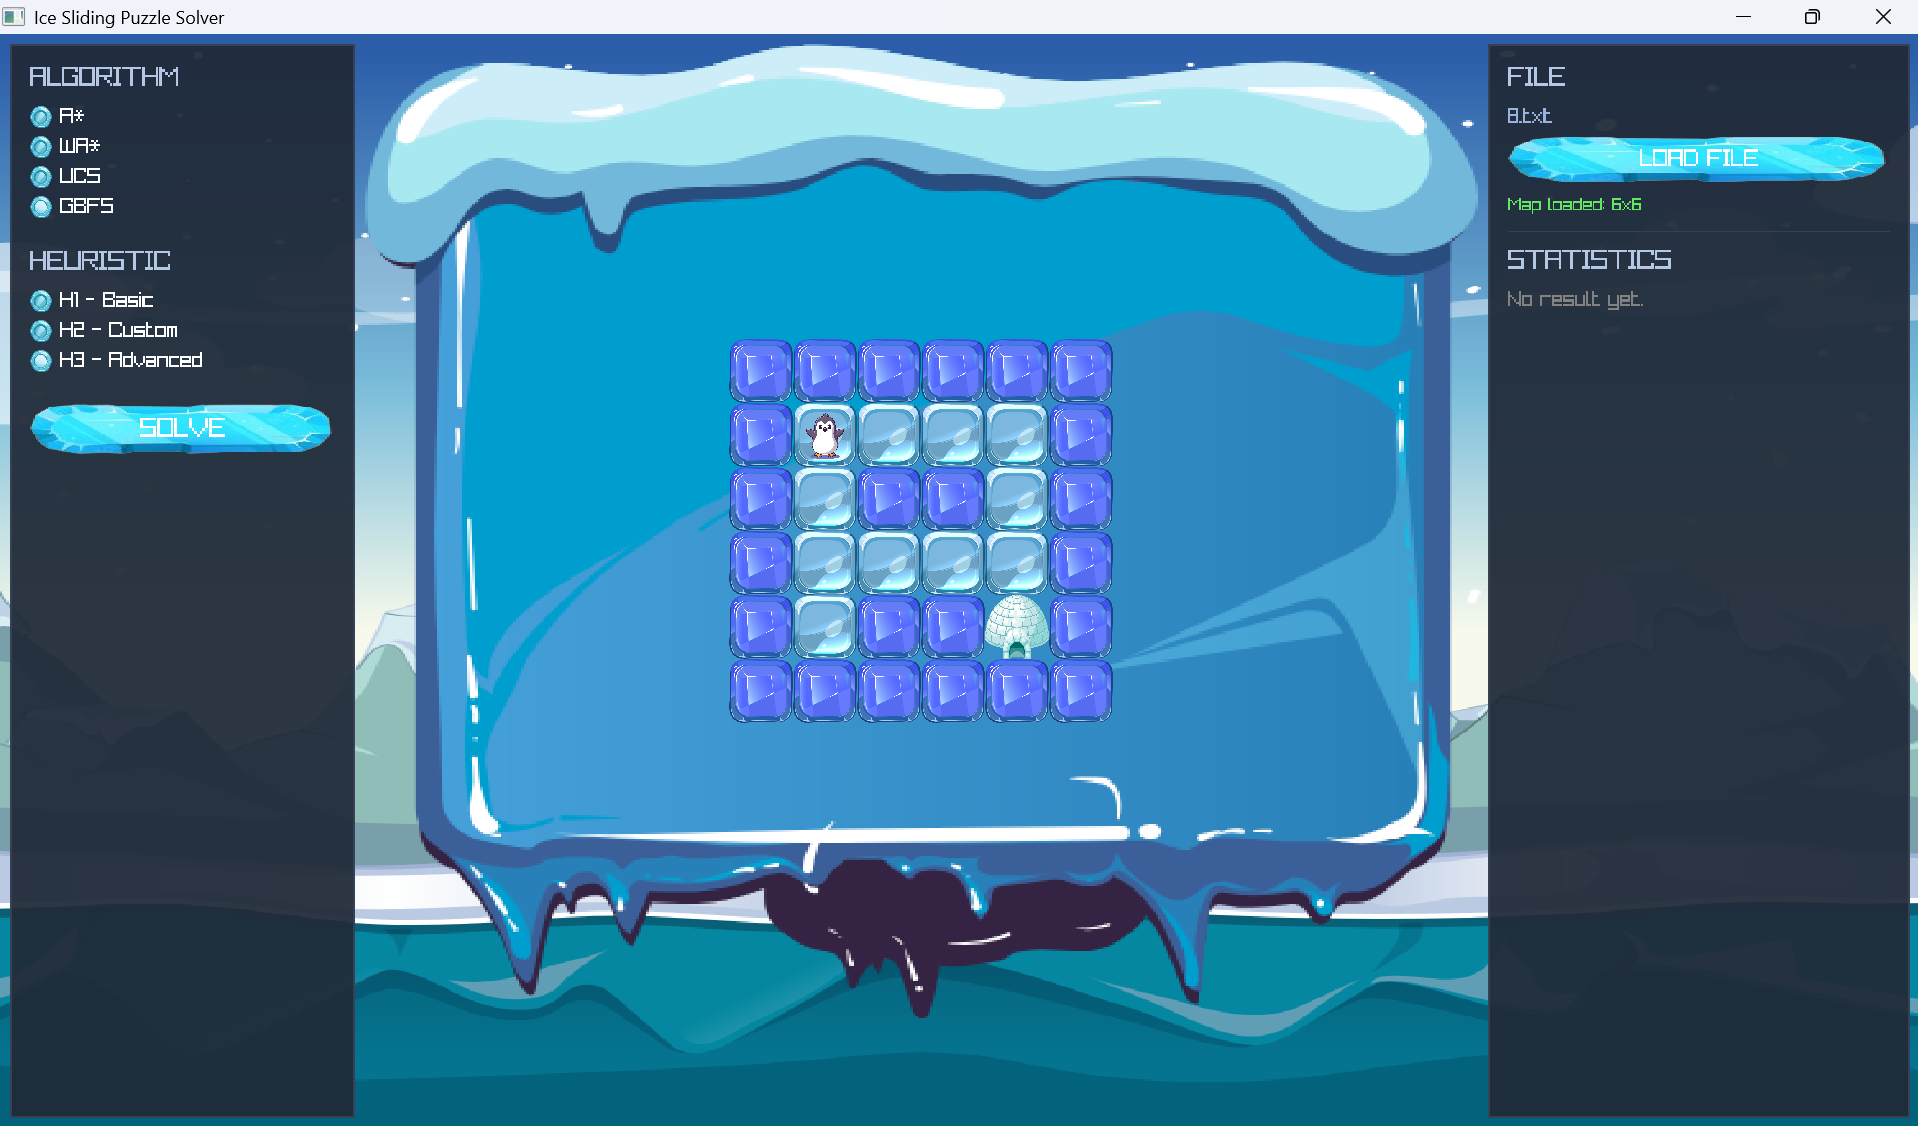
\includegraphics[width=0.55\textwidth]{public/map8.png}
	\caption{Visualisasi map pada Test Case 8}
\end{figure}

\begin{figure}[H]
	\centering
	\begin{minipage}{0.48\textwidth}
		\centering
		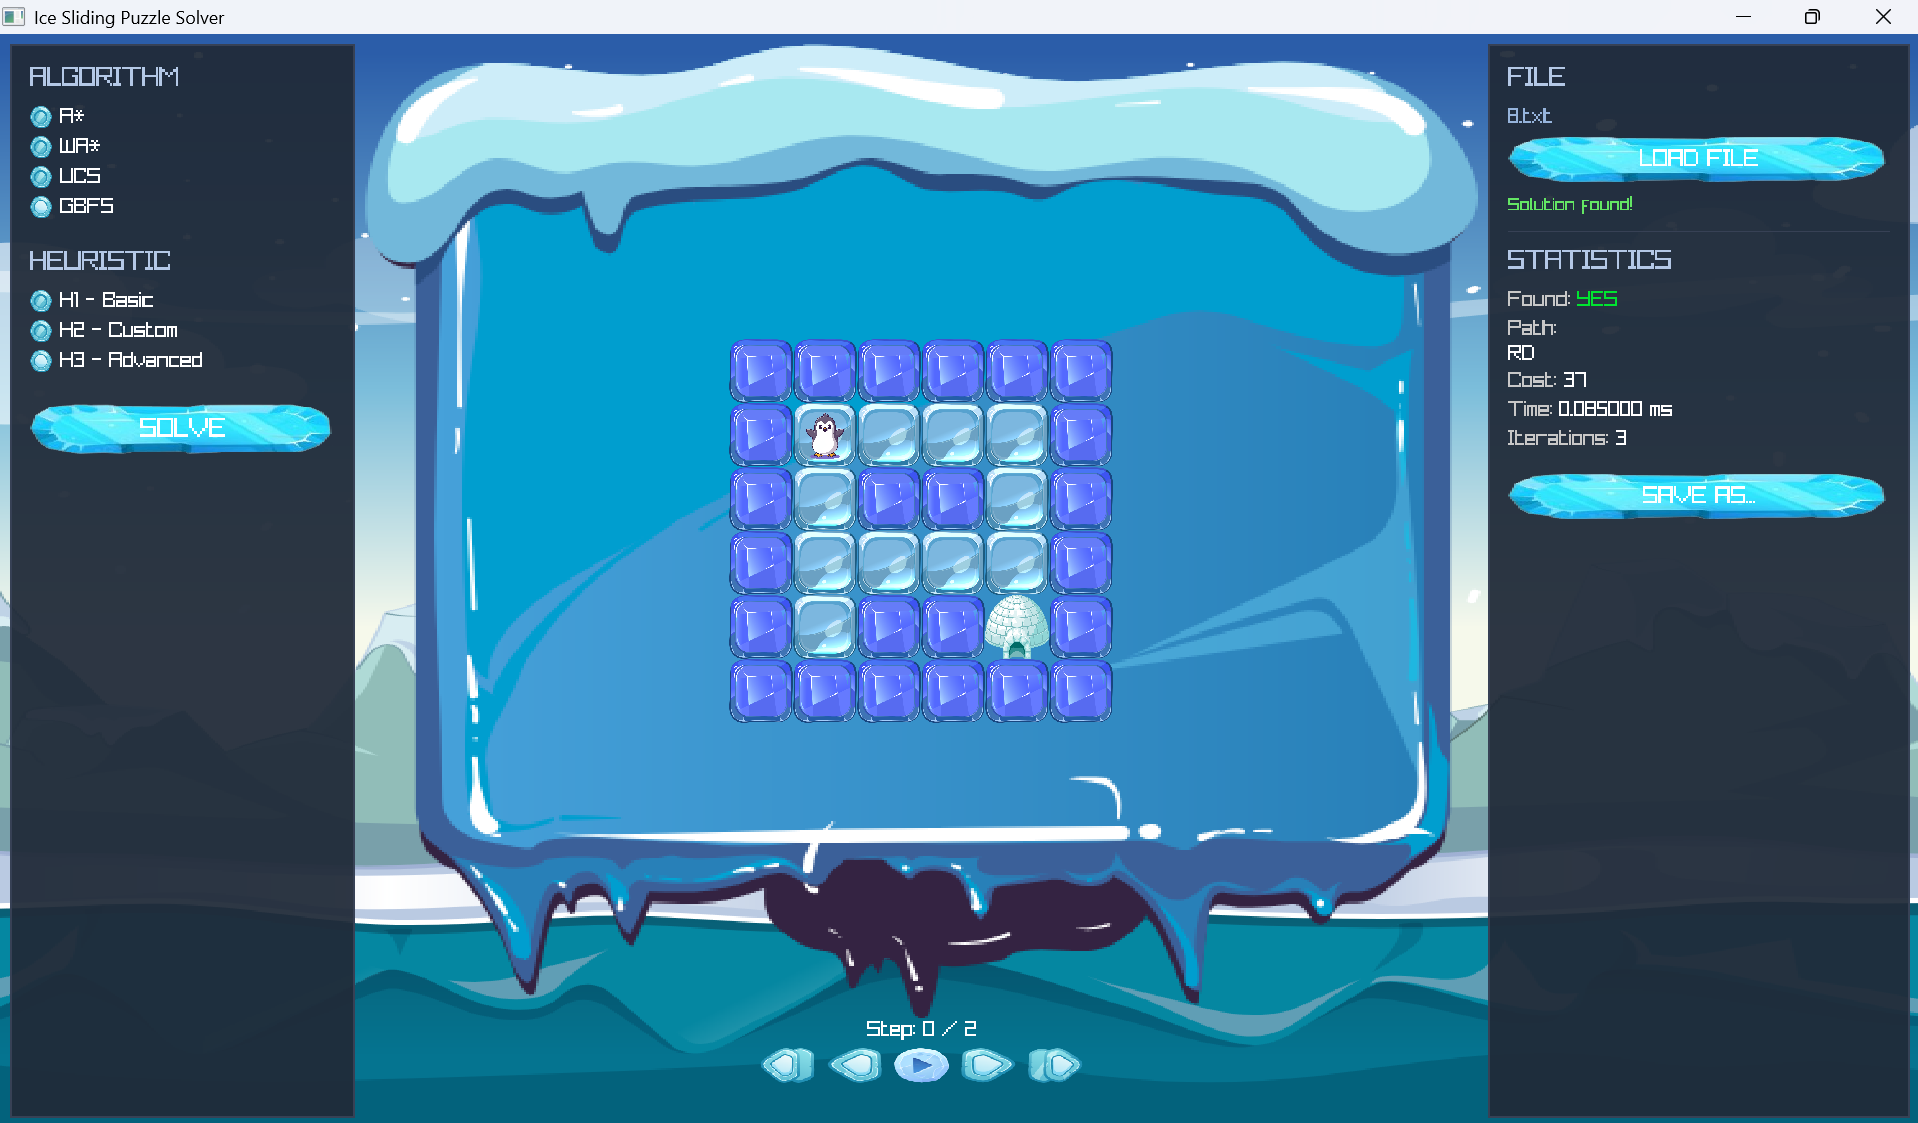
\includegraphics[width=\textwidth]{public/test8-GBFS-h3.png}
		\caption{Output Test 8 menggunakan GBFS + H3}
	\end{minipage}
	\hfill
	\begin{minipage}{0.48\textwidth}
		\centering
		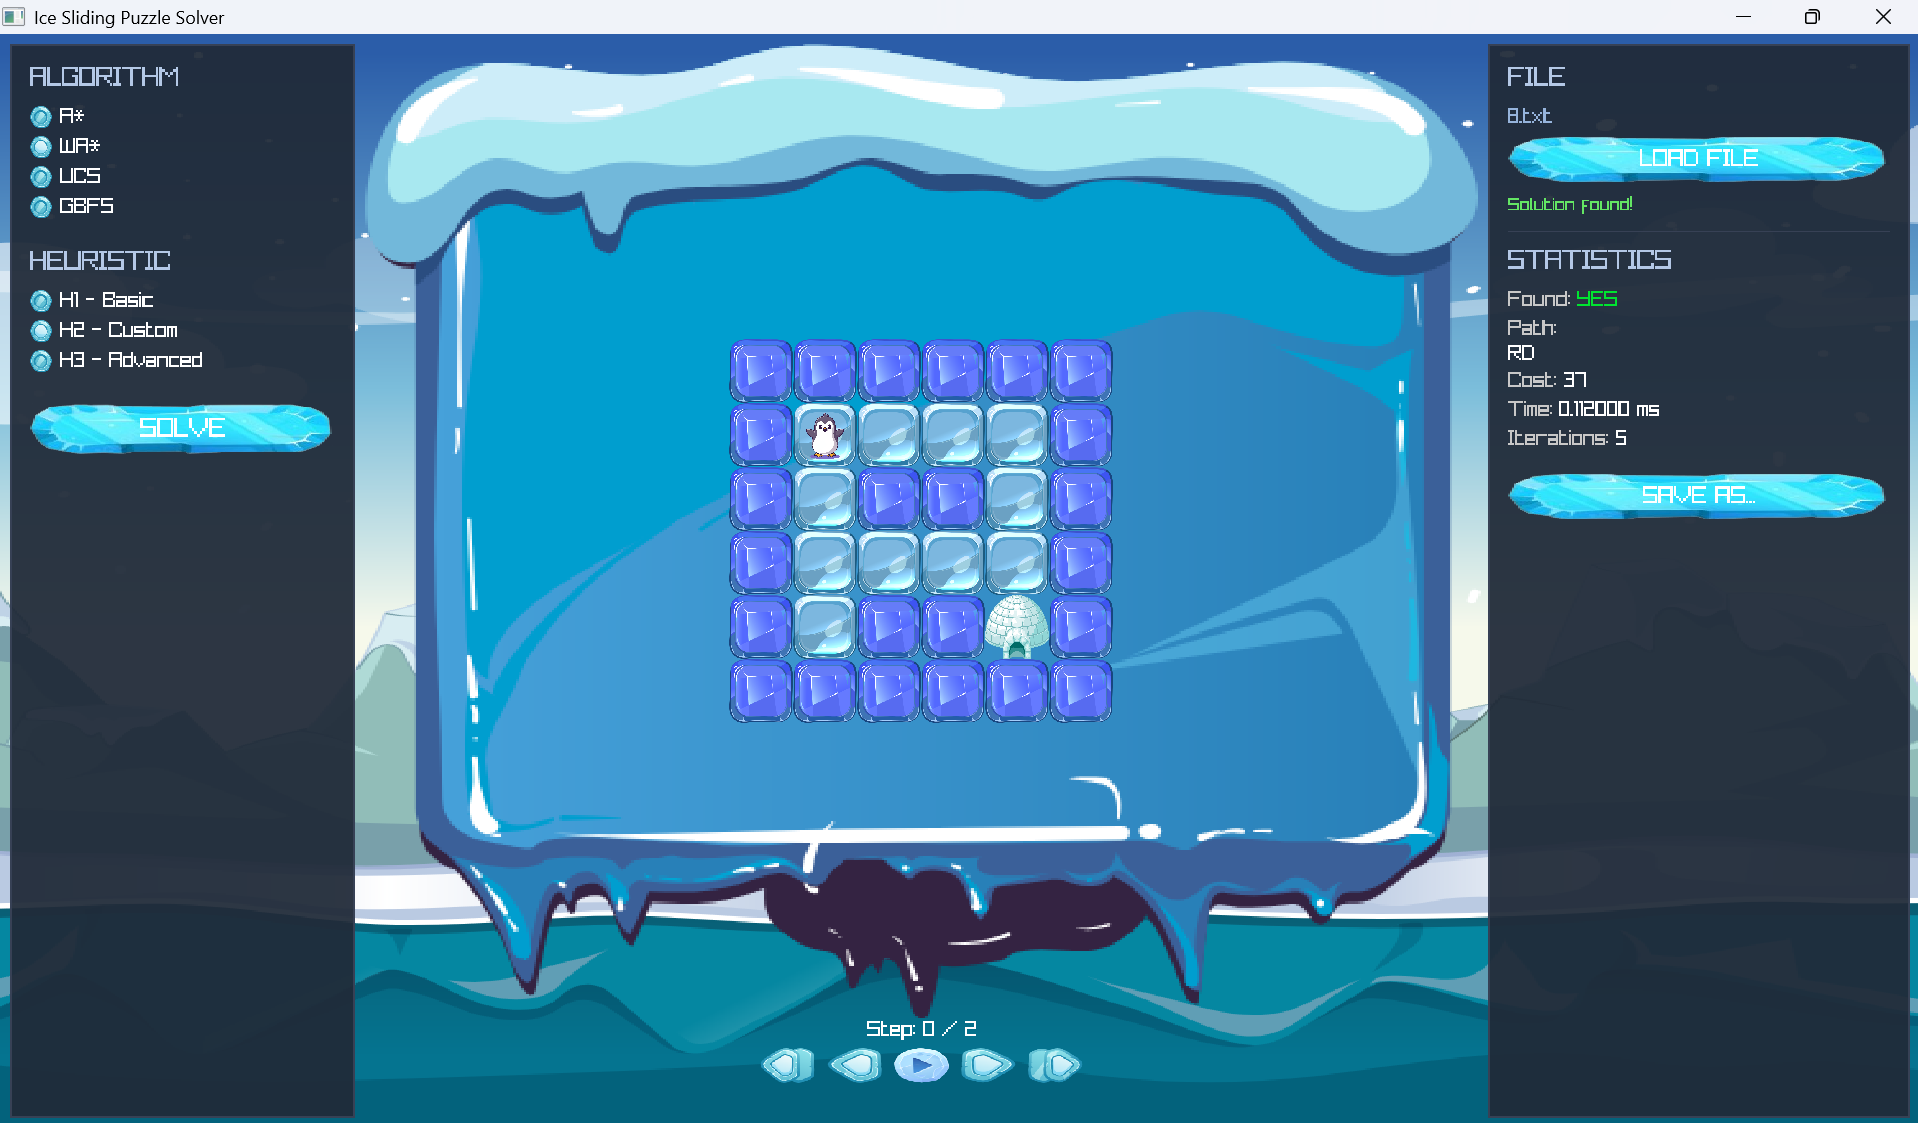
\includegraphics[width=\textwidth]{public/test8-WA-h2.png}
		\caption{Output Test 8 menggunakan Weighted A* + H2}
	\end{minipage}
\end{figure}

\begin{table}[H]
	\centering
	\caption{Hasil percobaan pada Test Case 8}
	\small
	\begin{tabular}{|p{4cm}|p{2.5cm}|p{2.5cm}|p{2.5cm}|}
		\hline
		\rowcolor{gray!20}
		\textbf{Algoritma} & \textbf{Cost} & \textbf{Time (ms)} & \textbf{Iterations} \\
		\hline
		A* - Basic & 37 & 0.124 & 5 \\
		\hline
		A* - Custom & 37 & 0.103 & 5 \\
		\hline
		A* - Advanced & 37 & 0.145 & 5 \\
		\hline
		WA* - Basic & 37 & 0.120 & 5 \\
		\hline
		WA* - Custom & 37 & 0.112 & 5 \\
		\hline
		WA* - Advanced & 37 & 0.120 & 5 \\
		\hline
		UCS & 37 & 0.102 & 4 \\
		\hline
		GBFS - Basic & 37 & 0.077 & 3 \\
		\hline
		GBFS - Custom & 37 & 0.093 & 3 \\
		\hline
		GBFS - Advanced & 37 & 0.085 & 3 \\
		\hline
	\end{tabular}
\end{table}

\begin{tcolorbox}[
	colback=green!5,
	colframe=green!50!black,
	title=\textbf{Ringkasan Test Case 8},
	arc=2mm,
	boxrule=0.8pt
]
Seluruh algoritma menghasilkan cost solusi yang sama, yaitu 37. 
Hal ini menunjukkan bahwa pada map sederhana tanpa angka dan lava, perbedaan algoritma lebih terlihat pada jumlah iterasi dan waktu eksekusi, bukan pada kualitas cost solusi.
\end{tcolorbox}


\subsection{Test Case 17}

\begin{tcolorbox}[
	colback=blue!5,
	colframe=blue!60!black,
	title=\textbf{Ringkasan Input Test Case 17},
	arc=2mm,
	boxrule=0.8pt
]
Test case 17 menggunakan papan berukuran $10 \times 10$ dengan banyak angka wajib dari \texttt{0} sampai \texttt{7}. 
Kasus ini digunakan untuk menguji kemampuan algoritma dalam mengikuti constraint angka berurutan sambil tetap memperhitungkan cost tile yang bervariasi.
\end{tcolorbox}

\begin{table}[H]
	\centering
	\caption{Karakteristik input Test Case 17}
	\begin{tabular}{|p{4cm}|p{9.5cm}|}
		\hline
		\rowcolor{blue!15}
		\textbf{Aspek} & \textbf{Keterangan} \\
		\hline
		Ukuran papan & $10 \times 10$ \\
		\hline
		Posisi awal & Ditandai dengan karakter \texttt{Z} pada bagian bawah map \\
		\hline
		Goal & Ditandai dengan karakter \texttt{O} \\
		\hline
		Angka wajib & Terdapat angka \texttt{0} sampai \texttt{7} yang harus dilalui berurutan \\
		\hline
		Lava & Tidak ada \\
		\hline
		Karakteristik utama & Map berisi banyak angka dan cost tile yang meningkat, sehingga cocok untuk menguji perbedaan cost solusi dan jumlah iterasi. \\
		\hline
	\end{tabular}
\end{table}

\begin{tcolorbox}[
	colback=gray!5,
	colframe=black!60,
	title=\textbf{Isi File \texttt{17.txt}},
	arc=2mm,
	boxrule=0.8pt
]
\tiny
\begin{verbatim}
10 10
XXXXXXXXXX
X***X****X
X*****3*XX
X********X
X***2**4*X
XX***5***X
X**1*X*X*X
X06******X
XZ***7*OXX
XXXXXXXXXX
999 999 999 999 999 999 999 999 999 999
999 5 2 3 999 6 7 8 9 999
999 1 10 11 12 13 14 15 999 999
999 17 18 19 20 21 22 23 24 999
999 25 26 27 28 29 30 31 32 999
999 999 34 35 36 37 38 39 40 999
999 41 42 43 44 999 46 999 48 999
999 49 50 51 52 53 54 55 56 999
999 57 58 59 60 61 62 63 999 999
999 999 999 999 999 999 999 999 999 999
\end{verbatim}
\end{tcolorbox}

\begin{figure}[H]
	\centering
	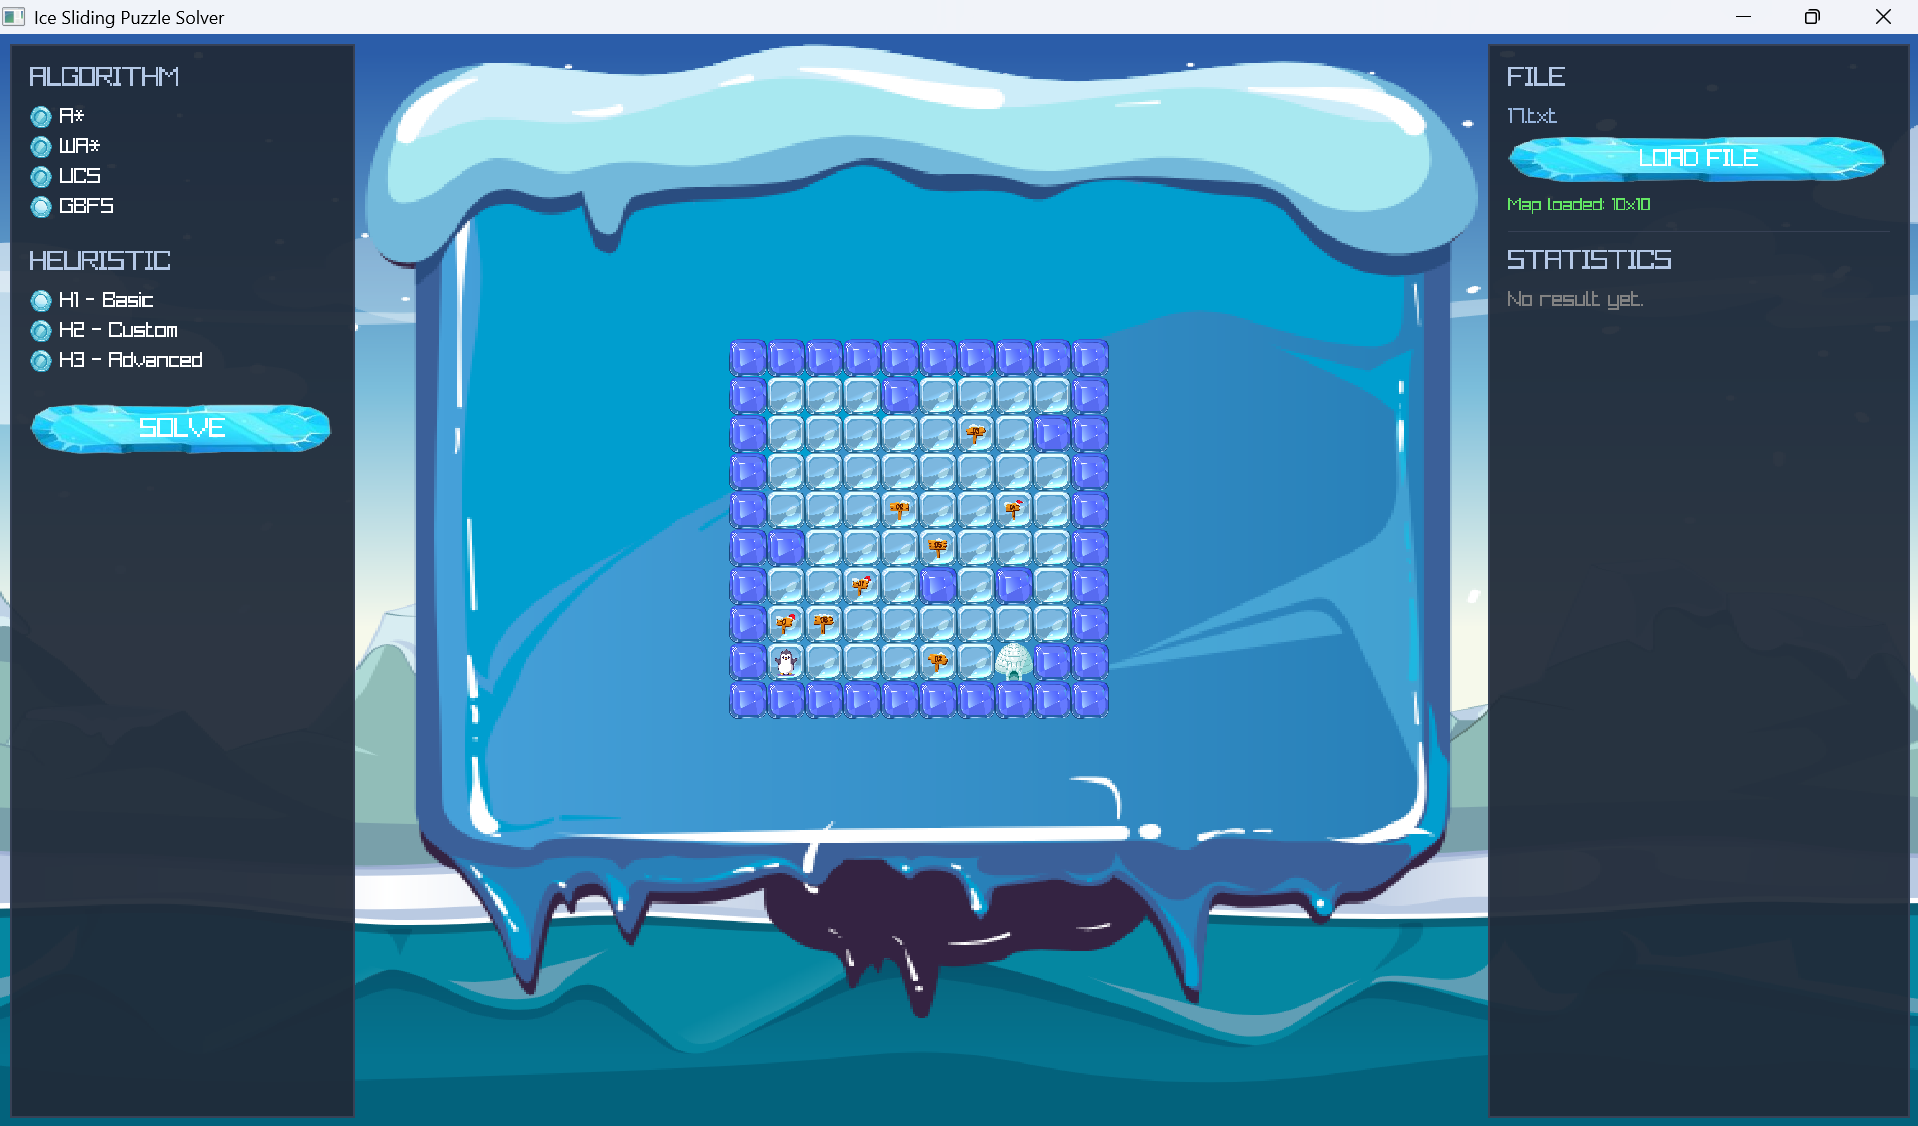
\includegraphics[width=0.65\textwidth]{public/map17.png}
	\caption{Visualisasi map pada Test Case 17}
\end{figure}

\begin{figure}[H]
	\centering
	\begin{minipage}{0.48\textwidth}
		\centering
		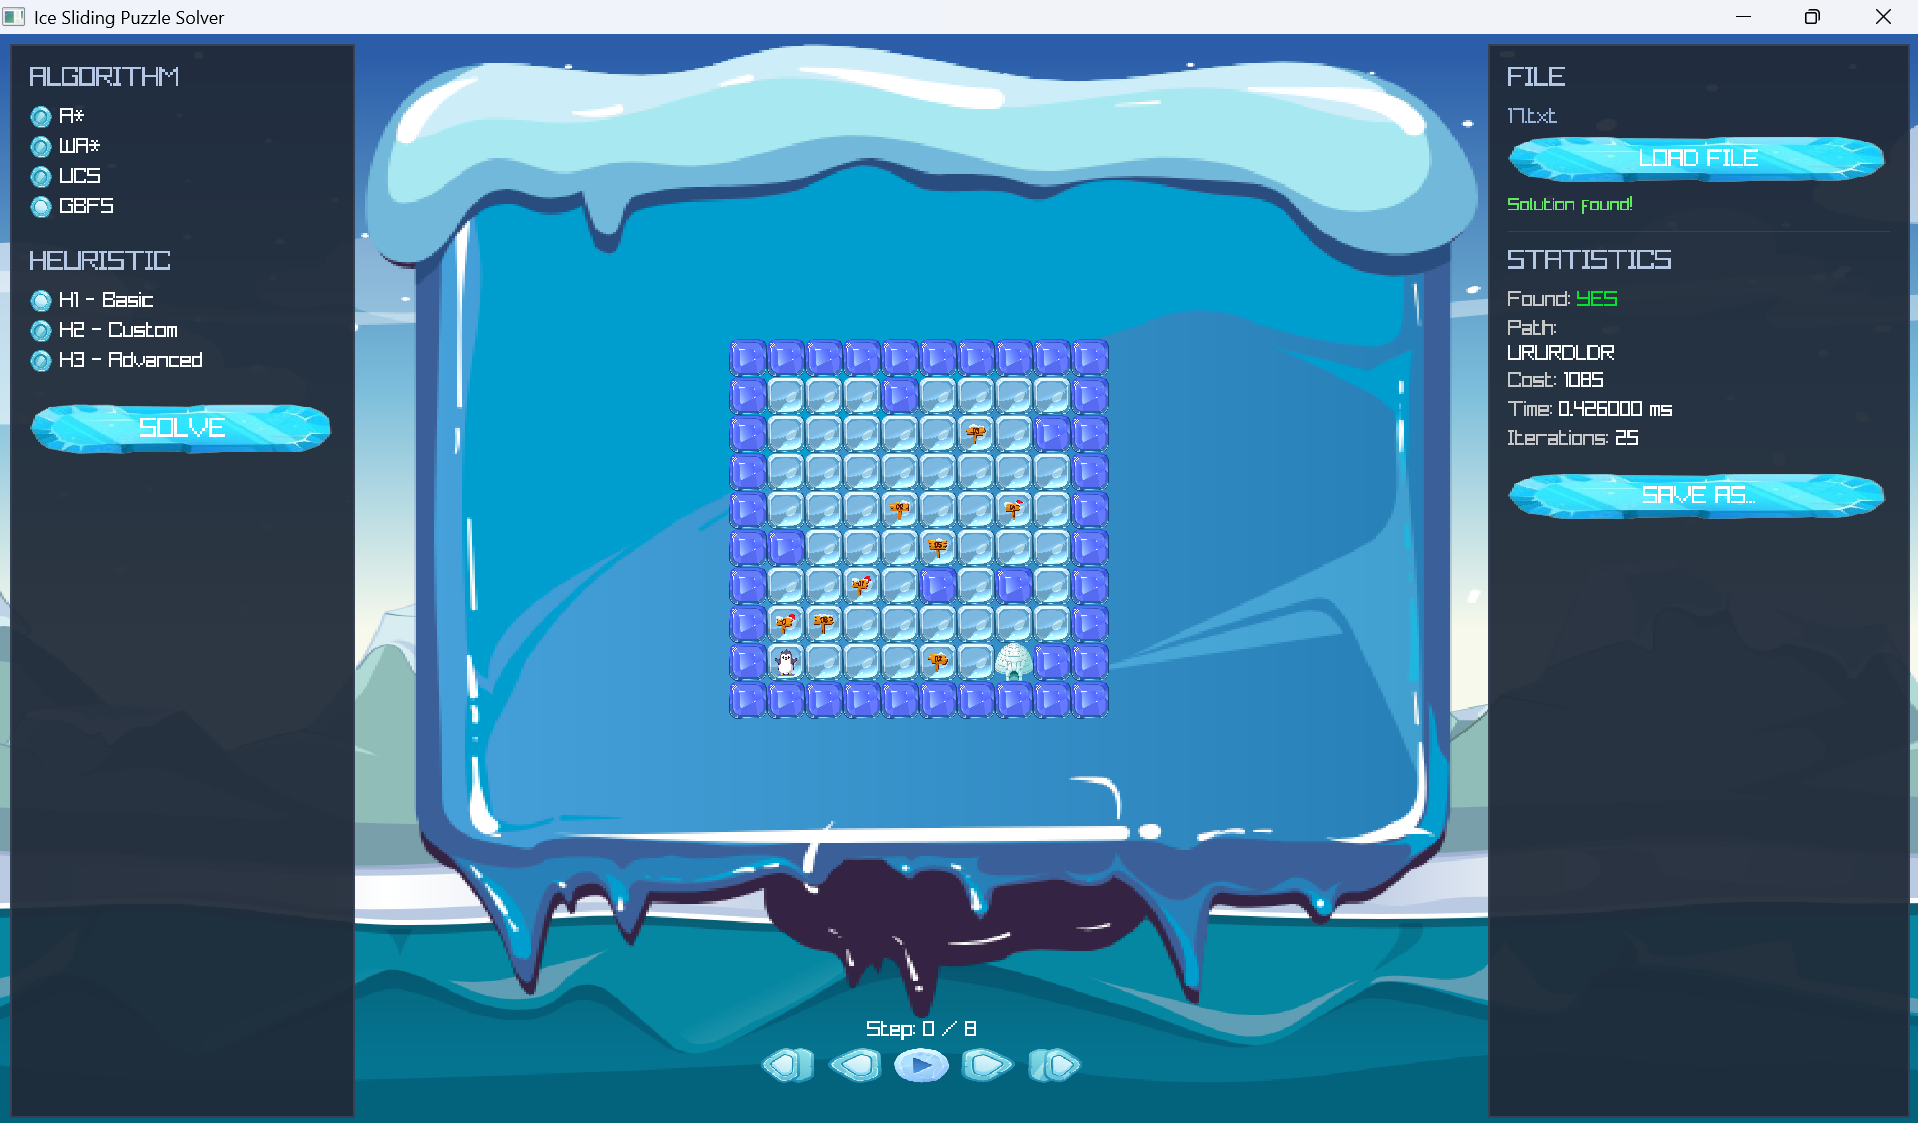
\includegraphics[width=\textwidth]{public/test17-GBFS-h1.png}
		\caption{Output Test 17 menggunakan GBFS + H1}
	\end{minipage}
	\hfill
	\begin{minipage}{0.48\textwidth}
		\centering
		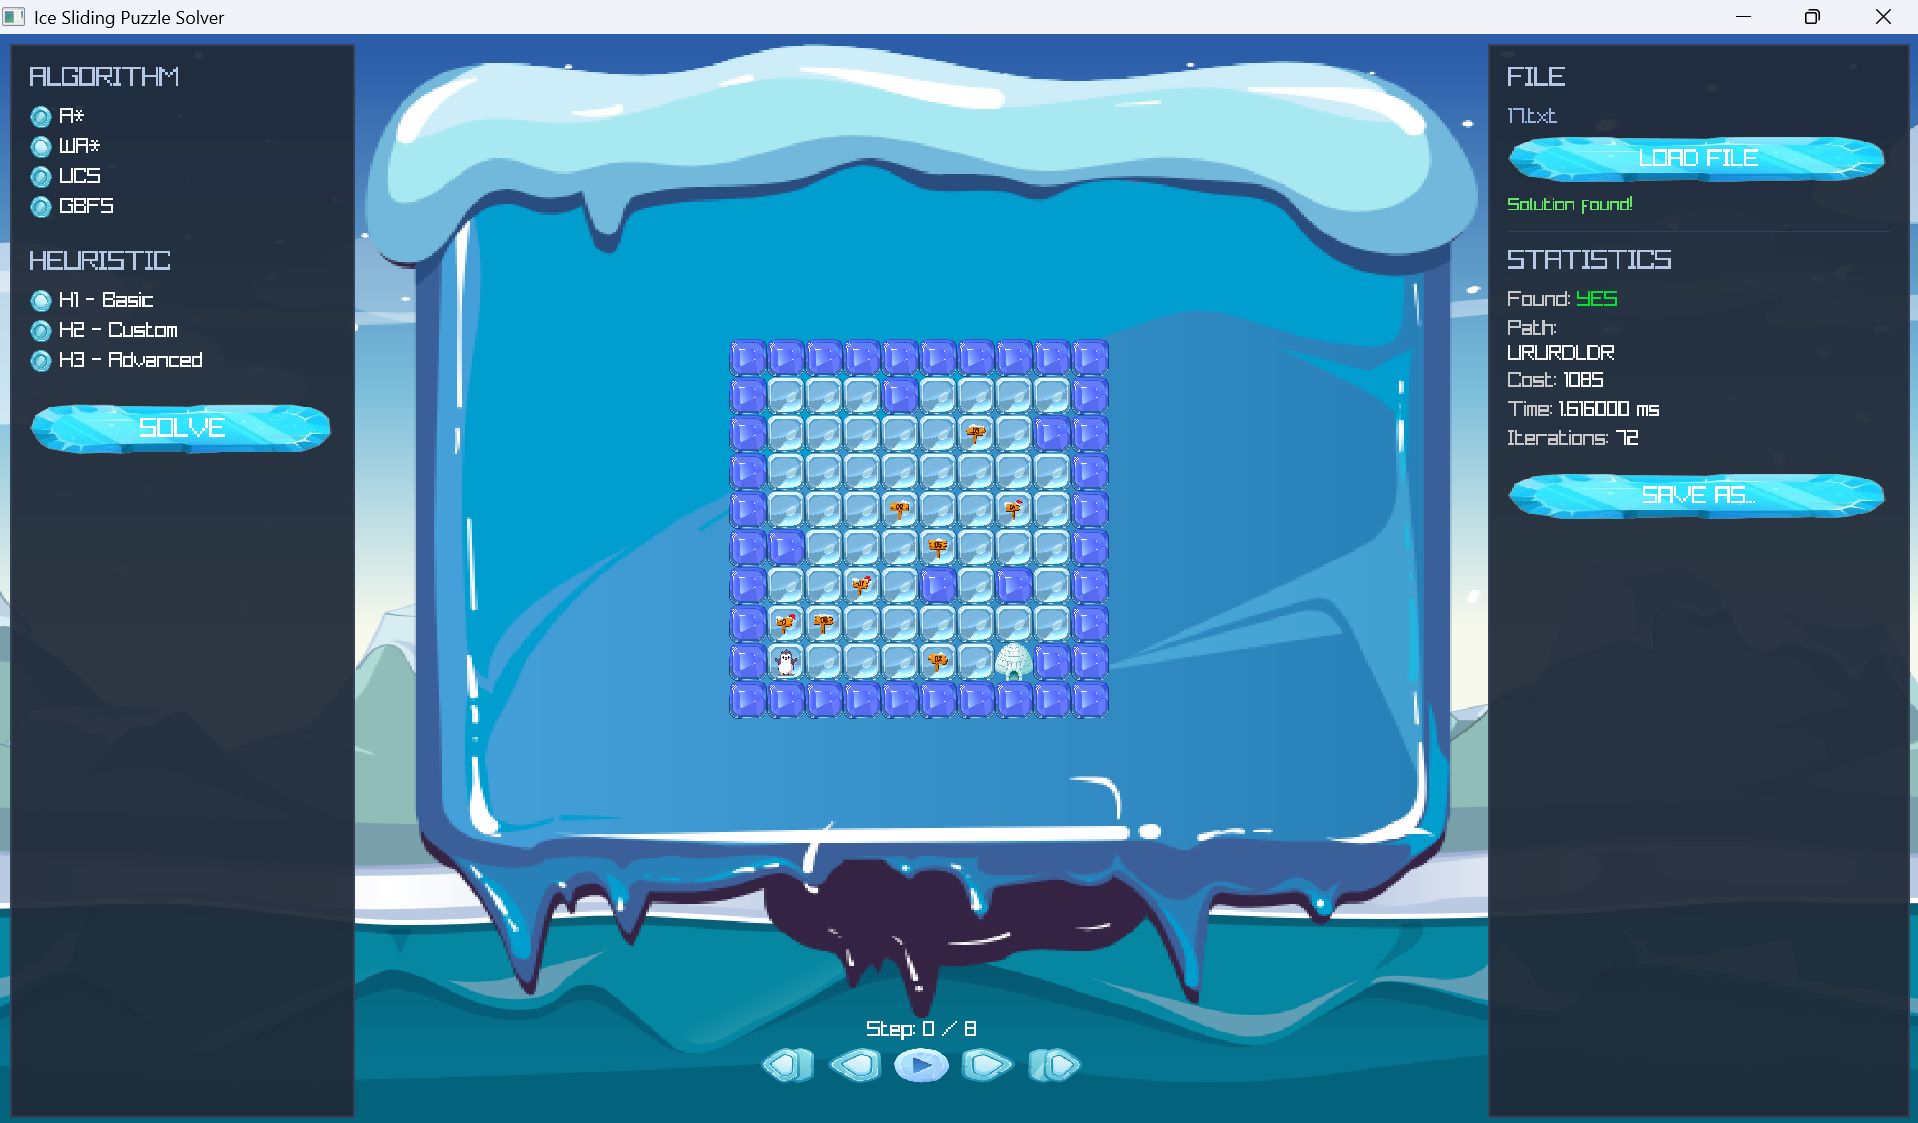
\includegraphics[width=\textwidth]{public/test17-WA-h1.png}
		\caption{Output Test 17 menggunakan Weighted A* + H1}
	\end{minipage}
\end{figure}

\begin{table}[H]
	\centering
	\caption{Hasil percobaan pada Test Case 17}
	\small
	\begin{tabular}{|p{4cm}|p{2.5cm}|p{2.5cm}|p{2.5cm}|}
		\hline
		\rowcolor{gray!20}
		\textbf{Algoritma} & \textbf{Cost} & \textbf{Time (ms)} & \textbf{Iterations} \\
		\hline
		A* - Basic & 1085 & 1.741 & 72 \\
		\hline
		A* - Custom & 1085 & 1.796 & 72 \\
		\hline
		A* - Advanced & 1085 & 2.639 & 72 \\
		\hline
		WA* - Basic & 1085 & 1.616 & 72 \\
		\hline
		WA* - Custom & 1085 & 2.232 & 72 \\
		\hline
		WA* - Advanced & 1085 & 2.581 & 72 \\
		\hline
		UCS & 1085 & 1.228 & 71 \\
		\hline
		GBFS - Basic & 1085 & 0.552 & 25 \\
		\hline
		GBFS - Custom & 1085 & 0.439 & 11 \\
		\hline
		GBFS - Advanced & 1085 & 0.534 & 10 \\
		\hline
	\end{tabular}
\end{table}

\begin{tcolorbox}[
	colback=green!5,
	colframe=green!50!black,
	title=\textbf{Ringkasan Test Case 17},
	arc=2mm,
	boxrule=0.8pt
]
Semua algoritma menghasilkan cost solusi yang sama, yaitu 1085. 
Namun, GBFS dengan heuristik Custom dan Advanced meninjau jumlah iterasi yang jauh lebih sedikit dibanding UCS, A*, dan Weighted A*. 
Hal ini menunjukkan bahwa pada map ini, heuristik mampu mengarahkan pencarian secara efektif.
\end{tcolorbox}


\subsection{Test Case 20}

\begin{tcolorbox}[
	colback=blue!5,
	colframe=blue!60!black,
	title=\textbf{Ringkasan Input Test Case 20},
	arc=2mm,
	boxrule=0.8pt
]
Test case 20 menggunakan papan berukuran $12 \times 12$ dengan pola obstacle yang menyerupai labirin. 
Tidak terdapat angka wajib maupun lava, sehingga pengujian difokuskan pada kemampuan algoritma mencari lintasan sliding yang valid di antara banyak rintangan.
\end{tcolorbox}

\begin{table}[H]
	\centering
	\caption{Karakteristik input Test Case 20}
	\begin{tabular}{|p{4cm}|p{9.5cm}|}
		\hline
		\rowcolor{blue!15}
		\textbf{Aspek} & \textbf{Keterangan} \\
		\hline
		Ukuran papan & $12 \times 12$ \\
		\hline
		Posisi awal & Ditandai dengan karakter \texttt{Z} pada kiri atas area bebas \\
		\hline
		Goal & Ditandai dengan karakter \texttt{O} pada kanan bawah area bebas \\
		\hline
		Angka wajib & Tidak ada \\
		\hline
		Lava & Tidak ada \\
		\hline
		Karakteristik utama & Map labirin dengan banyak obstacle, sehingga menguji kemampuan algoritma menemukan jalur sliding yang tidak langsung. \\
		\hline
	\end{tabular}
\end{table}

\begin{tcolorbox}[
	colback=gray!5,
	colframe=black!60,
	title=\textbf{Isi File \texttt{20.txt}},
	arc=2mm,
	boxrule=0.8pt
]
\tiny
\begin{verbatim}
12 12
XXXXXXXXXXXX
XZ*********X
X*XXXXXXXX*X
X*X******X*X
X*X*XXXX*X*X
X*X*X**X*X*X
X*X*X**X*X*X
X*X*XXXX*X*X
X*X******X*X
X*XXXXXXXX*X
X*********OX
XXXXXXXXXXXX
999 999 999 999 999 999 999 999 999 999 999 999
999 1 2 3 4 5 6 7 8 9 10 999
999 11 999 999 999 999 999 999 999 999 12 999
999 13 999 14 15 16 17 18 19 20 999 999
999 21 999 22 999 999 23 24 999 25 999 999
999 26 999 27 999 28 29 999 30 31 999 999
999 32 999 33 999 34 35 999 36 37 999 999
999 38 999 39 999 999 40 41 999 42 999 999
999 43 999 44 45 46 47 48 49 50 999 999
999 51 999 999 999 999 999 999 999 999 52 999
999 53 54 55 56 57 58 59 60 61 62 999
999 999 999 999 999 999 999 999 999 999 999 999
\end{verbatim}
\end{tcolorbox}

\begin{figure}[H]
	\centering
	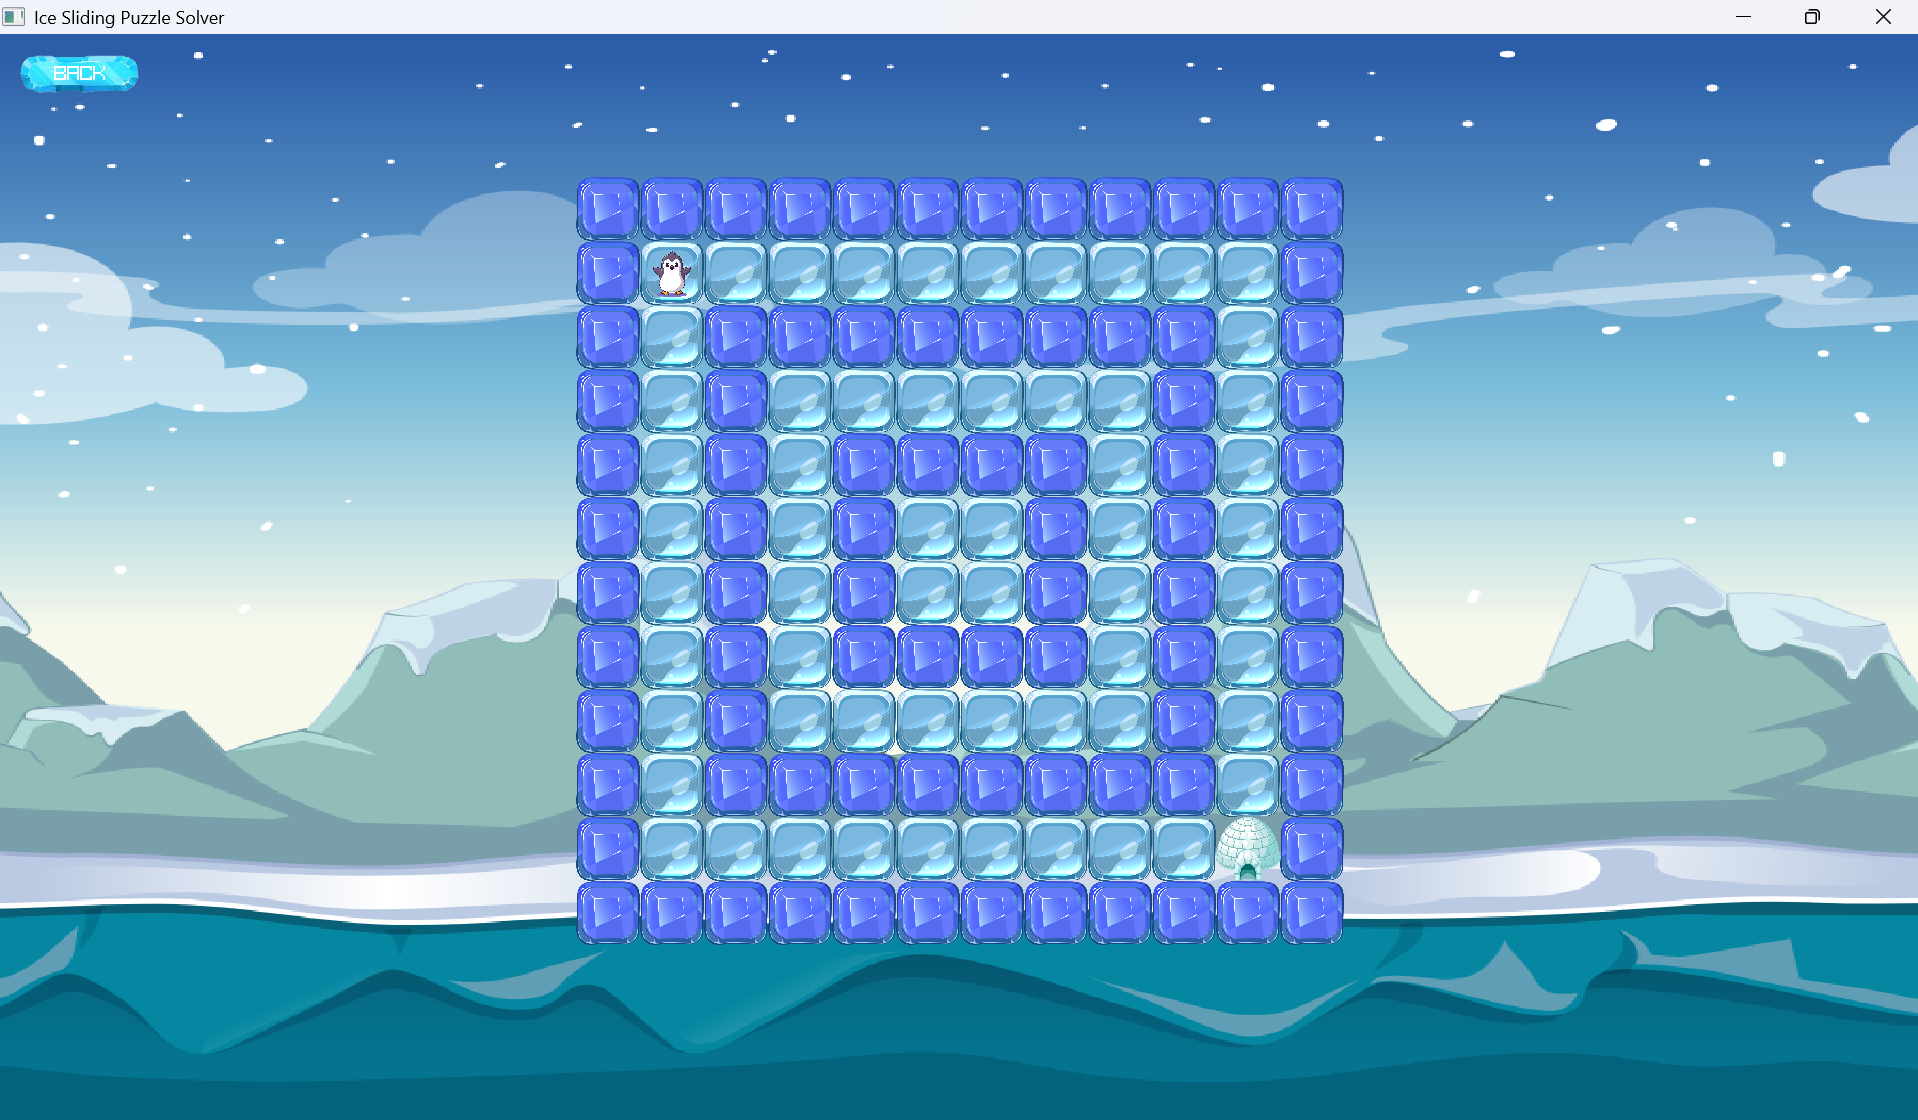
\includegraphics[width=0.65\textwidth]{public/map-20.png}
	\caption{Visualisasi map pada Test Case 20}
\end{figure}

\begin{figure}[H]
	\centering
	\begin{minipage}{0.48\textwidth}
		\centering
		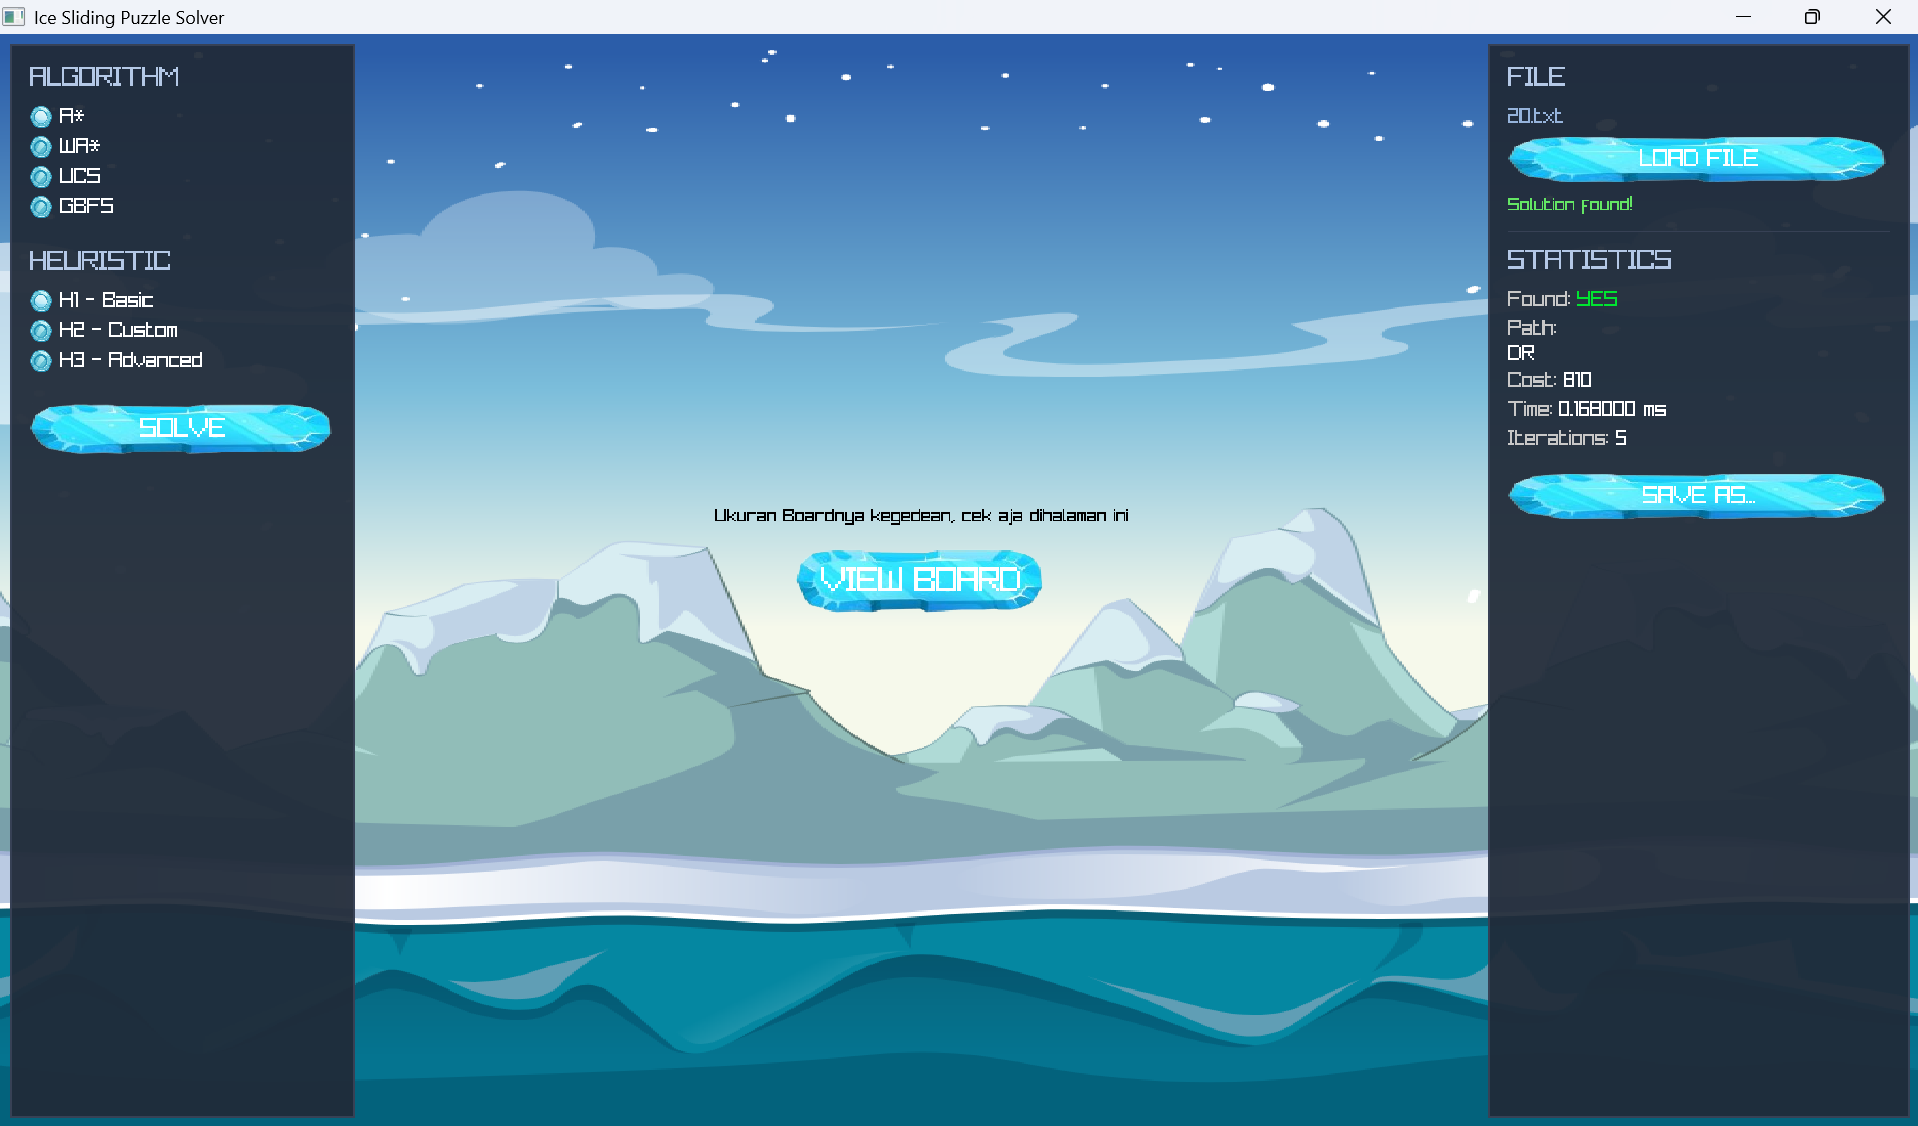
\includegraphics[width=\textwidth]{public/test20-A-h1.png}
		\caption{Output Test 20 menggunakan A* + H1}
	\end{minipage}
	\hfill
	\begin{minipage}{0.48\textwidth}
		\centering
		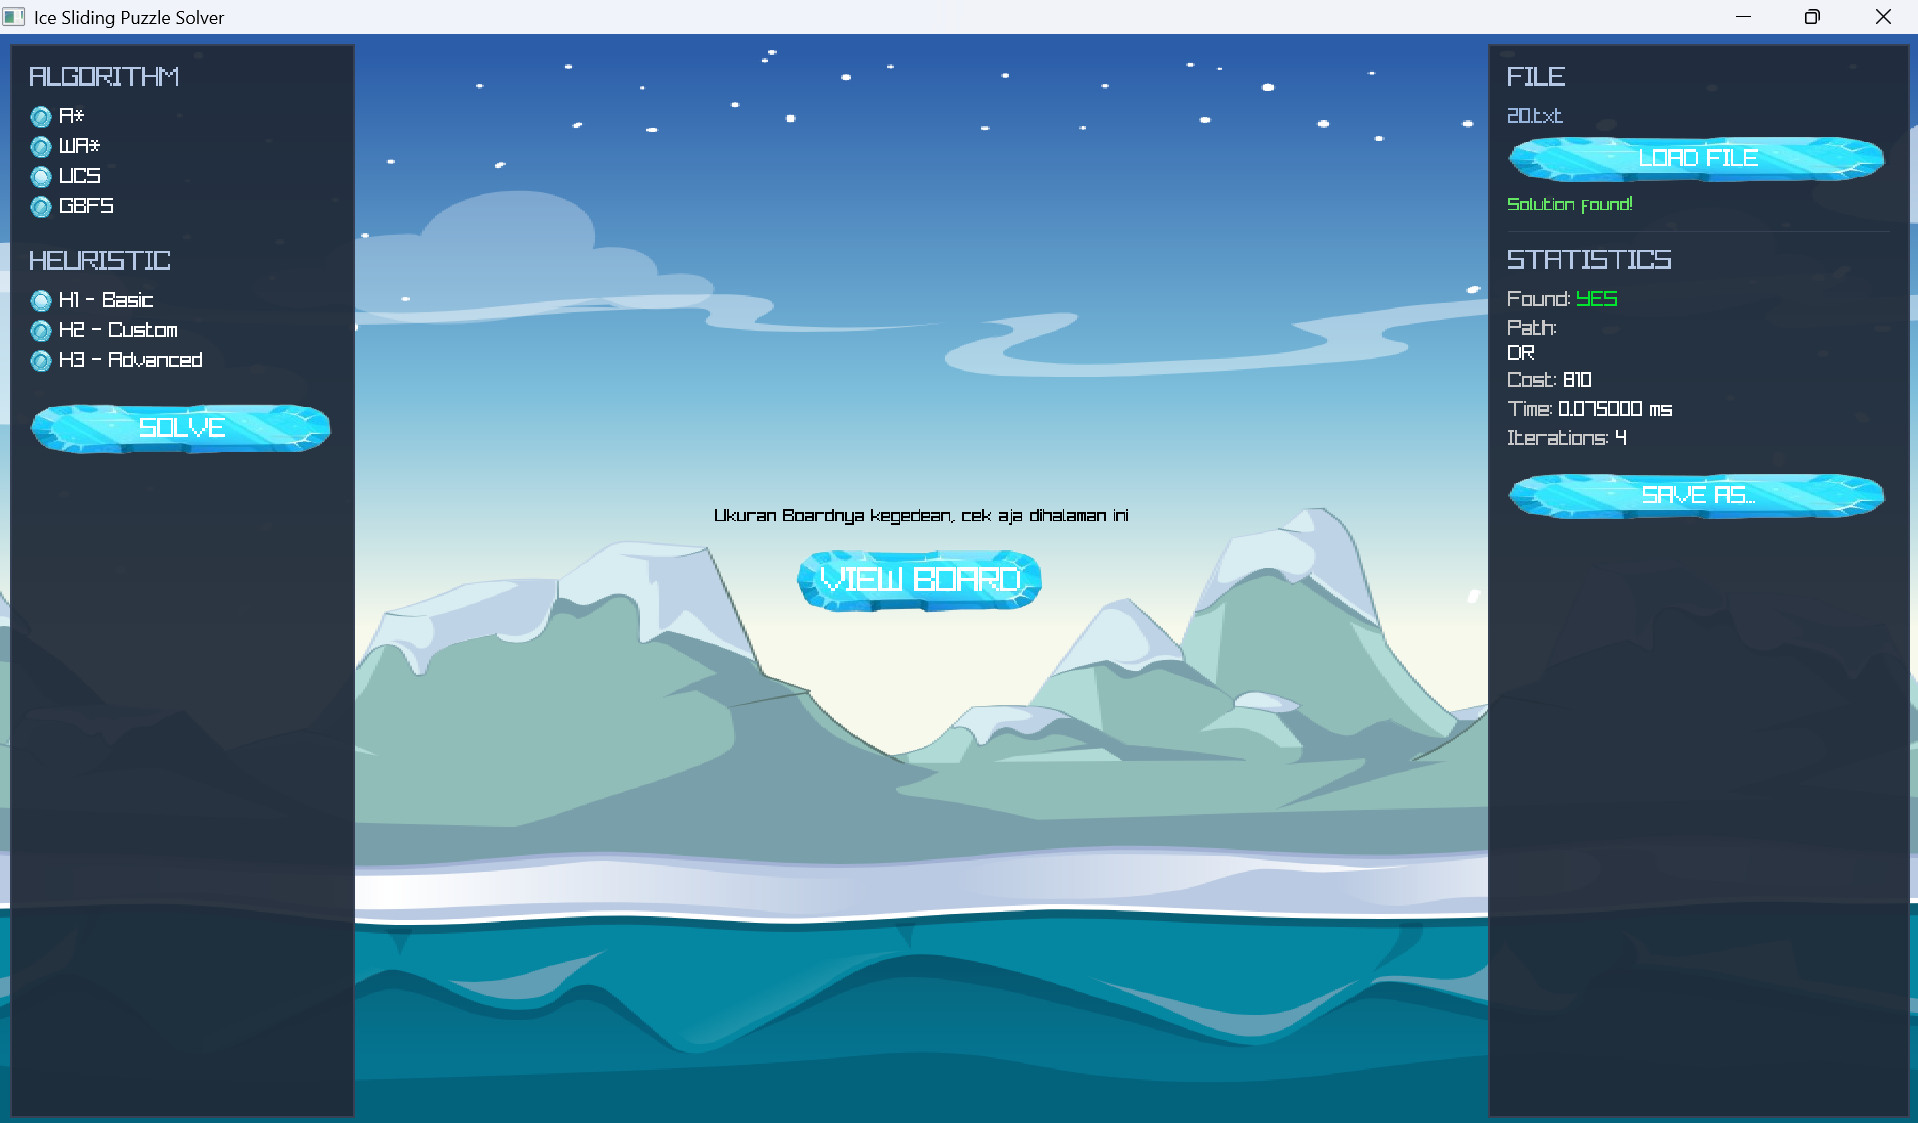
\includegraphics[width=\textwidth]{public/test20-UCS.png}
		\caption{Output Test 20 menggunakan UCS}
	\end{minipage}
\end{figure}

\begin{table}[H]
	\centering
	\caption{Hasil percobaan pada Test Case 20}
	\small
	\begin{tabular}{|p{4cm}|p{2.5cm}|p{2.5cm}|p{2.5cm}|}
		\hline
		\rowcolor{gray!20}
		\textbf{Algoritma} & \textbf{Cost} & \textbf{Time (ms)} & \textbf{Iterations} \\
		\hline
		A* - Basic & 810 & 0.196 & 5 \\
		\hline
		A* - Custom & 810 & 0.250 & 5 \\
		\hline
		A* - Advanced & 810 & 0.203 & 5 \\
		\hline
		WA* - Basic & 810 & 0.110 & 5 \\
		\hline
		WA* - Custom & 810 & 0.380 & 5 \\
		\hline
		WA* - Advanced & 810 & 0.246 & 5 \\
		\hline
		UCS & 810 & 0.113 & 4 \\
		\hline
		GBFS - Basic & 6174 & 0.065 & 3 \\
		\hline
		GBFS - Custom & 6174 & 0.136 & 3 \\
		\hline
		GBFS - Advanced & 6174 & 0.132 & 3 \\
		\hline
	\end{tabular}
\end{table}

\begin{tcolorbox}[
	colback=orange!5,
	colframe=orange!70!black,
	title=\textbf{Ringkasan Test Case 20},
	arc=2mm,
	boxrule=0.8pt
]
Pada test case ini, UCS, A*, dan Weighted A* menghasilkan cost 810, sedangkan GBFS menghasilkan cost 6174. 
Hal ini menunjukkan bahwa GBFS dapat menemukan solusi lebih cepat dari sisi iterasi, tetapi tidak selalu menghasilkan cost minimum karena hanya mengikuti estimasi heuristik.
\end{tcolorbox}


\subsection{Test Case 24}

\begin{tcolorbox}[
	colback=blue!5,
	colframe=blue!60!black,
	title=\textbf{Ringkasan Input Test Case 24},
	arc=2mm,
	boxrule=0.8pt
]
Test case 24 menggunakan papan berukuran $7 \times 12$ yang memiliki angka wajib dan beberapa lava. 
Kasus ini menguji dua aturan penting sekaligus, yaitu angka harus dilewati secara berurutan dan jalur yang melewati lava harus dianggap tidak valid.
\end{tcolorbox}

\begin{table}[H]
	\centering
	\caption{Karakteristik input Test Case 24}
	\begin{tabular}{|p{4cm}|p{9.5cm}|}
		\hline
		\rowcolor{blue!15}
		\textbf{Aspek} & \textbf{Keterangan} \\
		\hline
		Ukuran papan & $7 \times 12$ \\
		\hline
		Posisi awal & Ditandai dengan karakter \texttt{Z} pada sisi kiri map \\
		\hline
		Goal & Ditandai dengan karakter \texttt{O} pada sisi kanan bawah map \\
		\hline
		Angka wajib & Terdapat angka \texttt{0} sampai \texttt{6} yang harus dilalui berurutan \\
		\hline
		Lava & Ada beberapa tile \texttt{L} yang menyebabkan game over jika dilewati \\
		\hline
		Karakteristik utama & Kombinasi angka, obstacle, dan lava sehingga cocok untuk menguji validasi path dan constraint urutan angka. \\
		\hline
	\end{tabular}
\end{table}

\begin{tcolorbox}[
	colback=gray!5,
	colframe=black!60,
	title=\textbf{Isi File \texttt{24.txt}},
	arc=2mm,
	boxrule=0.8pt
]
\tiny
\begin{verbatim}
7 12
XXXXXXXXXXXX
XZ01*******X
X**L**X*L**X
X****4**3*2X
X5*X***L**XX
X***6*****OX
XXXXXXXXXXXX
999 999 999 999 999 999 999 999 999 999 999 999
999 1 2 3 4 5 6 7 8 9 10 999
999 11 12 999 13 14 999 15 999 16 17 999
999 18 19 20 21 22 23 24 25 26 27 999
999 28 29 999 30 31 32 999 33 34 999 999
999 35 36 37 38 39 40 41 42 43 44 999
999 999 999 999 999 999 999 999 999 999 999 999
\end{verbatim}
\end{tcolorbox}

\begin{figure}[H]
	\centering
	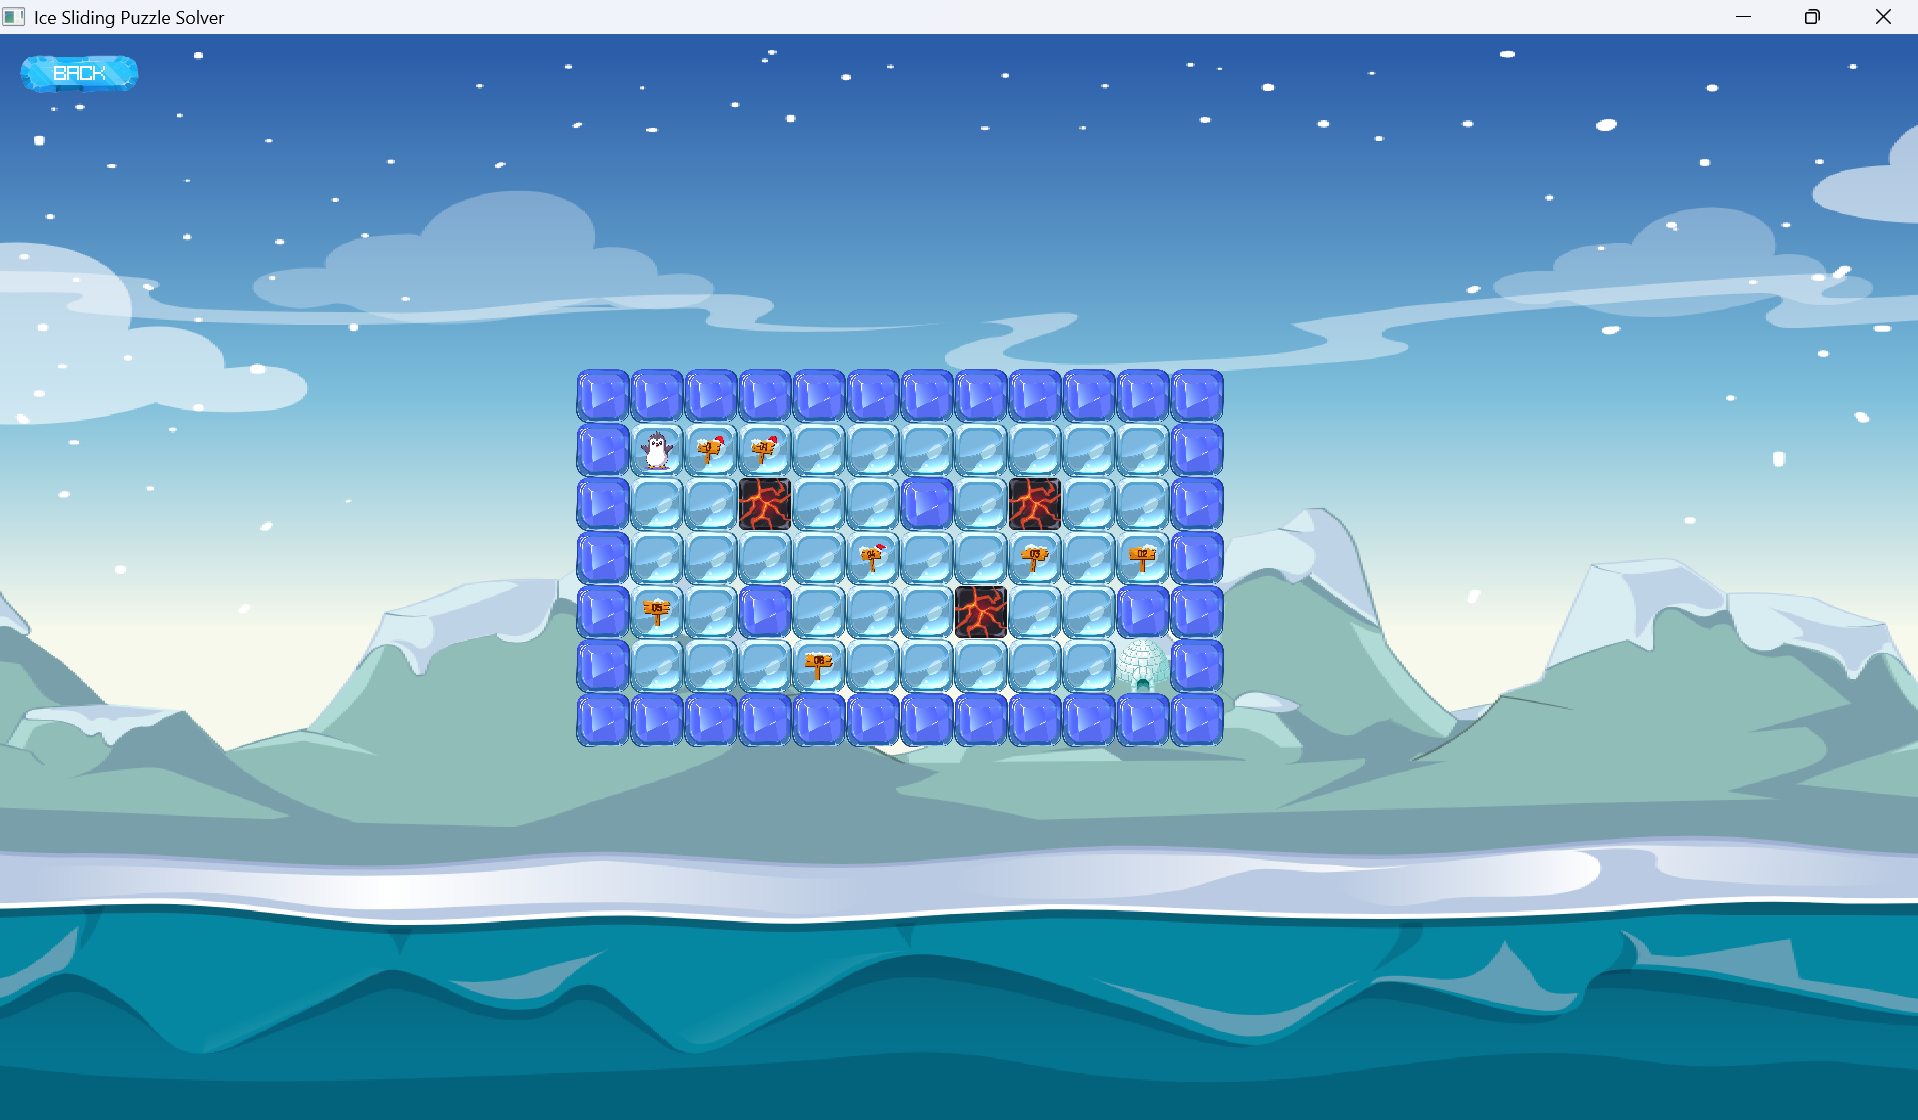
\includegraphics[width=0.75\textwidth]{public/map24.png}
	\caption{Visualisasi map pada Test Case 24}
\end{figure}

\begin{figure}[H]
	\centering
	\begin{minipage}{0.48\textwidth}
		\centering
		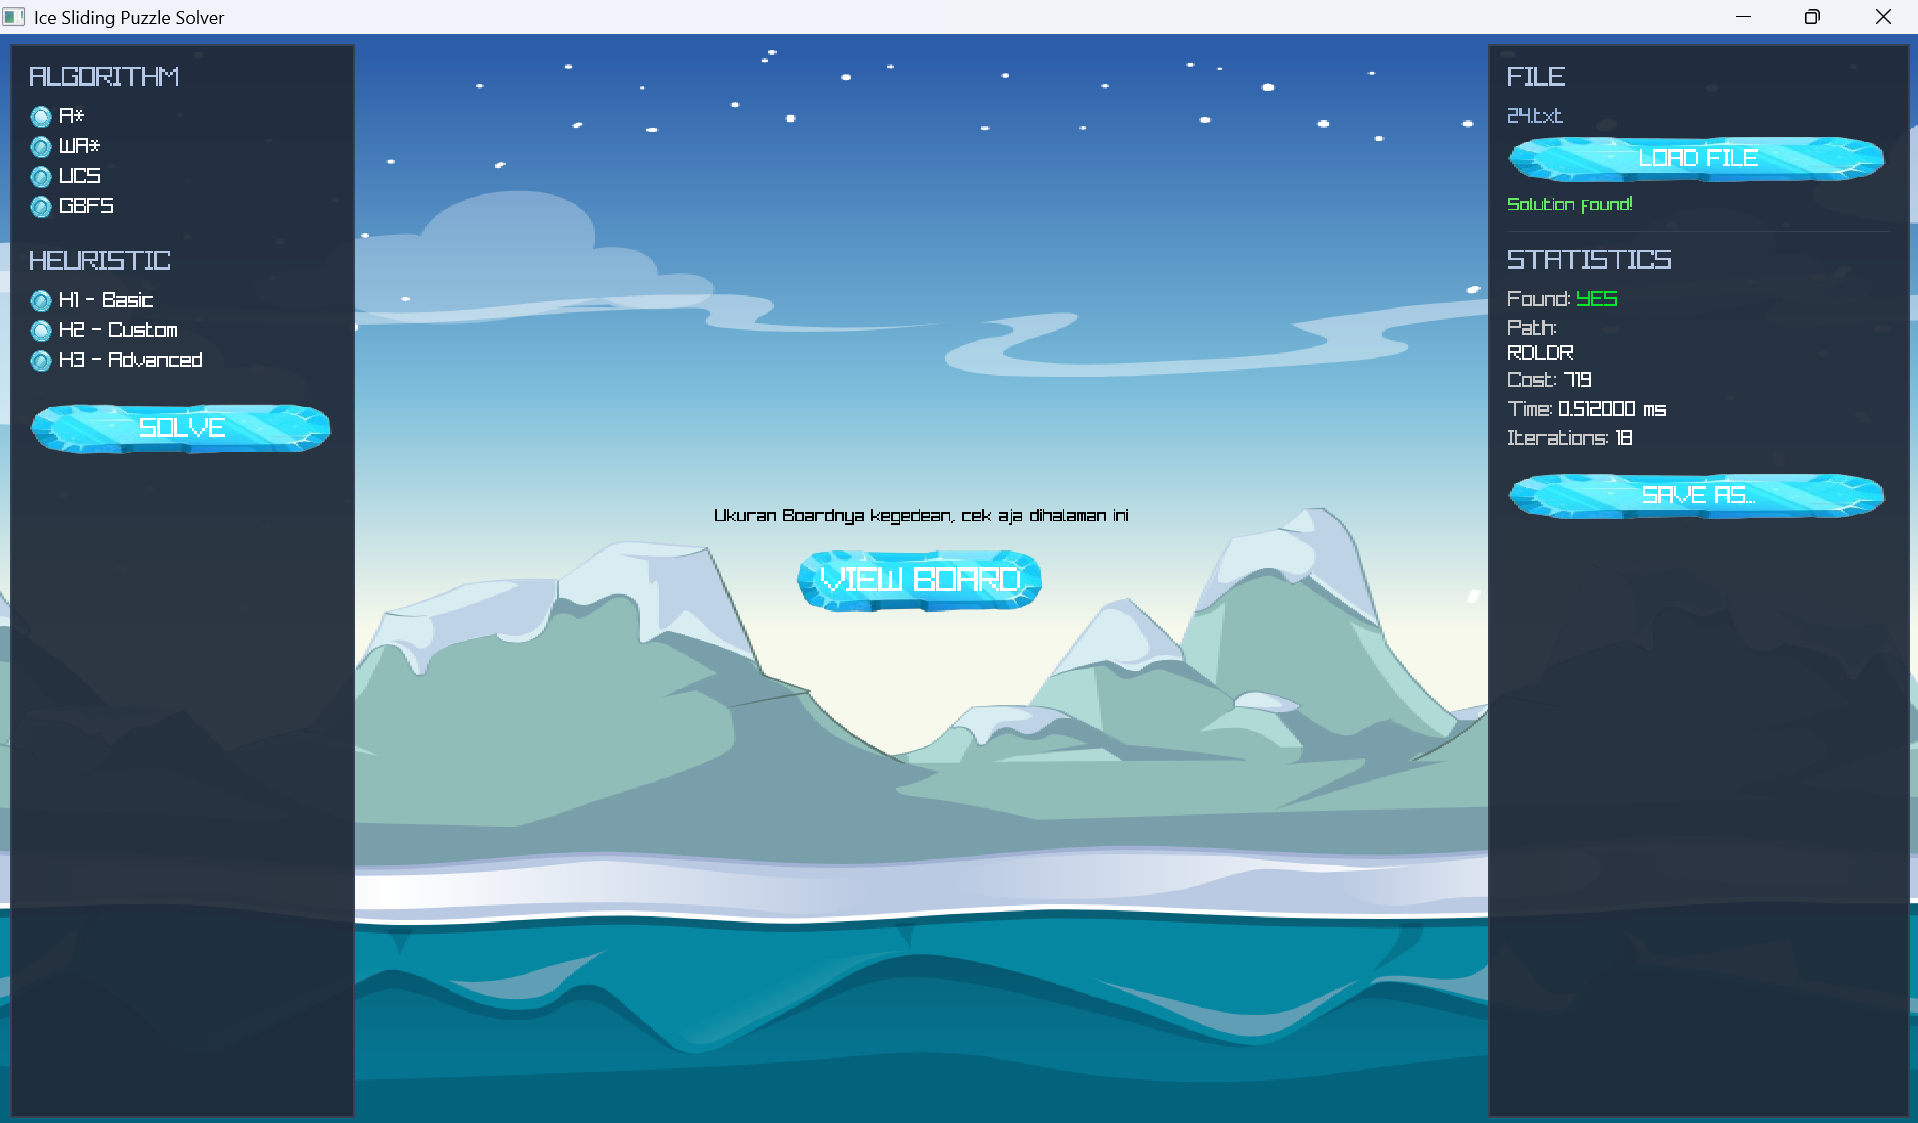
\includegraphics[width=\textwidth]{public/test24-A-h2.png}
		\caption{Output Test 24 menggunakan A* + H2}
	\end{minipage}
	\hfill
	\begin{minipage}{0.48\textwidth}
		\centering
		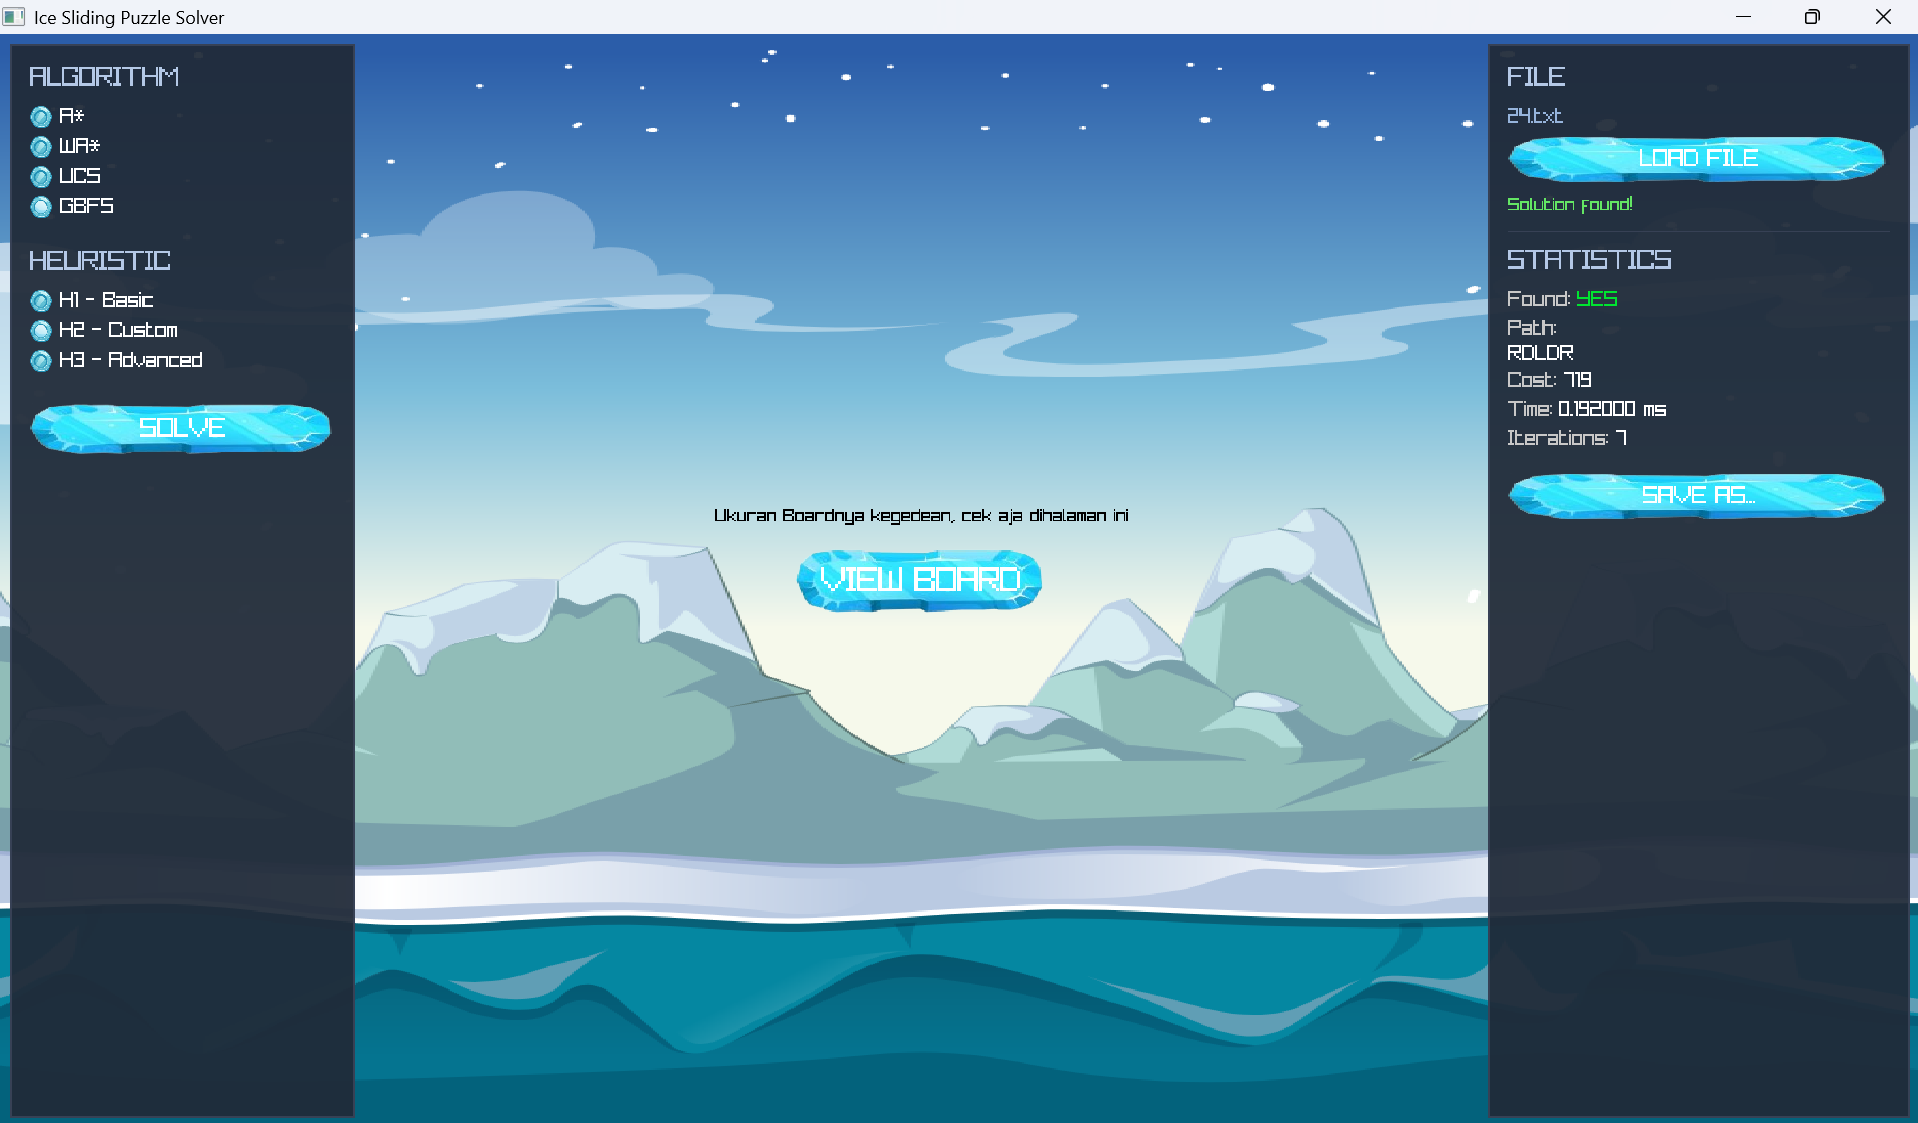
\includegraphics[width=\textwidth]{public/test24-GBFS-h2.png}
		\caption{Output Test 24 menggunakan GBFS + H2}
	\end{minipage}
\end{figure}

\begin{table}[H]
	\centering
	\caption{Hasil percobaan pada Test Case 24}
	\small
	\begin{tabular}{|p{4cm}|p{2.5cm}|p{2.5cm}|p{2.5cm}|}
		\hline
		\rowcolor{gray!20}
		\textbf{Algoritma} & \textbf{Cost} & \textbf{Time (ms)} & \textbf{Iterations} \\
		\hline
		A* - Basic & 719 & 0.229 & 17 \\
		\hline
		A* - Custom & 719 & 0.619 & 18 \\
		\hline
		A* - Advanced & 719 & 0.672 & 17 \\
		\hline
		WA* - Basic & 719 & 0.405 & 17 \\
		\hline
		WA* - Custom & 719 & 0.621 & 17 \\
		\hline
		WA* - Advanced & 719 & 0.534 & 17 \\
		\hline
		UCS & 719 & 0.339 & 17 \\
		\hline
		GBFS - Basic & 719 & 0.208 & 9 \\
		\hline
		GBFS - Custom & 719 & 0.192 & 7 \\
		\hline
		GBFS - Advanced & 719 & 0.356 & 7 \\
		\hline
	\end{tabular}
\end{table}

\begin{tcolorbox}[
	colback=green!5,
	colframe=green!50!black,
	title=\textbf{Ringkasan Test Case 24},
	arc=2mm,
	boxrule=0.8pt
]
Seluruh algoritma menghasilkan cost solusi yang sama, yaitu 719. 
GBFS dengan heuristik Custom dan Advanced memiliki jumlah iterasi paling kecil, yaitu 7 iterasi. 
Hal ini menunjukkan bahwa pada map ini, heuristik dapat membantu pencarian menemukan solusi valid dengan lebih cepat.
\end{tcolorbox}


\subsection{Test Case 25}

\begin{tcolorbox}[
	colback=blue!5,
	colframe=blue!60!black,
	title=\textbf{Ringkasan Input Test Case 25},
	arc=2mm,
	boxrule=0.8pt
]
Test case 25 menggunakan papan berukuran $12 \times 12$ dengan banyak obstacle dan lava. 
Tidak terdapat angka wajib, tetapi struktur map cukup kompleks karena banyak jalur yang dapat menjadi tidak valid apabila aktor melewati lava atau keluar dari lintasan aman.
\end{tcolorbox}

\begin{table}[H]
	\centering
	\caption{Karakteristik input Test Case 25}
	\begin{tabular}{|p{4cm}|p{9.5cm}|}
		\hline
		\rowcolor{blue!15}
		\textbf{Aspek} & \textbf{Keterangan} \\
		\hline
		Ukuran papan & $12 \times 12$ \\
		\hline
		Posisi awal & Ditandai dengan karakter \texttt{Z} pada kiri atas area map \\
		\hline
		Goal & Ditandai dengan karakter \texttt{O} di bagian tengah bawah map \\
		\hline
		Angka wajib & Tidak ada \\
		\hline
		Lava & Terdapat banyak tile \texttt{L} yang harus dihindari \\
		\hline
		Karakteristik utama & Map kompleks dengan banyak lava dan obstacle, sehingga cocok untuk menguji kemampuan algoritma mencari path valid yang aman. \\
		\hline
	\end{tabular}
\end{table}

\begin{tcolorbox}[
	colback=gray!5,
	colframe=black!60,
	title=\textbf{Isi File \texttt{25.txt}},
	arc=2mm,
	boxrule=0.8pt
]
\tiny
\begin{verbatim}
12 12
XXXXXXXXXXXX
XZ*********X
XXXXLXXLXX*X
XX*******X*X
XX*XXLXX*X*X
XX*X***X*X*X
XX*X*L*L*X*X
XX*L*X*X*X*X
XX*X**O**X*X
XX*XXLXXXX*X
XX*********X
XXXXXXXXXXXX
999 999 999 999 999 999 999 999 999 999 999 999
999 1 2 3 4 5 6 7 8 9 10 999
999 999 999 999 50 999 999 50 999 999 11 999
999 999 12 13 14 15 16 17 18 999 19 999
999 999 20 999 999 50 999 999 21 999 22 999
999 999 23 999 24 25 26 999 27 999 28 999
999 999 29 999 30 50 31 50 32 999 33 999
999 999 34 50 35 999 36 999 37 999 38 999
999 999 39 999 40 41 42 43 44 999 45 999
999 999 46 999 999 50 999 999 999 999 47 999
999 999 48 49 50 51 52 53 54 55 56 999
999 999 999 999 999 999 999 999 999 999 999 999
\end{verbatim}
\end{tcolorbox}

\begin{figure}[H]
	\centering
	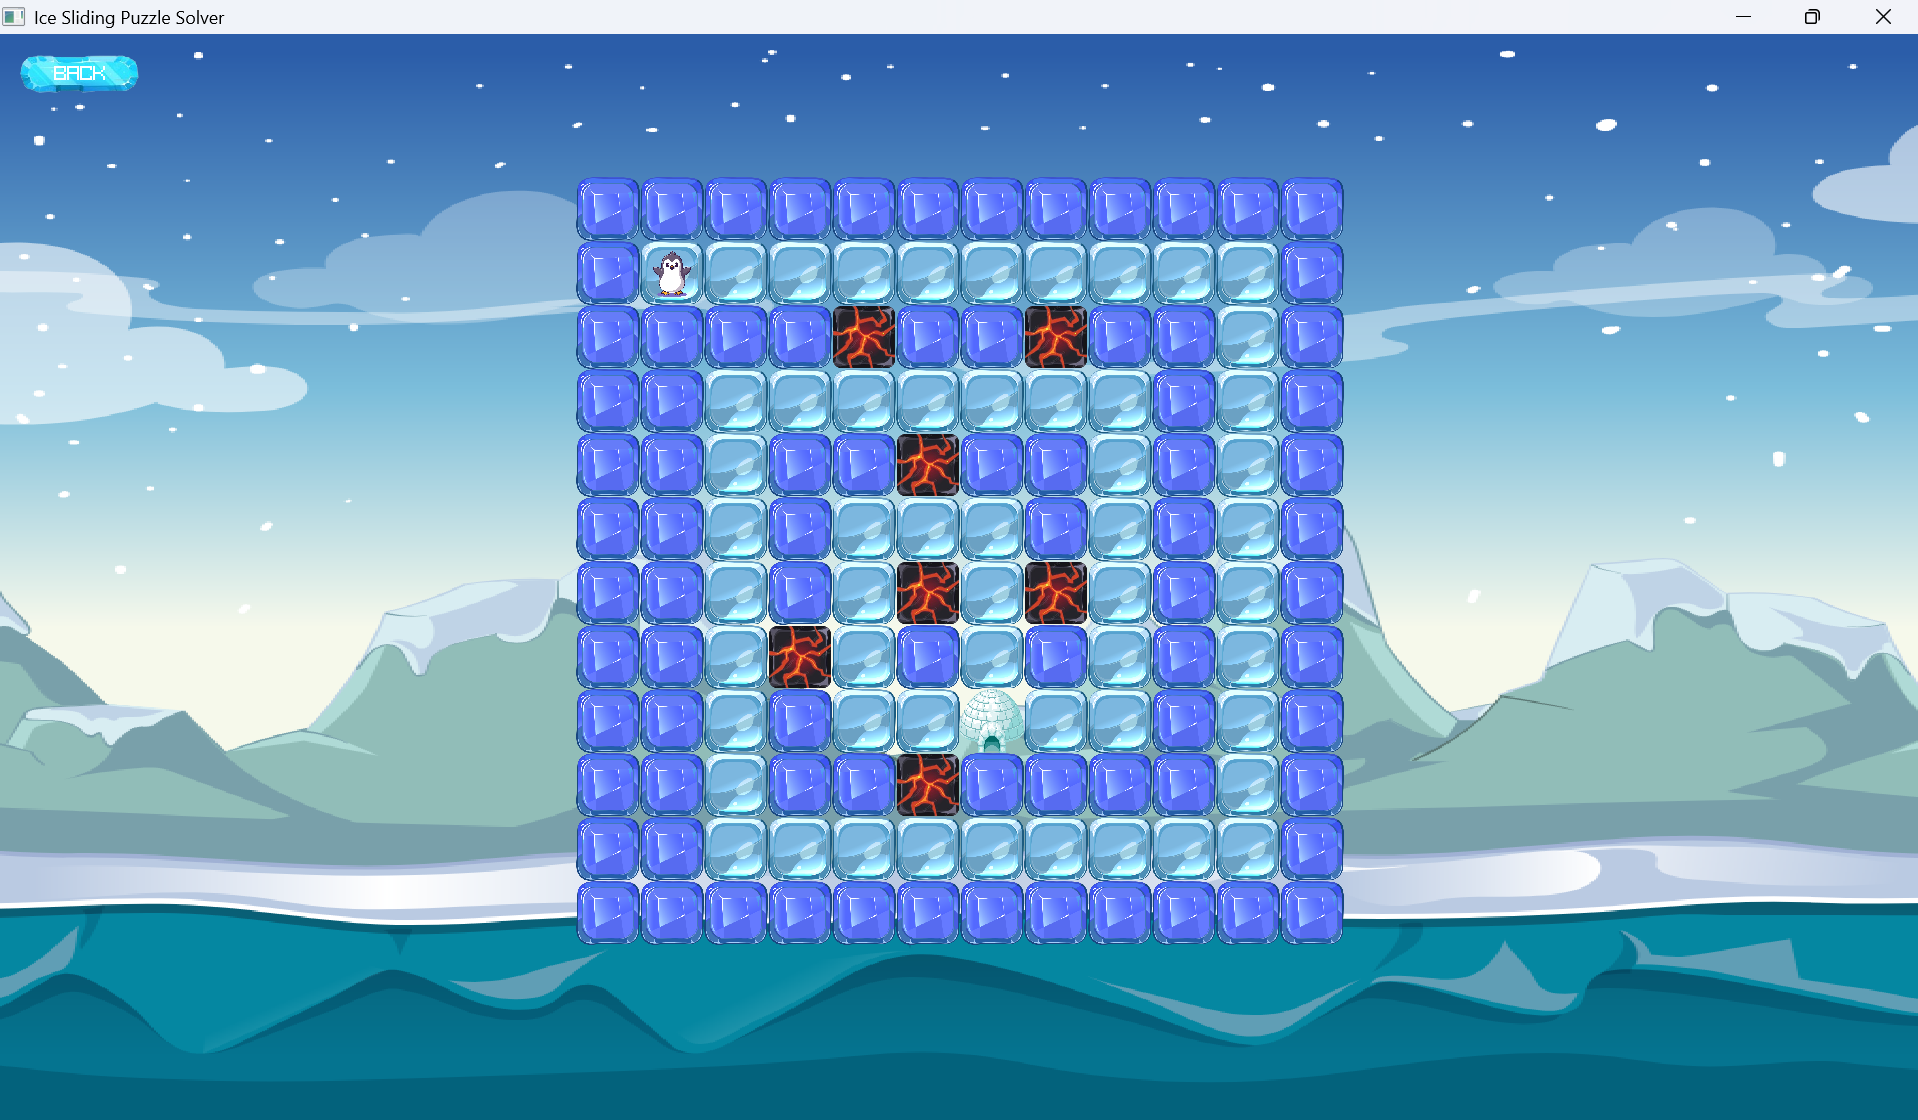
\includegraphics[width=0.65\textwidth]{public/map25.png}
	\caption{Visualisasi map pada Test Case 25}
\end{figure}

\begin{figure}[H]
	\centering
	\begin{minipage}{0.48\textwidth}
		\centering
		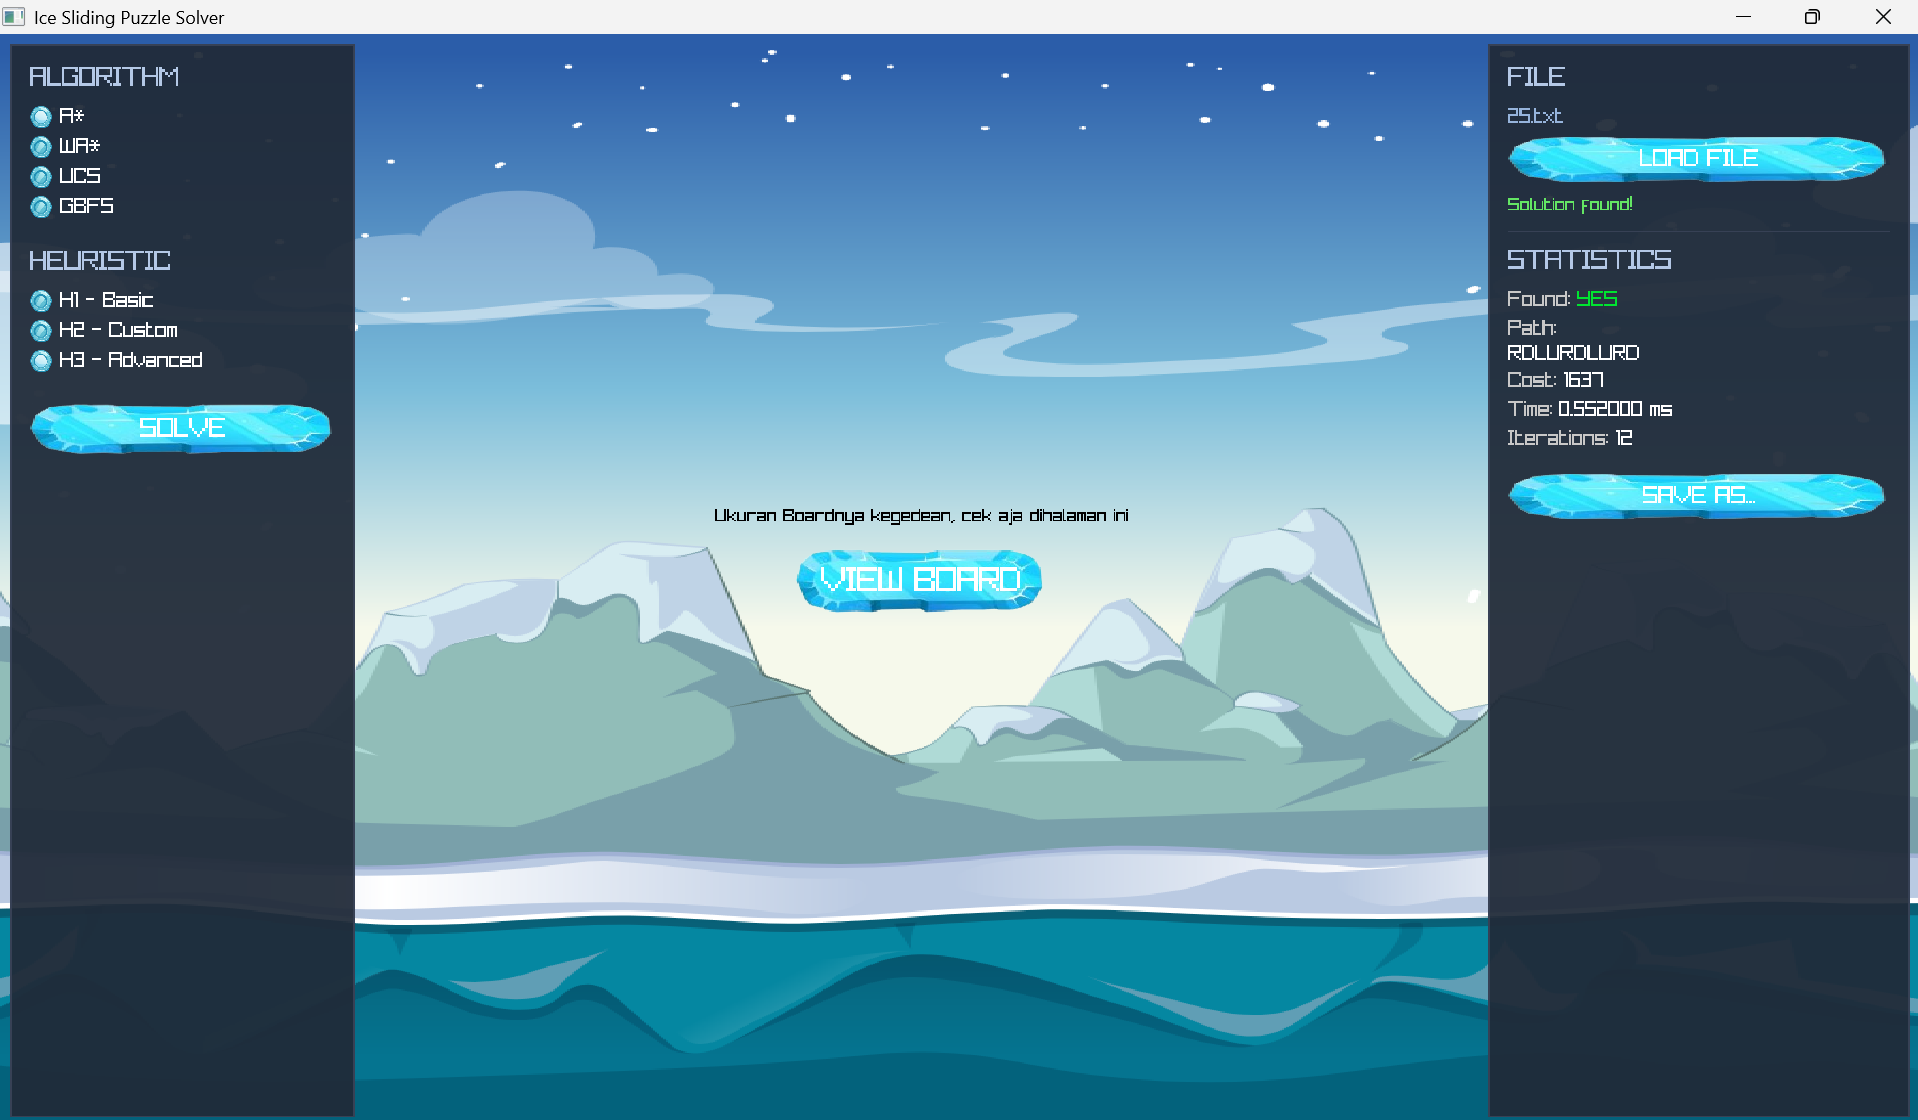
\includegraphics[width=\textwidth]{public/test25-A-h3.png}
		\caption{Output Test 25 menggunakan A* + H3}
	\end{minipage}
	\hfill
	\begin{minipage}{0.48\textwidth}
		\centering
		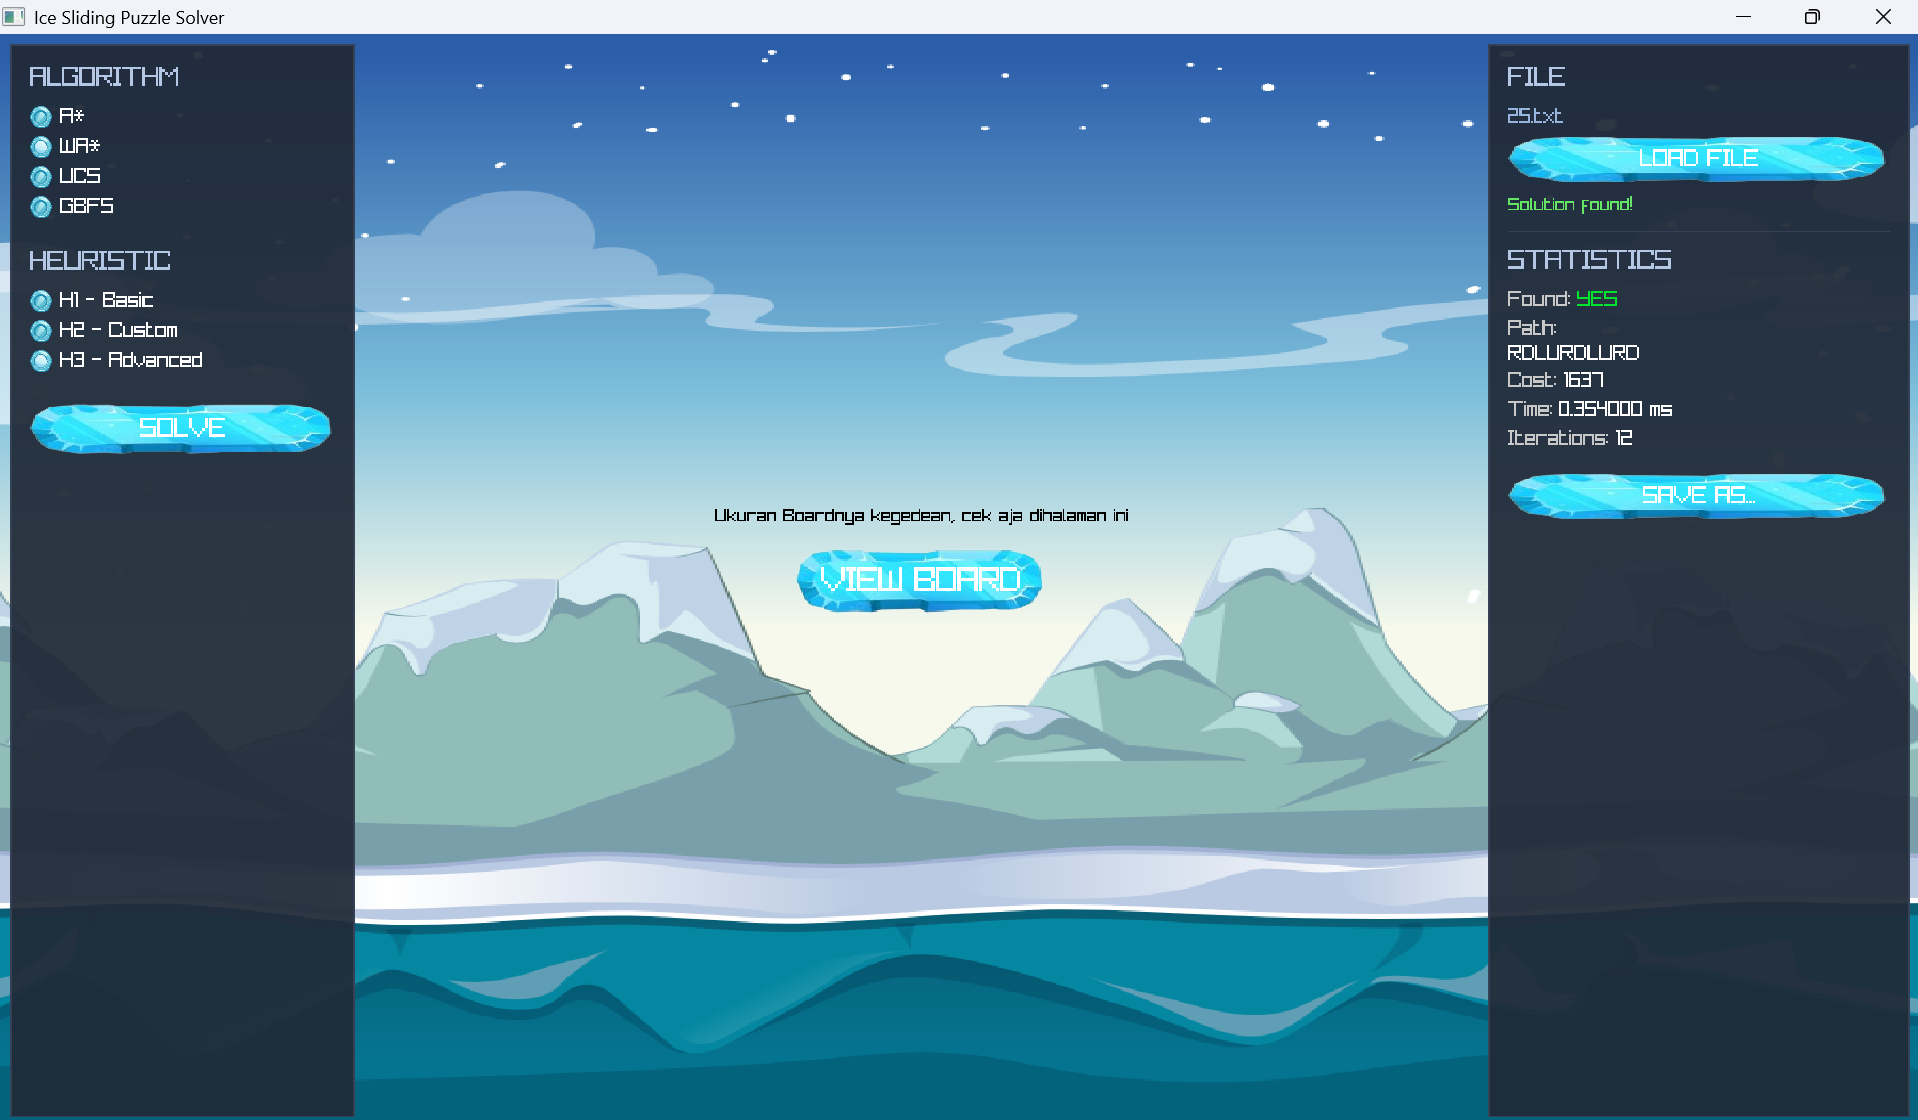
\includegraphics[width=\textwidth]{public/test25-WA-h3.png}
		\caption{Output Test 25 menggunakan Weighted A* + H3}
	\end{minipage}
\end{figure}

\begin{table}[H]
	\centering
	\caption{Hasil percobaan pada Test Case 25}
	\small
	\begin{tabular}{|p{4cm}|p{2.5cm}|p{2.5cm}|p{2.5cm}|}
		\hline
		\rowcolor{gray!20}
		\textbf{Algoritma} & \textbf{Cost} & \textbf{Time (ms)} & \textbf{Iterations} \\
		\hline
		A* - Basic & 1637 & 0.219 & 12 \\
		\hline
		A* - Custom & 1637 & 0.730 & 12 \\
		\hline
		A* - Advanced & 1637 & 0.949 & 12 \\
		\hline
		WA* - Basic & 1637 & 0.202 & 12 \\
		\hline
		WA* - Custom & 1637 & 0.296 & 12 \\
		\hline
		WA* - Advanced & 1637 & 0.354 & 12 \\
		\hline
		UCS & 1637 & 0.159 & 11 \\
		\hline
		GBFS - Basic & 1637 & 0.207 & 11 \\
		\hline
		GBFS - Custom & 1637 & 0.390 & 11 \\
		\hline
		GBFS - Advanced & 1637 & 0.388 & 11 \\
		\hline
	\end{tabular}
\end{table}

\begin{tcolorbox}[
	colback=green!5,
	colframe=green!50!black,
	title=\textbf{Ringkasan Test Case 25},
	arc=2mm,
	boxrule=0.8pt
]
Seluruh algoritma menghasilkan cost solusi yang sama, yaitu 1637. 
Meskipun map memiliki banyak lava dan obstacle, semua algoritma tetap dapat menemukan solusi valid. 
Perbedaan utama terlihat pada waktu eksekusi dan jumlah iterasi, bukan pada total cost solusi.
\end{tcolorbox}


\section{Ringkasan Hasil Tangkapan Layar}

Berdasarkan lima test case yang ditampilkan, program berhasil membaca input, menjalankan algoritma yang dipilih, dan menghasilkan output berupa solusi, cost, waktu eksekusi, serta jumlah iterasi. 
Setiap test case juga dilengkapi dengan visualisasi map dan dua tangkapan layar output sebagai bukti bahwa program dapat dijalankan pada beberapa konfigurasi papan yang berbeda.

\begin{table}[H]
	\centering
	\caption{Ringkasan pasangan tangkapan layar yang digunakan}
	\begin{tabular}{|p{2.2cm}|p{4.3cm}|p{4.3cm}|p{3cm}|}
		\hline
		\rowcolor{blue!15}
		\textbf{Test Case} & \textbf{Screenshot 1} & \textbf{Screenshot 2} & \textbf{Status} \\
		\hline
		Test 8 & GBFS + H3 & Weighted A* + H2 & Berhasil \\
		\hline
		Test 17 & GBFS + H1 & Weighted A* + H1 & Berhasil \\
		\hline
		Test 20 & A* + H1 & UCS & Berhasil \\
		\hline
		Test 24 & A* + H2 & GBFS + H2 & Berhasil \\
		\hline
		Test 25 & A* + H3 & Weighted A* + H3 & Berhasil \\
		\hline
	\end{tabular}
\end{table}
	
	\chapter{Analisa Eksperimen}
	Bagian ini membahas hasil percobaan algoritma pathfinding yang telah dilakukan pada lima test case, yaitu Test 8, Test 17, Test 20, Test 24, dan Test 25. 
Analisis dilakukan berdasarkan beberapa metrik utama, yaitu total cost solusi, waktu eksekusi, jumlah iterasi, stabilitas algoritma, dan pengaruh heuristik terhadap proses pencarian.

\begin{tcolorbox}[
	colback=blue!5,
	colframe=blue!60!black,
	title=\textbf{Tujuan Analisis Percobaan},
	arc=2mm,
	boxrule=0.8pt
]
Analisis ini bertujuan untuk membandingkan perilaku UCS, GBFS, A*, dan Weighted A* pada berbagai bentuk map. 
Setiap algoritma diuji untuk melihat kemampuan menemukan solusi, efisiensi jumlah iterasi, kecepatan eksekusi, serta kualitas cost solusi yang dihasilkan.
\end{tcolorbox}


\section{Deskripsi Umum Test Case}

Kelima test case yang digunakan memiliki karakteristik yang berbeda. 
Perbedaan tersebut meliputi ukuran papan, jumlah angka wajib, keberadaan lava, banyaknya rintangan, serta variasi cost tile. 
Perbedaan karakteristik ini penting karena dapat memengaruhi jumlah state yang dieksplorasi oleh setiap algoritma.

\begin{table}[H]
	\centering
	\caption{Deskripsi umum test case}
	\small
	\begin{tabular}{|p{2cm}|p{2cm}|p{2.2cm}|p{2cm}|p{4.8cm}|}
		\hline
		\rowcolor{blue!15}
		\textbf{Test Case} & \textbf{Ukuran} & \textbf{Angka Wajib} & \textbf{Lava} & \textbf{Karakteristik Map} \\
		\hline
		Test 8 & $6 \times 6$ & Tidak ada & Tidak ada & Map kecil dan sederhana untuk menguji mekanisme sliding dasar. \\
		\hline
		Test 17 & $10 \times 10$ & Ada, 0--7 & Tidak ada & Map besar dengan banyak angka dan variasi cost tile. \\
		\hline
		Test 20 & $12 \times 12$ & Tidak ada & Tidak ada & Map berbentuk maze dengan banyak rintangan. \\
		\hline
		Test 24 & $7 \times 12$ & Ada, 0--6 & Ada & Map dengan kombinasi angka berurutan, obstacle, dan lava. \\
		\hline
		Test 25 & $12 \times 12$ & Tidak ada & Ada & Map besar dengan banyak lava dan obstacle. \\
		\hline
	\end{tabular}
\end{table}

\begin{tcolorbox}[
	colback=gray!5,
	colframe=black!60,
	title=\textbf{Klasifikasi Tingkat Kesulitan Test Case},
	arc=2mm,
	boxrule=0.8pt
]
\begin{itemize}
	\item \textbf{Test 8} merupakan kasus sederhana karena ukuran kecil dan tidak memiliki angka maupun lava.
	\item \textbf{Test 17} menantang karena memiliki banyak angka yang harus dilewati secara berurutan.
	\item \textbf{Test 20} menantang dari sisi rintangan karena bentuknya menyerupai maze.
	\item \textbf{Test 24} menantang karena menggabungkan angka berurutan dan lava.
	\item \textbf{Test 25} menantang karena memiliki banyak lava dan obstacle, meskipun tidak memiliki angka wajib.
\end{itemize}
\end{tcolorbox}


\section{Metrik yang Dibandingkan}

Pada setiap percobaan, beberapa metrik digunakan untuk membandingkan performa algoritma. 
Metrik tersebut tidak hanya melihat apakah solusi ditemukan, tetapi juga memperhatikan efisiensi dan kualitas solusi.

\begin{table}[H]
	\centering
	\caption{Metrik pembanding hasil percobaan}
	\begin{tabular}{|p{4cm}|p{10cm}|}
		\hline
		\rowcolor{gray!20}
		\textbf{Metrik} & \textbf{Makna} \\
		\hline
		Total cost & Menunjukkan biaya total solusi yang ditemukan. Semakin kecil nilainya, semakin baik solusi dari sisi optimalitas cost. \\
		\hline
		Waktu eksekusi & Menunjukkan waktu yang dibutuhkan algoritma untuk menemukan solusi dalam milidetik. \\
		\hline
		Jumlah iterasi & Menunjukkan banyaknya state atau konfigurasi yang ditinjau selama pencarian. \\
		\hline
		Stabilitas & Menunjukkan kemampuan algoritma menghasilkan performa yang konsisten pada berbagai bentuk map. \\
		\hline
		Optimalitas & Menunjukkan apakah algoritma menghasilkan cost solusi minimum dibanding algoritma lain. \\
		\hline
		Efisiensi pencarian & Menunjukkan kemampuan algoritma menemukan solusi dengan jumlah iterasi dan waktu yang rendah. \\
		\hline
	\end{tabular}
\end{table}


\section{Rekapitulasi Hasil Percobaan}

Tabel berikut merangkum hasil terbaik dari setiap test case berdasarkan cost solusi, waktu eksekusi, dan jumlah iterasi.

\begin{longtable}{|p{2cm}|p{3.2cm}|p{3.2cm}|p{3.2cm}|}
	\caption{Rekapitulasi hasil terbaik per test case} \\
	\hline
	\rowcolor{green!15}
	\textbf{Test Case} & \textbf{Cost Terbaik} & \textbf{Waktu Tercepat} & \textbf{Iterasi Tersedikit} \\
	\hline
	\endfirsthead
	
	\hline
	\rowcolor{green!15}
	\textbf{Test Case} & \textbf{Cost Terbaik} & \textbf{Waktu Tercepat} & \textbf{Iterasi Tersedikit} \\
	\hline
	\endhead
	
	Test 8 & Semua algoritma, cost 37 & GBFS - Basic, 0.077 ms & GBFS, 3 iterasi \\
	\hline
	Test 17 & Semua algoritma, cost 1085 & GBFS - Custom, 0.439 ms & GBFS - Advanced, 10 iterasi \\
	\hline
	Test 20 & UCS, A*, WA*, cost 810 & GBFS - Basic, 0.065 ms & GBFS, 3 iterasi \\
	\hline
	Test 24 & Semua algoritma, cost 719 & GBFS - Custom, 0.192 ms & GBFS - Custom dan Advanced, 7 iterasi \\
	\hline
	Test 25 & Semua algoritma, cost 1637 & UCS, 0.159 ms & UCS dan GBFS, 11 iterasi \\
	\hline
\end{longtable}

\begin{tcolorbox}[
	colback=green!5,
	colframe=green!50!black,
	title=\textbf{Gambaran Umum Hasil},
	arc=2mm,
	boxrule=0.8pt
]
Sebagian besar test case menunjukkan bahwa semua algoritma dapat menemukan solusi valid. 
Perbedaan utama terlihat pada jumlah iterasi dan waktu eksekusi. 
Namun, pada Test 20, GBFS menghasilkan cost yang jauh lebih besar daripada UCS, A*, dan Weighted A*, sehingga terlihat bahwa GBFS tidak selalu aman untuk mencari solusi dengan cost minimum.
\end{tcolorbox}


\section{Analisis Per Test Case}

\subsection{Analisis Test Case 8}

Test Case 8 merupakan map kecil dan sederhana. 
Pada test case ini, semua algoritma menghasilkan cost solusi yang sama, yaitu 37. 
Hal ini menunjukkan bahwa pada map kecil tanpa angka dan lava, ruang pencarian relatif sederhana sehingga perbedaan strategi algoritma tidak terlalu memengaruhi kualitas cost solusi.

\begin{table}[H]
	\centering
	\caption{Analisis ringkas Test Case 8}
	\begin{tabular}{|p{4cm}|p{10cm}|}
		\hline
		\rowcolor{blue!15}
		\textbf{Aspek} & \textbf{Analisis} \\
		\hline
		Cost solusi & Semua algoritma menghasilkan cost 37. \\
		\hline
		Jumlah iterasi & GBFS membutuhkan 3 iterasi, lebih sedikit dibanding UCS yang membutuhkan 4 iterasi dan A*/WA* yang membutuhkan 5 iterasi. \\
		\hline
		Waktu eksekusi & Perbedaan waktu tidak terlalu signifikan karena ukuran map kecil. \\
		\hline
		Pengaruh heuristik & Tidak terlalu besar karena tidak ada angka dan struktur map sederhana. \\
		\hline
		Kesimpulan & Semua algoritma efektif pada map kecil, tetapi GBFS lebih efisien dari sisi iterasi. \\
		\hline
	\end{tabular}
\end{table}

\subsection{Analisis Test Case 17}

Test Case 17 memiliki banyak angka yang harus dilewati secara berurutan. 
Pada kasus ini, semua algoritma tetap menghasilkan cost solusi yang sama, yaitu 1085. 
Namun, jumlah iterasi berbeda cukup signifikan antara algoritma berbasis heuristik dan UCS/A*.

\begin{table}[H]
	\centering
	\caption{Analisis ringkas Test Case 17}
	\begin{tabular}{|p{4cm}|p{10cm}|}
		\hline
		\rowcolor{blue!15}
		\textbf{Aspek} & \textbf{Analisis} \\
		\hline
		Cost solusi & Semua algoritma menghasilkan cost 1085. \\
		\hline
		Constraint angka & Banyak angka menyebabkan state harus menyimpan progres angka melalui collected mask. \\
		\hline
		Jumlah iterasi & UCS dan A* berada di sekitar 71--72 iterasi, sedangkan GBFS dapat turun hingga 10--25 iterasi. \\
		\hline
		Pengaruh heuristik & Heuristik sangat membantu GBFS karena mampu mengarahkan pencarian menuju target angka berikutnya. \\
		\hline
		Kesimpulan & Pada map dengan banyak angka, heuristik yang sesuai dapat mengurangi jumlah iterasi secara signifikan. \\
		\hline
	\end{tabular}
\end{table}

\subsection{Analisis Test Case 20}

Test Case 20 merupakan map berbentuk maze dengan banyak rintangan. 
Pada test case ini, UCS, A*, dan Weighted A* menghasilkan cost 810, sedangkan GBFS menghasilkan cost 6174. 
Perbedaan ini menunjukkan risiko GBFS ketika heuristik terlalu berfokus pada kedekatan posisi tanpa mempertimbangkan cost aktual.

\begin{table}[H]
	\centering
	\caption{Analisis ringkas Test Case 20}
	\begin{tabular}{|p{4cm}|p{10cm}|}
		\hline
		\rowcolor{orange!20}
		\textbf{Aspek} & \textbf{Analisis} \\
		\hline
		Cost solusi & UCS, A*, dan WA* menghasilkan cost 810, sedangkan GBFS menghasilkan cost 6174. \\
		\hline
		Banyak rintangan & Rintangan membuat heuristik jarak menjadi kurang akurat karena jalur yang tampak dekat belum tentu murah. \\
		\hline
		Jumlah iterasi & GBFS hanya membutuhkan 3 iterasi, tetapi menghasilkan cost yang jauh lebih besar. \\
		\hline
		Optimalitas & UCS, A*, dan WA* lebih baik dari sisi cost pada test case ini. \\
		\hline
		Kesimpulan & GBFS cepat, tetapi pada map maze dapat memilih jalur yang tidak optimal dari sisi cost. \\
		\hline
	\end{tabular}
\end{table}

\subsection{Analisis Test Case 24}

Test Case 24 menggabungkan angka berurutan dan lava. 
Semua algoritma menghasilkan cost yang sama, yaitu 719. 
Meskipun terdapat lava, program tetap dapat menyaring jalur tidak valid melalui mekanisme \texttt{MovementEngine}.

\begin{table}[H]
	\centering
	\caption{Analisis ringkas Test Case 24}
	\begin{tabular}{|p{4cm}|p{10cm}|}
		\hline
		\rowcolor{blue!15}
		\textbf{Aspek} & \textbf{Analisis} \\
		\hline
		Cost solusi & Semua algoritma menghasilkan cost 719. \\
		\hline
		Lava & Gerakan yang melewati lava dianggap tidak valid sehingga tidak masuk ke state berikutnya. \\
		\hline
		Angka berurutan & Algoritma harus tetap mengikuti urutan angka sebelum menuju goal. \\
		\hline
		Jumlah iterasi & GBFS dengan Custom dan Advanced hanya membutuhkan 7 iterasi, lebih sedikit dibanding UCS, A*, dan WA*. \\
		\hline
		Kesimpulan & Heuristik efektif pada map ini karena mampu mengarahkan pencarian meskipun terdapat lava dan angka wajib. \\
		\hline
	\end{tabular}
\end{table}

\subsection{Analisis Test Case 25}

Test Case 25 memiliki banyak lava dan obstacle, tetapi tidak memiliki angka wajib. 
Semua algoritma menghasilkan cost yang sama, yaitu 1637. 
Hal ini menunjukkan bahwa meskipun map cukup kompleks, jalur solusi yang valid relatif terarah sehingga semua algoritma dapat menemukan solusi dengan cost yang sama.

\begin{table}[H]
	\centering
	\caption{Analisis ringkas Test Case 25}
	\begin{tabular}{|p{4cm}|p{10cm}|}
		\hline
		\rowcolor{blue!15}
		\textbf{Aspek} & \textbf{Analisis} \\
		\hline
		Cost solusi & Semua algoritma menghasilkan cost 1637. \\
		\hline
		Lava dan obstacle & Banyak jalur berisiko menyebabkan game over, sehingga validasi gerakan sangat penting. \\
		\hline
		Jumlah iterasi & UCS dan GBFS membutuhkan 11 iterasi, sedangkan A* dan WA* membutuhkan 12 iterasi. \\
		\hline
		Waktu eksekusi & UCS menjadi yang tercepat pada hasil percobaan ini. \\
		\hline
		Kesimpulan & Pada map ini, semua algoritma stabil dan menghasilkan kualitas solusi yang sama. \\
		\hline
	\end{tabular}
\end{table}


\section{Analisis Per Algoritma}

\subsection{Uniform Cost Search}

UCS selalu memilih state berdasarkan cost aktual terkecil. 
Berdasarkan hasil percobaan, UCS konsisten menghasilkan cost solusi terbaik atau sama dengan algoritma terbaik lainnya pada seluruh test case.

\begin{table}[H]
	\centering
	\caption{Analisis performa UCS}
	\begin{tabular}{|p{4cm}|p{10cm}|}
		\hline
		\rowcolor{green!15}
		\textbf{Aspek} & \textbf{Analisis} \\
		\hline
		Optimalitas & UCS paling aman untuk mencari total cost minimum karena selalu memperluas state dengan cost aktual terkecil. \\
		\hline
		Map kecil & Pada Test 8, UCS menghasilkan cost optimal dengan iterasi sedikit. \\
		\hline
		Map besar & Pada Test 17, UCS membutuhkan lebih banyak iterasi dibanding GBFS, tetapi tetap menghasilkan cost terbaik. \\
		\hline
		Map banyak tembok & Pada Test 20, UCS menghasilkan cost 810, jauh lebih baik daripada GBFS yang menghasilkan cost 6174. \\
		\hline
		Kelebihan & Sangat cocok untuk map dengan cost tile bervariasi. \\
		\hline
		Kekurangan & Tidak menggunakan informasi arah tujuan, sehingga pada beberapa kasus jumlah iterasi lebih besar. \\
		\hline
	\end{tabular}
\end{table}

\subsection{Greedy Best-First Search}

GBFS memilih state berdasarkan nilai heuristik terkecil. 
Hasil percobaan menunjukkan bahwa GBFS sering memiliki jumlah iterasi paling sedikit, tetapi tidak selalu menghasilkan cost terbaik.

\begin{table}[H]
	\centering
	\caption{Analisis performa GBFS}
	\begin{tabular}{|p{4cm}|p{10cm}|}
		\hline
		\rowcolor{orange!20}
		\textbf{Aspek} & \textbf{Analisis} \\
		\hline
		Kecepatan & GBFS sering menjadi algoritma dengan waktu eksekusi paling cepat. \\
		\hline
		Jumlah iterasi & Pada Test 8, Test 17, Test 20, dan Test 24, GBFS memiliki iterasi lebih sedikit dibanding algoritma lain. \\
		\hline
		Risiko optimalitas & Pada Test 20, GBFS menghasilkan cost 6174, jauh lebih besar daripada cost terbaik 810. \\
		\hline
		Pengaruh heuristik & Performa GBFS sangat bergantung pada kualitas heuristik yang digunakan. \\
		\hline
		Kelebihan & Sangat efisien untuk menemukan solusi dengan cepat. \\
		\hline
		Kekurangan & Tidak aman digunakan jika tujuan utama adalah cost minimum. \\
		\hline
	\end{tabular}
\end{table}

\subsection{A*}

A* menggabungkan cost aktual dan heuristik melalui fungsi $f(n)=g(n)+h(n)$. 
Berdasarkan hasil percobaan, A* menghasilkan cost terbaik pada seluruh test case, termasuk pada Test 20 yang menunjukkan kelemahan GBFS.

\begin{table}[H]
	\centering
	\caption{Analisis performa A*}
	\begin{tabular}{|p{4cm}|p{10cm}|}
		\hline
		\rowcolor{red!15}
		\textbf{Aspek} & \textbf{Analisis} \\
		\hline
		Keseimbangan & A* menyeimbangkan cost aktual dan estimasi menuju target. \\
		\hline
		Kualitas solusi & A* menghasilkan cost yang sama dengan UCS pada seluruh test case. \\
		\hline
		Jumlah iterasi & A* dapat memiliki iterasi lebih besar dari GBFS, tetapi lebih aman dari sisi cost. \\
		\hline
		Map banyak tembok & Pada Test 20, A* tetap menghasilkan cost 810, sedangkan GBFS menghasilkan cost 6174. \\
		\hline
		Stabilitas & A* stabil pada berbagai bentuk map karena tetap mempertimbangkan cost aktual. \\
		\hline
		Kesimpulan & A* merupakan algoritma paling seimbang antara optimalitas dan efisiensi pencarian. \\
		\hline
	\end{tabular}
\end{table}

\subsection{Weighted A*}

Weighted A* menggunakan fungsi evaluasi $f(n)=g(n)+2h(n)$, sehingga heuristik memiliki pengaruh lebih besar daripada A* biasa. 
Tujuannya adalah mempercepat pencarian dengan membuat algoritma lebih agresif menuju target.

\begin{table}[H]
	\centering
	\caption{Analisis performa Weighted A*}
	\begin{tabular}{|p{4cm}|p{10cm}|}
		\hline
		\rowcolor{purple!15}
		\textbf{Aspek} & \textbf{Analisis} \\
		\hline
		Pengaruh bobot & Bobot $w=2$ membuat algoritma lebih mengikuti heuristik dibanding A* biasa. \\
		\hline
		Kualitas solusi & Pada percobaan ini, Weighted A* menghasilkan cost yang sama dengan A* pada seluruh test case. \\
		\hline
		Jumlah iterasi & Jumlah iterasi Weighted A* umumnya sama dengan A* pada data uji yang digunakan. \\
		\hline
		Waktu eksekusi & Pada beberapa kasus, Weighted A* lebih cepat daripada A*, misalnya Test 20 dan Test 25. \\
		\hline
		Risiko & Secara teori, Weighted A* tidak selalu menjamin solusi optimal karena heuristik diperbesar. \\
		\hline
		Kesimpulan & Weighted A* cocok sebagai algoritma bonus untuk menguji trade-off antara kecepatan dan optimalitas. \\
		\hline
	\end{tabular}
\end{table}


\section{Analisis Pengaruh Heuristik}

Heuristik yang digunakan pada percobaan adalah H1, H2, dan H3. 
Berdasarkan implementasi program, H1 merepresentasikan Manhattan menuju goal, H2 mengarah ke angka berikutnya atau goal, sedangkan H3 memperkirakan beberapa target yang belum dikumpulkan.

\begin{longtable}{|p{2cm}|p{4cm}|p{7.5cm}|}
	\caption{Karakteristik heuristik} \\
	\hline
	\rowcolor{orange!20}
	\textbf{Heuristik} & \textbf{Nama} & \textbf{Karakteristik} \\
	\hline
	\endfirsthead
	
	\hline
	\rowcolor{orange!20}
	\textbf{Heuristik} & \textbf{Nama} & \textbf{Karakteristik} \\
	\hline
	\endhead
	
	H1 & Basic / Manhattan & Menghitung jarak Manhattan langsung menuju goal. Cepat dihitung, tetapi tidak memperhatikan angka berikutnya. \\
	\hline
	H2 & Custom & Menghitung jarak ke angka berikutnya yang harus dikumpulkan, lalu menuju goal jika semua angka selesai. \\
	\hline
	H3 & Advanced & Mengestimasi sisa perjalanan ke target-target yang belum dikumpulkan dan goal dengan pendekatan greedy. \\
	\hline
\end{longtable}

\begin{table}[H]
	\centering
	\caption{Analisis pengaruh heuristik terhadap algoritma}
	\begin{tabular}{|p{4cm}|p{10cm}|}
		\hline
		\rowcolor{orange!20}
		\textbf{Aspek} & \textbf{Analisis} \\
		\hline
		Pengaruh pada GBFS & Sangat besar, karena GBFS hanya menggunakan $h(n)$ sebagai prioritas. Pada Test 17 dan Test 24, heuristik Custom dan Advanced menurunkan jumlah iterasi secara signifikan. \\
		\hline
		Pengaruh pada A* & Cukup besar, tetapi tidak sedominan GBFS karena A* tetap mempertimbangkan $g(n)$. \\
		\hline
		Pengaruh pada Weighted A* & Lebih besar dibanding A* karena nilai heuristik dikalikan bobot $2$. \\
		\hline
		Heuristik paling cepat & Pada beberapa test case, Custom menghasilkan waktu terbaik, misalnya Test 17 dan Test 24 pada GBFS. \\
		\hline
		Heuristik paling stabil & Custom cukup stabil untuk map dengan angka karena targetnya mengikuti angka berikutnya. \\
		\hline
		Risiko heuristik & Heuristik yang tidak memperhitungkan obstacle, lava, dan sliding dapat mengarahkan algoritma ke jalur yang tampak dekat tetapi tidak optimal. \\
		\hline
	\end{tabular}
\end{table}


\section{Perbandingan Teoritis dan Eksperimental}

Secara teori, UCS menjamin cost minimum untuk cost positif, GBFS cepat tetapi tidak optimal, A* menyeimbangkan cost dan heuristik, sedangkan Weighted A* memperbesar pengaruh heuristik untuk mempercepat pencarian. 
Hasil percobaan secara umum sesuai dengan teori tersebut.

\begin{table}[H]
	\centering
	\caption{Perbandingan teori dan hasil eksperimen}
	\begin{tabular}{|p{3cm}|p{5cm}|p{6cm}|}
		\hline
		\rowcolor{gray!20}
		\textbf{Algoritma} & \textbf{Ekspektasi Teoritis} & \textbf{Hasil Eksperimen} \\
		\hline
		UCS & Optimal tetapi dapat mengeksplorasi banyak state. & Menghasilkan cost terbaik pada semua test case, tetapi tidak selalu memiliki iterasi paling kecil. \\
		\hline
		GBFS & Cepat, tetapi tidak selalu optimal. & Sering memiliki iterasi paling kecil, tetapi pada Test 20 menghasilkan cost jauh lebih besar. \\
		\hline
		A* & Seimbang antara cost aktual dan heuristik. & Menghasilkan cost terbaik dan lebih stabil daripada GBFS. \\
		\hline
		Weighted A* & Lebih agresif mengikuti heuristik dan dapat lebih cepat, tetapi tidak selalu optimal. & Pada percobaan ini cost tetap sama dengan A*, tetapi secara teori masih memiliki risiko menghasilkan cost lebih besar. \\
		\hline
	\end{tabular}
\end{table}

\begin{tcolorbox}[
	colback=gray!5,
	colframe=black!60,
	title=\textbf{Faktor Penyebab Perbedaan Hasil},
	arc=2mm,
	boxrule=0.8pt
]
Perbedaan hasil antar algoritma dipengaruhi oleh beberapa faktor, yaitu bentuk map, jumlah tembok, keberadaan angka, variasi cost tile, kualitas heuristik, banyaknya gerakan yang menyebabkan game over, dan ukuran papan. 
Pada map dengan banyak rintangan, heuristik jarak dapat menjadi kurang akurat karena jalur yang tampak dekat belum tentu dapat dicapai dengan cost rendah.
\end{tcolorbox}


\section{Kesimpulan Hasil Percobaan}

Berdasarkan seluruh hasil percobaan, dapat disimpulkan bahwa setiap algoritma memiliki keunggulan dan kelemahan masing-masing.

\begin{table}[H]
	\centering
	\caption{Kesimpulan hasil percobaan}
	\begin{tabular}{|p{5cm}|p{9cm}|}
		\hline
		\rowcolor{green!15}
		\textbf{Kategori} & \textbf{Kesimpulan} \\
		\hline
		Algoritma terbaik dari sisi optimalitas & UCS dan A* karena selalu menghasilkan cost terbaik pada seluruh test case. \\
		\hline
		Algoritma terbaik dari sisi waktu & GBFS sering menjadi yang tercepat, terutama pada Test 8, Test 17, Test 20, dan Test 24. \\
		\hline
		Algoritma terbaik dari sisi iterasi & GBFS karena sering meninjau state paling sedikit. \\
		\hline
		Algoritma terbaik untuk map kecil & GBFS cukup unggul karena dapat menemukan solusi dengan iterasi sedikit. \\
		\hline
		Algoritma terbaik untuk map banyak angka & GBFS dengan heuristik Custom atau Advanced efektif mengurangi iterasi, tetapi A* lebih aman untuk menjaga kualitas cost. \\
		\hline
		Algoritma terbaik untuk map banyak tembok & UCS dan A* lebih aman karena mempertimbangkan cost aktual. \\
		\hline
		Heuristik terbaik secara umum & Custom cukup baik karena mempertimbangkan angka berikutnya, sehingga lebih sesuai dengan constraint puzzle. \\
		\hline
		Rekomendasi algoritma utama & A* direkomendasikan sebagai algoritma utama karena memberikan keseimbangan antara kualitas cost solusi dan efisiensi pencarian. \\
		\hline
	\end{tabular}
\end{table}

\begin{tcolorbox}[
	colback=green!5,
	colframe=green!50!black,
	title=\textbf{Kesimpulan Akhir},
	arc=2mm,
	boxrule=0.8pt
]
UCS paling aman untuk memperoleh solusi dengan cost minimum, tetapi dapat membutuhkan eksplorasi lebih besar. 
GBFS paling cepat dari sisi iterasi dan waktu, tetapi berisiko menghasilkan solusi mahal seperti pada Test 20. 
A* menjadi pilihan paling seimbang karena tetap mempertimbangkan cost aktual dan heuristik. 
Weighted A* berguna sebagai algoritma bonus untuk mengevaluasi trade-off antara kecepatan dan optimalitas, terutama ketika heuristik ingin diberi pengaruh lebih besar.
\end{tcolorbox}

	\chapter{Lampiran}
	\section{Pranala Repository}

Source code program dapat diakses melalui pranala repository berikut:

\begin{tcolorbox}[
	colback=blue!5,
	colframe=blue!60!black,
	title=\textbf{Repository Program},
	arc=2mm,
	boxrule=0.8pt
]
\noindent
\textbf{Nama Repository:} \texttt{Tucil3\_NIM1\_NIM2}

\vspace{0.2cm}

\noindent
\textbf{Pranala Repository:}

\begin{center}
	\texttt{https://github.com/agathatatiana936/Tucil3\_13524008\_13524028}
\end{center}
\end{tcolorbox}

\section{Checklist Spesifikasi Program}

\begin{table}[H]
	\centering
	\caption{Checklist pemenuhan spesifikasi program}
	\renewcommand{\arraystretch}{1.4}
	\begin{tabular}{|c|p{9cm}|c|c|}
		\hline
		\rowcolor{gray!20}
		\textbf{No} & \centering\arraybackslash\textbf{Poin} & \textbf{Ya} & \textbf{Tidak} \\
		\hline
		1 & Program berhasil dikompilasi tanpa kesalahan & \checkmark & \\
		\hline
		2 & Program berhasil dijalankan & \checkmark & \\
		\hline
		3 & Solusi yang diberikan program benar dan mematuhi aturan permainan & \checkmark & \\
		\hline
		4 & Program dapat membaca masukan berkas \texttt{.txt} serta menyimpan solusi dalam berkas \texttt{.txt} & \checkmark & \\
		\hline
		5 & Program memiliki \textit{Graphical User Interface} (GUI) & \checkmark & \\
		\hline
		6 & Ada algoritma \textit{pathfinding} alternatif selain dari spesifikasi wajib, yaitu Weighted A* & \checkmark & \\
		\hline
		7 & Ada tambahan dua alternatif heuristik selain yang utama, yaitu Custom dan Advanced & \checkmark & \\
		\hline
	\end{tabular}
\end{table}


\section{Pernyataan Tidak Melakukan Kecurangan}

\begin{tcolorbox}[
	colback=white,
	colframe=black,
	arc=0mm,
	boxrule=0.8pt,
	left=3mm,
	right=3mm,
	top=3mm,
	bottom=3mm
]
Tugas ini disusun sepenuhnya tanpa bantuan kecerdasan buatan (\textit{Generative AI}), melainkan hasil pemikiran dan analisis mandiri.

\vspace{1.2cm}

\begin{center} 
\begin{tabular}{p{6cm}p{6cm}}
	\centering
	
\includegraphics[height=1.8cm]{public/ttd-anggota1.png}
	&
	\centering
	
\includegraphics[height=1.8cm]{public/ttd-anggota2.png}
	\tabularnewline[-0.1cm]
	
	\centering
	\rule{5cm}{0.4pt}
	&
	\centering
	\rule{5cm}{0.4pt}
	\tabularnewline
	
	\centering
	\textbf{Agatha Tatianingseto}
	&
	\centering
	\textbf{Muhammad Nur Majiid}
	\tabularnewline
	
	\centering
	13524008
	&
	\centering
	13524028
	\tabularnewline
\end{tabular}
\end{center}
\end{tcolorbox}
	
	\bibliography{dafpus}
	
\end{document}
